%%%%%%%%%%%%%%%%%%%%%%%%%%%%%%%%%%%%%%%%%%%%%%%%%%%%%%%%%%%%%%%%%%%%%%%%%%%%%%%
%%
%%          $Id: Rulebook.tex 2014-12-12 balkce $
%%    author(s): RoboCupAtHome Technical Committee(s)
%%  description: introduction to RoboCupAtHome
%%
%%%%%%%%%%%%%%%%%%%%%%%%%%%%%%%%%%%%%%%%%%%%%%%%%%%%%%%%%%%%%%%%%%%%%%%%%%%%%%%
\documentclass[11pt, twoside, openright, a4paper, chapterprefix]{scrbook}
\usepackage[inner=2.5cm, outer=2.5cm, top=4cm, bottom=4cm]{geometry}

%%% PACKAGES %%%%%%%%%%%%%%%%%%%%%%%%%%%%%%%%%%%%%%%%%%%%%%%%%%%%%%%%%%%%%%%%%%
%%%%%%%%%%%%%%%%%%%%%%%%%%%%%%%%%%%%%%%%%%%%%%%%%%%%%%%%%%%%%%%%%%%%%%%%%%%%%%%
%%
%%          $Id: packages.tex 385 2013-02-12 21:53:10Z holz $
%%    author(s): RoboCupAtHome Technical Committee(s)
%%  description: List of packages for the RoboCupAtHome rulebook
%%
%%%%%%%%%%%%%%%%%%%%%%%%%%%%%%%%%%%%%%%%%%%%%%%%%%%%%%%%%%%%%%%%%%%%%%%%%%%%%%%
% \usepackage{soul}

\usepackage[utf8x]{inputenc}
\usepackage[english]{babel}
\usepackage{amsmath,amssymb,amsfonts}
% \usepackage[nice]{nicefrac}
\usepackage{siunitx}
\usepackage{graphicx}
\usepackage{multicol}
\usepackage{verbatim}
\usepackage{fancyhdr}

% \usepackage{color}
\usepackage{xcolor}
\usepackage{colortbl}
% \usepackage{epsfig}
\usepackage{makeidx} % This one causes scoresheets not to setle
% \usepackage{lscape}
% \usepackage{picinpar}

\usepackage{./styles/tweaklist}

\usepackage{enumerate}
\usepackage{paralist}
\usepackage{multirow}
\usepackage{pgffor}
% \usepackage{array}

\usepackage{hyperref}
\usepackage{tabularx}
\usepackage{xspace}
\usepackage{csquotes}
\usepackage[inline]{enumitem}

%\usepackage{times}
%\usepackage{helvet}
%\usepackage{courier}

% \usepackage{url}
\usepackage{caption}
% \usepackage{epstopdf}
\usepackage{subfig}
\usepackage{float}
\usepackage{wrapfig}
% \usepackage{xfrac}

% \usepackage[titletoc]{appendix}
% \usepackage{enumitem}
% \usepackage{mathtools}
% \usepackage{gensymb}

% Required by scoresheets
\usepackage{calc}
\usepackage{ifthen}
\usepackage{environ}
\usepackage{wasysym}
\usepackage{chngpage}

% Local Variables:
% TeX-master: "../Rulebook"
% End:

\usepackage[titletoc]{appendix}
\usepackage{enumitem}
\usepackage{mathtools}
\usepackage{gensymb}
\setlist{noitemsep}

%%% SubfigureSetup %%%%%%%%%%%%%%%%%%%%%%%%%%%%%%%%%%%%%%%%%%%%%%%%%%%%%%%%%%%%
%\renewcommand{\subfigtopskip}{5pt}        % default is 10pt
%\renewcommand{\subfigbottomskip}{5pt}     % default is 10pt
%\renewcommand{\subfigcapskip}{3pt}        % default is 10pt
%\renewcommand{\subfigcapmargin}{7pt}      % default is 10pt

%%% TweakList-Setup %%%%%%%%%%%%%%%%%%%%%%%%%%%%%%%%%%%%%%%%%%%%%%%%%%%%%%%%%%%
\renewcommand{\itemhook}{%                 % modify itemize-spacing
  \setlength{\topsep}{2pt}%
  \setlength{\partopsep}{1pt}%
  \setlength{\itemsep}{-1pt}%
}
\renewcommand{\enumhook}{%                 % modify enumerate-spacing
  \setlength{\topsep}{2pt}%
  \setlength{\partopsep}{1pt}%
  \setlength{\itemsep}{-1pt}%
}
\renewcommand{\descripthook}{%             % modify description-spacing
  \setlength{\topsep}{2pt}%
  \setlength{\partopsep}{1pt}%
  \setlength{\itemsep}{-1pt}%
}

\setkomafont{title}{\normalfont}
\setkomafont{sectioning}{\normalfont\bfseries}
\addtokomafont{caption}{\small}
\setkomafont{captionlabel}{\small\bfseries}
\setkomafont{descriptionlabel}{\normalfont\bfseries}
\renewcommand*{\chapterformat}{\LARGE{Chapter \thechapter}}

%%% MACROS %%%%%%%%%%%%%%%%%%%%%%%%%%%%%%%%%%%%%%%%%%%%%%%%%%%%%%%%%%%%%%%%%%%%
\newcommand{\YEAR}{2017}
% \newcommand{\STATE}{Draft}
 \newcommand{\STATE}{Final}

% Local Variables:
% TeX-master: "../Rulebook"
% End:

\graphicspath{{\YEAR/}{./images/}}
%%%%%%%%%%%%%%%%%%%%%%%%%%%%%%%%%%%%%%%%%%%%%%%%%%%%%%%%%%%%%%%%%%%%%%%%%%%%%%%
%%
%%          $Id: macros.tex 399 2013-02-14 20:24:02Z holz $
%%    author(s): RoboCupAtHome Technical Committee(s)
%%  description: Macros for the RoboCupAtHome rulebook
%%
%%%%%%%%%%%%%%%%%%%%%%%%%%%%%%%%%%%%%%%%%%%%%%%%%%%%%%%%%%%%%%%%%%%%%%%%%%%%%%%

%%%%%%%%%%%%%%%%%%%%%%%%%%%%%%%%%%%%%%%%%%%%%%%%%%%%%%%%%%%%%%%%%%%% 
% Macros for generating score sheets for RoboCup@Home              %
% to be used in the rulebook or during the competition             %
%                                                                  % 
% Author: Dirk Holz & David Gossow                                 %
% $Id: macros_score_sheets.tex 429 2013-04-30 10:09:55Z holz $                                                             %
%%%%%%%%%%%%%%%%%%%%%%%%%%%%%%%%%%%%%%%%%%%%%%%%%%%%%%%%%%%%%%%%%%%% 


\usepackage{calc}
\usepackage{ifthen}
\usepackage{wasysym}
\usepackage{chngpage}


%%% Counters / temp. variables %%%%%%%%%%%%%%%%%

\newcounter{currTestScore}
\newcounter{currTestScoreTotal}
\newcounter{currTestScoreTotalWithoutBonus}
\newcounter{currOutstandingBonus}
\newcommand{\scorelistOptions}{}
\newcommand{\scoresheetOptions}{}

% set \shortScoresheet to true for the rulebook version and to false for the referee's scoresheet
\newcommand{\shortScoresheet}{true}

% set \retryAvailable to true for a second column in the scoresheet
\newcommand{\retryAvailable}{true}

% set \continueAvailable to true for CONTINUE sections
\newcommand{\continueAvailable}{true}

% name of the current test, is set automatically in the rulebook
\newcommand{\currentTest}{}

% (internal) if-clause shortcut to switch between short rulebook version and full score sheet for referees
\newcommand{\ifShortScoresheet}[2]{%
  \ifthenelse{ \equal{\shortScoresheet}{true}}{%
    #1%
  }{%
    #2%
  }%
}

\newcommand{\ifEvaluationSheet}[2]{%
  \ifthenelse{ \equal{\scoresheetOptions}{evaluationSheet}}{%
    #1%
  }{%
    #2%
  }%
}

%% commands for overriding internal calculations %%%%%%%%%%%%%%%%%%%%%%%%%%%%%%%%%%%%%%%%

% set score counter to arbitrary value
\newcommand{\setTotalScore}[1]%
{%
  \setcounter{currTestScore}{#1}
}

% set outstanding bonus to arbitrary value
\newcommand{\setOutstandingBonus}[1]%
{%
  \setcounter{currOutstandingBonus}{#1}
}




%% Score sheet page layout %%%%%%%%%%%%%%%%%%%%%%%%%%%%%%%%%%%%%%%%%%%%%%%%%%%%%%%%%%%%%%%%

% usage: \begin{scoresheet}[repeatable] ... \end{scoresheet}
\newenvironment{scoresheet}[1][]{
  % begin
  \newpage

  \renewcommand{\scoresheetOptions}{#1}
  
  \begin{minipage}[t]{0.8\textwidth}%
    \vspace{0pt}
    {\huge \textbf{Score Sheet} }
    
    \vspace{2 em}
    
    \begin{tabular}{ @{} l l l}
      \textbf{Test:} & \currentTest \\[.9 em]
      
      \ifEvaluationSheet{}{%
        \textbf{Team name:} & \rule{0.6\linewidth}{.2pt}\\[.9 em]%
      }%
      % 
      \textbf{Referee name:} & \rule{0.6\linewidth}{.2pt}\\[.9 em]%
      %	
      %	\ifEvaluationSheet{}{%
      %   \textbf{Restart:} & \Square ~1st try \hspace{1 em} \Square ~2nd try
      %	}
      %	
      % test repetition checkboxes (for stage 2 tests)
      \ifthenelse{ \equal{#1}{repeatable} }{%
	\textbf{Test repetition:} & \Square ~1st \hspace{1 em} \Square ~2nd\\[.9em]%
      }{}
    \end{tabular}

    \vspace{0.5 em}

  \end{minipage}
  \hfill
  \begin{minipage}[t]{0.15\textwidth}%
    \vspace{0pt}
    \includegraphics[width=\textwidth]{general/images/logo_RoboCupAtHome.jpg}%
  \end{minipage}\\
}
{
  % end
  \vspace{.2 em}
  \textbf{Remarks:}

  %% signatures of referee / team leader %%%%%%%%%%%%
  \vfill
  \ifEvaluationSheet{
    % team evaluation sheet
    \begin{tabular}{@{} @{\extracolsep{\fill}} l l @{}}
      \rule{0.25\linewidth}{.2pt} \hspace{0.05\linewidth} & \rule{0.25\linewidth}{.2pt} \hspace{0.05\linewidth}
      \\
      \textit{Date \& time}%
      & \textit{Referee}
    \end{tabular}
  }{
    % normal sheet
    \begin{tabular}{@{} @{\extracolsep{\fill}} l l l @{}}
      \rule{0.25\linewidth}{.2pt} \hspace{0.05\linewidth} & \rule{0.25\linewidth}{.2pt} \hspace{0.05\linewidth} & \rule{0.25\linewidth}{.2pt}
      \\
      \textit{Date \& time}%
      & \textit{Referee} %
      & \textit{Team leader}
    \end{tabular}
  }

  \newpage
}


%% Score list table %%%%%%%%%%%%%%%%%%%%%%%%%%%%%%%%%%%%%%%%%%%%%%%%%%%%%%%%%%%%%%%%

% usage: \begin{scorelist}[openDoorSignal] ... \end{scorelist}
\newenvironment{scorelist}[1][]{
  % begin

  % init variables %%%%%%%%%
  \renewcommand{\scorelistOptions}{#1}
  \setcounter{currTestScore}{0}
  \setcounter{currOutstandingBonus}{0}

  % setup table %%%%%%%%%
  \vspace{0.8 em}

  \ifShortScoresheet {
    \begin{tabular*}{\textwidth}{@{} @{\extracolsep{\fill}} p{0.8\linewidth} r @{}}
      \ifEvaluationSheet{
        \textbf{Team} & \textbf{Score} \\ \hline 
      }{%
        \textbf{Action} & \textbf{Score} \\ \hline 
      }
    }{  
      % else:
      % \begin{tabular*}{\textwidth}{@{}p{0.65\linewidth}lp{0.15\linewidth}@{}}
      %   \textbf{Action} & \textbf{Score} & \multicolumn{1}{l}{\textbf{Success}}\\ \hline 
      \ifEvaluationSheet{
        \begin{tabular*}{\textwidth}{@{} @{\extracolsep{\fill}} p{0.7\linewidth} r r @{}}
          \textbf{Team} & \textbf{Score} & \textbf{Result}\\ \hline 
        }{
          \begin{tabular*}{\textwidth}{@{} @{\extracolsep{\fill}} p{0.6\linewidth} r r r @{}}
            \textbf{Action} & \textbf{Score} \ifthenelse{\equal{\retryAvailable}{true}}{& \textbf{1st try} & \textbf{2nd try}}{ & \textbf{Only try}} \\ \hline 
          }
	}
      }
      {
        % end

	\ifEvaluationSheet{}{%
          
          % calculate max. score, outstanding bonus %%%%%%%
          \ifthenelse{\value{currOutstandingBonus} = 0}{%
            \setcounter{currOutstandingBonus}{ \value{currTestScore} / 10 }
          }{}
          \setcounter{currTestScoreTotal}{ \value{currTestScore} + \value{currOutstandingBonus} }
          \setcounter{currTestScoreTotalWithoutBonus}{ \value{currTestScore} }
          

          % Special penalties & bonuses %%%%%%%%%%%%%%%%
          \scoreheading{Special penalties \& bonuses}
          \ifShortScoresheet{}{
          	\ifthenelse {\equal{\continueAvailable}{true}}{\scoreitem[0.75]{0}{1st CONTINUE}}{}
          
          	\ifthenelse {\equal{\continueAvailable}{true}}{\scoreitem[0.50]{0}{2nd CONTINUE}}{}
		  }
          
          \scoreitem{-500}{Not attending \ifShortScoresheet{(see sec.~\ref{rule:not_attending})}{}}
          
          \ifthenelse{\equal{\scorelistOptions}{openDoorSignal}}{
            \scoreitem{-100}{Using start button \ifShortScoresheet{(see sec.~\ref{rule:start_button})}{}}
          }{}

          % \ifthenelse{\value{currOutstandingBonus} = 0}{
          \scoreitem{\thecurrOutstandingBonus}{Outstanding performance \ifShortScoresheet{(see sec.~\ref{rule:outstanding_performance})}{}}
          % }{}
          
          % Total score %%%%%%%%%%%%%%%%
          \hline\\
          % \textbf{Total score} & \scoring{ \thecurrTestScoreTotal } %
          \ifShortScoresheet {%
            \textbf{Total score} (excluding penalties and bonuses) & \scoring{ \thecurrTestScoreTotalWithoutBonus } %
          }{%
            \textbf{Total score} & \scoring{ \thecurrTestScoreTotalWithoutBonus } %
          }
          % add line to put in total:
          \ifShortScoresheet{}{& \rule{0.08\linewidth}{.2pt} \ifthenelse{\equal{\retryAvailable}{true}}{& \rule{0.08\linewidth}{.2pt}}{}} \\
          
	}

      \end{tabular*}
      
    }


    %% Score sheet table entries %%%%%%%%%%%%%%%%%%%%%%%%%%%%%%%%%%%%%%%%%%%%%%%%%%%%%%%%%%%%%%%%

    % for loop helper
    % usage: \forloop[step]{counter}{initial_value}{conditional}{code_block} 
    \newcommand{\forloop}[5][1]%
    {%
      \setcounter{#2}{#3}%
      \ifthenelse{#4}%
      {%
 	#5%
 	\addtocounter{#2}{#1}%
 	\forloop[#1]{#2}{\value{#2}}{#4}{#5}%
      }%
      % else
      {%
      }%
    }

    \newcounter{ct}

    % heading
    % usage: \scoreheading{text}
    \newcommand{\scoreheading}[1]{
      \ifShortScoresheet {%
        \phantom{.} \\[-4 ex] \multicolumn{2}{@{}l}{\textbf{\textit{#1}}}\\[3pt]
      }{%
        \phantom{.} \\[-4 ex] \multicolumn{3}{@{}l}{\textbf{\textit{#1}}}\\[3pt]
      }
    }

    % table entry
    % usage: \scoreitem[multiplicity]{points}{description}
    \newcommand{\scoreitem}[3][1]{

      % add to max. total score if points > 0
      \ifthenelse{ #2 > 0 }{
        \addtocounter{currTestScore}{ #2 * #1 }
      }{}%
      % 
      \begin{minipage}[t]{\linewidth} {#3} \vspace{0.5 em} \end{minipage} & %
      \scoring{ \ifthenelse{ \equal{#1}{1} }{}{ #1 $\times$} \ifthenelse{ \equal{#2}{0} }{}{ #2}}%
      % insert check marks:	
      %	\ifShortScoresheet{}{ & \forloop{ct}{0}{\value{ct} < #1}{ \Square}} \\[3pt]
      % insert line
      \ifShortScoresheet{ %
        \\ 
      }{ % else
        & \rule{0.08\linewidth}{.2pt} \ifEvaluationSheet{}{\ifthenelse{\equal{\retryAvailable}{true}}{& \rule{0.08\linewidth}{.2pt}}{}} \\[5pt]
      }
    }


% Local Variables:
% TeX-master: "../../rulebook"
% End:

%%%%%%%%%%%%%%%%%%%%%%%%%%%%%%%%%%%%%%%%%%%%%%%%%%%%%%%%%%%%%%%%%%%%%%%%%%%%%%%
%%
%%          $Id: macros_open_demonstrations.tex 391 2013-02-14 07:57:07Z sugiura $
%%    author(s): holz
%%  description: simple macros for specifications of open challenges
%%
%%%%%%%%%%%%%%%%%%%%%%%%%%%%%%%%%%%%%%%%%%%%%%%%%%%%%%%%%%%%%%%%%%%%%%%%%%%%%%%

\newcommand{\OpenDemonstrationTask}[2] {
  \begin{enumerate}%
    \item \textbf{Setup and demonstration:} The team has a maximum of \timing{#1 minutes} for setup, presentation and demonstration.%
    \item \textbf{Interview and cleanup:} After the demonstration, there is
	      another \timing{#2 minutes} where the team answers %
    questions by the jury members.\\%
    During the interview time, the team has to undo its changes to the environment.%
  \end{enumerate}%
}

\newcommand{\OpenDemonstrationChanges}{
  \subsection{Changes to the environment}
  \begin{enumerate}
    \item \textbf{Making changes:} As in the other open demonstrations, teams are allowed to make modifications to the arena as they like, 
    but under the condition that they are reversible.
    \item \textbf{Undoing changes:} In the interview and cleanup team, changes need to be made undone by the team. 
    The team has to leave the arena in the \emph{very same} condition they entered it.
  \end{enumerate}
}
% Local Variables:
% TeX-master: "../Rulebook"
% End:

%%%%%%%%%%%%%%%%%%%%%%%%%%%%%%%%%%%%%%%%%%%%%%%%%%%%%%%%%%%%%%%%%%%%%%%%%%%%%%%
%%
%%          $Id: macros_leagues.tex 399 2017-06-04 13:36:00Z matamoros $
%%    author(s): RoboCupAtHome Technical Committee(s)
%%  description: Macros for the RoboCupAtHome rulebook
%%
%%%%%%%%%%%%%%%%%%%%%%%%%%%%%%%%%%%%%%%%%%%%%%%%%%%%%%%%%%%%%%%%%%%%%%%%%%%%%%%
\ifdefined\league
\else%
    % Provided for compatibility with older versions
    \newcommand\teamsListFile{teams/teams.tex}
    \newcommand{\league}{}
    \newcommand{\leagueFullName}{}
\fi

%% Import team from the Open Standard Platform League %%%%%%%%%%% %%
\ifthenelse{\equal{\league}{OPL}}{
    \newcommand\teamsListFile{teams/OPL.tex}
    \newcommand{\leagueFullName}{Open Platform League}
}{}

%% Import team from the Domestic Standard Platform League %%%%%%% %%
\ifthenelse{\equal{\league}{DSPL}}{
    \newcommand\teamsListFile{teams/DSPL.tex}
    \newcommand{\leagueFullName}{Domestic Standard Platform League}
}{}


%% %%%%%%%%%%%%%%%%%%%%%%%%%%%%%%%%%%%%%%%%%%%%%%%%%%%%%%%%%%%%%% %%
%%  Per league macros                                             %%
%% %%%%%%%%%%%%%%%%%%%%%%%%%%%%%%%%%%%%%%%%%%%%%%%%%%%%%%%%%%%%%% %%

%% Domestic Standard Platform League %%%%%%%%%%%%%%%%%%%%%%%%%%%% %%
\newcommand{\ifDSPL}[1]{
    \ifthenelse{\equal{\league}{} \OR \equal{\league}{DSPL}}{#1}{}
}

\newcommand{\ifNotDSPL}[1]{
    \ifthenelse{\equal{\league}{} \OR \equal{\league}{OPL}}{#1}{}
}


%% Open Platform League %%%%%%%%%%%%%%%%%%%%%%%%%%%%%%%%%%%%%%%%% %%
\newcommand{\ifOPL}[1]{
    \ifthenelse{\equal{\league}{} \OR \equal{\league}{OPL}}{#1}{}
}

\newcommand{\ifNotOPL}[1]{
    \ifthenelse{\equal{\league}{} \OR \equal{\league}{DSPL}}{#1}{}
}

%% %%%%%%%%%%%%%%%%%%%%%%%%%%%%%%%%%%%%%%%%%%%%%%%%%%%%%%%%%%%%%% %%
%%  List of teams import macro                                    %%
%% %%%%%%%%%%%%%%%%%%%%%%%%%%%%%%%%%%%%%%%%%%%%%%%%%%%%%%%%%%%%%% %%

\newcommand{\loadTeamsListFile}{%
    \input{\teamsListFile}
}

% \expandafter\expandafter\newcommand\TEAMSSTAGEONE{\csname TEAMS\league \endcsname}



\newcommand{\rulebookVersion}{\STATE\ version for RoboCup \YEAR\xspace(\VERSION)}

\def\RoboCup{{\textsc{RoboCup}}}
\def\Robocup{{\textsc{RoboCup}}}
\def\robocup{{\textsc{RoboCup}}}
\def\AtHome{{\textsc{RoboCup@Home}}}
\def\MSL{\textsc{Middle Size League}}
\def\MS{{\textsc{Middle Size}}}
\def\SSL{\textsc{Soccer Simulation League}}
\def\SS{\textsc{Soccer Simulation}}

\def\TC{technical committee (TC)}
\def\OC{organizing committee (OC)}

\newcommand{\textbi}[1]{\textbf{\textit{#1}}}
\renewcommand{\labelenumi}{\arabic{enumi}.}
\renewcommand{\labelenumii}{\labelenumi\arabic{enumii}.}
\renewcommand{\labelenumiii}{\labelenumii.\arabic{enumiii}.}


%% %%%%%%%%%%%%%%%%%%%%%%%%%%%%%%%%%%%%%%%%%%%%%%%%%%%%%%%%% %%
%%                    Developement-Tools                     %%
%% %%%%%%%%%%%%%%%%%%%%%%%%%%%%%%%%%%%%%%%%%%%%%%%%%%%%%%%%% %%

%% %%%%%%%%%%%%%%%%%%%%%%%%%%%%%%%%%%%%%%%
\newcommand{\tbc}[1]{\textbf{\it\color{red}{t.b.c. ...}#1\color{black}}}
\newcommand{\todo}[1]{\textbf{\it\color{red}{todo: }#1\color{black}}}
\newcommand{\TODO}[1]{\textbf{\it\color{red}{TODO:\\}#1\color{black}}}
\newcommand{\chk}[1]{\textbf{\color{red}#1\color{black}}}

\newcommand{\reworkon}{\marginpar{\raggedright\color{red}{$\downarrow$rework}\color{black}}}
\newcommand{\reworkoff}{\marginpar{\raggedright\color{red}{$\uparrow$rework}\color{black}}}

%% %%%%%%%%%%%%%%%%%%%%%%%%%%%%%%%%%%%%%%%
%%  site notes/margin notes
\def\note#1{\marginpar{\raggedright\tiny#1}}
\def\mpar#1{\marginpar{\raggedright\tiny#1}}
\def\rand#1{\marginpar{\raggedright\tiny#1}}
\setlength{\marginparwidth}{2cm}

\newcommand{\refsec}[1]{Section~\ref{#1}}
\newcommand{\reftab}[1]{Table~\ref{#1}}
\newcommand{\reffig}[1]{Figure~\ref{#1}}

%% %%%%%%%%%%%%%%%%%%%%%%%%%%%%%%%%%%%%%%%
%% side-annotation-macros for easy lookup
% \newcommand{\awardmark}{\marginpar{\centering
\includegraphics[width=.34cm]{images/icon_award.pdf}}}
% \newcommand{\refmark}{\marginpar{\centering
\includegraphics[width=.5cm]{images/icon_whistle.pdf}}}
% \newcommand{\referee}[1]{\emph{#1}\marginpar{\centering
\includegraphics[width=.5cm]{images/icon_whistle.pdf}}}
% \newcommand{\scoremark}{\marginpar{\centering
\includegraphics[width=.34cm]{images/icon_score.pdf}}}
\newcommand{\awardmark}{}
\newcommand{\refmark}{}
\newcommand{\referee}[1]{}
\newcommand{\scoremark}{}
%\newcommand{\scoring}[1]{\emph{#1}\marginpar{\centering
\includegraphics[width=.34cm]{images/icon_score.pdf}}}
\newcommand{\scoring}[1]{\emph{#1}}
\newcommand{\timark}{\marginpar{\centering
\includegraphics[width=.34cm]{icon_clock.pdf}}}

%\newcommand{\timing}[1]{\emph{#1}\marginpar{\centering
\includegraphics[width=.34cm]{images/icon_clock.pdf}}}
\newcommand{\timing}[1]{\emph{#1}}

\def\svnRevision{Unknown} %
\def\svnChangeData{Unknown} %
\def\revnumtmpfile{.temp_ruleook_version}
\def\revdattmpfile{.temp_ruleook_date}
\immediate\write18{git rev-list HEAD | wc -l > \revnumtmpfile}
%\immediate\write18{svnversion . > \revnumtmpfile}
\IfFileExists{\revnumtmpfile}{\def\svnRevision{\input{\revnumtmpfile}\unskip}}{}
\immediate\write18{git log -1 --date=short  | grep 'Date:' | awk '{print $2}'> \revdattmpfile}
%\immediate\write18{svn info | grep 'Last Changed Date:' | awk '{print $4}'> \revdattmpfile}
\IfFileExists{\revdattmpfile}{\def\svnChangeData{\input{\revdattmpfile}\unskip}}{}
% \IfFileExists{\revnumtmpfile}{\immediate\write18{rm -f \revnumtmpfile}}{}
% \IfFileExists{\revdattmpfile}{\immediate\write18{rm -f \revdattmpfile}}{}
\newcommand{\VERSION}{Revision \svnChangeData\_\svnRevision}


% Local Variables:
% TeX-master: "../Rulebook"
% End:

%% %%%%%%%%%%%%%%%%%%%%%%%%%%%%%%%%%%%%%%%%%%%%%%%%%%%%%%%%%%%%%%%%%%%%%%%%%%%
%%
%%          $Id: abbrevix.tex 373 2013-02-12 20:32:49Z holz $
%%    author(s): RoboCupAtHome Technical Committee(s)
%%  description: Abbreviations for the RoboCupAtHome RuleBook
%%
%% %%%%%%%%%%%%%%%%%%%%%%%%%%%%%%%%%%%%%%%%%%%%%%%%%%%%%%%%%%%%%%%%%%%%%%%%%%%

%% temp-variables %%%%%%%%%
\newlength{\adxtemp}
\newlength{\adxspace}
\setlength{\adxspace}{3cm}

%% %%%%%%%%%%%%%%%%%%%%%%%%%%%%%%%%%%%%%%%
%%  Commands to use this
%% %%%%%%%%%%%%%%%%%%%%%%%%%%%%%%%%%%%%%%%

%% \abb{abk}
%% to reference an abbreviation
\newcommand{\abb}[1]{\hypertarget{#1}{#1}}

%% \term{the term}
%% print 'the term' in italic,
%% do not include 'the term' in index
%\newcommand{\term}[1]{#1\index{#1}}
\newcommand{\term}[1]{\textit{#1}}

%% \iterm{the term}
%% print 'the term' in italic,
%% include 'the term' in index
\newcommand{\iterm}[1]{\textit{#1}\index{#1}}

%% \nterm{the term}
%% do NOT print 'the term' but include 'the term' in index
\newcommand{\nterm}[1]{\index{#1}}

%% \TERM
%% print first term, add second term to index
\newcommand{\Term}[2]{\textit{#1}\index{#2}}


%% \aterm{the term}{abb}
%% print 'term', 
%% include 'term' with abbreviation 'abb' in abbreviation-index
\newcommand{\aterm}[2]{\settowidth{\adxtemp}{#2}{\hypertarget{#2}{#1 (#2)}\abbex{#2\hspace{\adxspace}\hspace{-\the\adxtemp}#1}}}

%% \iaterm{the term}{abbreviation} 
%% print 'term', 
%% include 'the term' in index, 
%% and include abbreviation in abbreviation-index
\newcommand{\iaterm}[2]{\settowidth{\adxtemp}{#2}{\hypertarget{#1}{\textit{#1} (#2)}\index{#1}\abbex{#2\hspace{\adxspace}\hspace{-\the\adxtemp}#1}}}

%% %%%%%%%%%%%%%%%%%%%%%%%%%%%%%%%%%%%%%%%
%%  Main Abbreviation Definitions
%% %%%%%%%%%%%%%%%%%%%%%%%%%%%%%%%%%%%%%%%

\makeatletter
\newlength{\QZ@TOChdent}% Used to define hanging indents.
\setlength{\QZ@TOChdent}{1.0em}%
\renewcommand{\@pnumwidth}{1.55em}%
\makeatother
%
%\newenvironment{simpleenv}[4]{\clearpage}{\clearpage}%
%\newenvironment{simpleenv}[4]{\clearpage}{\pagebreak}%
\newenvironment{simpleenv}[4]{\pagebreak}{\pagebreak}%
\newcommand{\BaseDiff}{0}%
%\newcommand{\RSpnum}[1]{\makebox[\@pnumwidth][r]{#1}}%
\newcommand{\RSpnum}[1]{\makebox[1.57em][r]{#1}}%
\newcommand{\RSnopnum}[1]{\makebox[\@pnumwidth][r]{}}%
\newcommand{\RSpset}[1]{\RSpnum{#1}}%
%
\newcommand{\printabbex}[4][\jobname]{%
  \typeout{ ***** printabbex #1 #2 #3 #4 for file \jobname.tex}%
  \IfFileExists{#1.and}{%
     \begin{simpleenv}{#1}{#2}{#3}{#4}%
       \pagestyle{plain} %
       \addcontentsline{toc}{chapter}{#2}%
       \chapter*{\textbf{#3}}{#4}%
       \input{#1.and}%
       \vfill%
     \end{simpleenv}%
   }%
   {\typeout{ ***** ERROR: No file #1.and found for file \jobname.tex.}}}%
\renewcommand{\see}[2]{#2 \emph{see} #1}%
\makeatletter
\newcommand{\makeabbex}[1][\jobname]{\begingroup
  \makeatletter
  \if@filesw \expandafter\newwrite\csname #1@adxfile\endcsname
  \expandafter\immediate\openout \csname #1@adxfile\endcsname #1.adx\relax
  \typeout{ ***** Writing abbex file #1.adx for file \jobname.tex.}%
  \fi \endgroup}
%\makeatother
%\makeatletter
\@onlypreamble{\makeindex}%
\newcommand{\abbex}[2][\jobname]{\@bsphack\begingroup
               \def\protect##1{\string##1\space}\@sanitize
               \@wrabbex{#1}{#2}}
\newcommand{\@wrabbex}[2]{\let\thepage\relax
   \xdef\@gtempa{\@ifundefined{#1@adxfile}{}{\expandafter
      \write\csname #1@adxfile\endcsname{\string
      \indexentry{#2|}{\thepage}}}}\endgroup\@gtempa
   \if@nobreak \ifvmode\nobreak\fi\fi\@esphack}
\makeatother
\newcommand{\indxspace}{\par\vspace{\BaseDiff\baselineskip}}
\makeatletter
\newcommand{\IndexSet}{%
\renewcommand{\@idxitem}{\par\setlength{\leftskip}{0pt}%
                         \setlength{\hangindent}{\QZ@TOChdent}}%
\renewcommand{\subitem}{\par\setlength{\leftskip}{0.25in}%
                         \setlength{\hangindent}{\QZ@TOChdent}}%
\renewcommand{\subsubitem}{\par\setlength{\leftskip}{0.5in}%
                         \setlength{\hangindent}{\QZ@TOChdent}}%
\renewcommand{\indexspace}{}
\renewcommand{\indxspace}{\par\vspace{\BaseDiff\baselineskip}}
\renewenvironment{theindex}{%
                \setlength{\parindent}{\z@}%
                \parskip\z@ \@plus .3\p@\relax
                \setlength{\rightskip}{\@tocrmarg}%
                \setlength{\parfillskip}{-\rightskip}%
                \let\item\@idxitem}
} %% End of the IndexSet definition
\makeatother

\newcommand{\printidx}{\addcontentsline{toc}{chapter}{Index}\printindex}
\newcommand{\printabx}{\printabbex{Abbreviations}{Abbreviations}{}}
%\newcommand{\printabbrevidx}{\printindex[abb]{Abk�rzungen}{Abk�rzungen}{}}
\newcommand{\printabbrevidx}{\printabbex{Abbreviations}{Abbreviations}{}}
%\newcommand{\makeabbrevidx}{\makeindex[abb]}
\newcommand{\makeabbrevidx}{\makeabbex}

% Local Variables:
% TeX-master: "../Rulebook"
% End:




\makeindex                                % generate index
\makeabbex                                % generate abbreviations

%%% DOCUMENTINFO %%%%%%%%%%%%%%%%%%%%%%%%%%%%%%%%%%%%%%%%%%%%%%%%%%%%%%%%%%%%%%
\hypersetup{
  pdftitle     = {RoboCup@Home Rules and Regulations},
  pdfsubject   = {RoboCup@Home Rulebook},
  pdfauthor    = {RoboCup@Home Technical Committee},
  pdfkeywords  = {RoboCup, @Home, Rules, Competition},
  colorlinks   = true,
  anchorcolor  = blue,
  linkcolor    = blue,
  urlcolor     = blue, 
}

%%% HEADINGS & PAGE STYLE %%%%%%%%%%%%%%%%%%%%%%%%%%%%%%%%%%%%%%%%%%%%%%%%%%%%%
\newcommand{\footline}{RoboCup@Home Rulebook / \rulebookVersion}
\pagestyle{fancy}
\renewcommand{\chaptermark}[1]{\markboth{\chaptername\ \thechapter. \ #1}{}}
\renewcommand{\sectionmark}[1]{\markright{\thesection \ #1}{}\renewcommand{\currentTest}{#1}}
\fancyhf{}
\fancyhead[LE,RO]{\thepage}
\fancyhead[RE]{\sffamily\rightmark}
\fancyhead[LO]{\sffamily\leftmark}
\fancyfoot[C]{\scriptsize \sffamily \footline{}}
\fancypagestyle{plain}{
        \fancyhf{}
        \fancyhead[LE,RO]{\thepage}
        \fancyhead[RE]{\sffamily\rightmark}
        \fancyhead[LO]{\sffamily\leftmark}
        \fancyfoot[C]{\scriptsize \sffamily \footline{}}
		\renewcommand{\headrulewidth}{0.5 pt}
}
\fancypagestyle{empty}{
        \fancyhf{}
        \fancyhead{}
        \fancyfoot[C]{\scriptsize \sffamily \footline{}}
		\renewcommand{\headrulewidth}{0 pt}
}

\newcommand{\quotes}[1]{``#1''}
\newcommand{\textbi}[1]{\textbf{\textit{#1}}}
%\newcommand{\sectionbreak}{\clearpage}
%\newcommand{\subsectionbreak}{\clearpage}


%%%%%%%%%%%%%%%%%%%\renewcommand{%%%%%%%%%%%%%%%%%%%%%%%%%%%%%%%%%%%%%%%%%%%%%%%%%%%%%%%%%%%%
%%%%%%%%%%%%%%%%%%%%%%%%%%%%%%%%%%%%%%%%%%%%%%%%%%%%%%%%%%%%%%%%%%%%%%%%%%%%%%%
%%%%%%%%%%%%%%%%%%%%%%%%%%%%%%%%%%%%%%%%%%%%%%%%%%%%%%%%%%%%%%%%%%%%%%%%%%%%%%%

\begin{document}

%% %%%%%%%%%%%%%%%%%%%%%%%%%%%%%%%%%%%%%%%%%%%%%%%%%%%%%%%%%%%%%%%%%%%%%%%%%%%
%%
%%          $Id: titlepage.tex 428 2013-04-30 10:01:14Z holz $
%%    author(s): RoboCupAtHome Technical Committee(s)
%%  description: Title page for the RoboCupAtHome RuleBook
%%
%% %%%%%%%%%%%%%%%%%%%%%%%%%%%%%%%%%%%%%%%%%%%%%%%%%%%%%%%%%%%%%%%%%%%%%%%%%%%
\begin{titlepage}
  \begin{center}
    {
      \includegraphics[width=.25\textwidth]{images/logo_RoboCupFed.jpg}
      \hfill
      \includegraphics[width=.25\textwidth]{images/logo_RoboCupAtHome.jpg}\\[1.23ex]
    }
    \vspace{2.7 cm}
    \hrulefill\par
    {%
      \vspace*{.27cm}
      \Huge{RoboCup@Home}\\[1.23ex]
      \Large Rules \& Regulations \\[2ex]
    }
    \hrulefill\par
    \vfill
    ~~ Version: \YEAR ~~Rev-\svnRevision ~~ \\
    ~~ Last Build Date: \today \quad Time: \the\time ~~ \\
    ~~ Last Revision Date: \svnChangeData ~~ %\\
    %\vfill
  \end{center}
\end{titlepage}
% Local Variables:
% TeX-master: "../Rulebook"
% End:


\pagestyle{empty}
%% %%%%%%%%%%%%%%%%%%%%%%%%%%%%%%%%%%%%%%%%%%%%%%%%%%%%%%%%%%%%%%%%%%%%%%%%%%%
%%
%%          $Id: acknowledgments.tex 404 2013-02-15 08:51:20Z sugiura $
%%    author(s): RoboCupAtHome Technical Committee(s)
%%  description: Acknowledgments for the RoboCupAtHome RuleBook
%%
%% %%%%%%%%%%%%%%%%%%%%%%%%%%%%%%%%%%%%%%%%%%%%%%%%%%%%%%%%%%%%%%%%%%%%%%%%%%%



\section*{About this rulebook}
This is the official rulebook of the RoboCup@Home competition \YEAR.
It has been written by the \YEAR ~RoboCup@Home Technical Committee (in alphabetical order): 
Loy van Beek,
Kai Chen,
Kathrin Evers,
Dirk Holz,
Mauricio Matamoros, 
Hideaki Nagano,
Caleb Rascon,
Rodrigo Ventura, and 
Sven Wachsmuth.

\section*{How to cite this rulebook}
If you refer to RoboCup@Home and this rulebook in particular, please cite:

Loy van Beek, Dirk Holz, Mauricio Matamoros, Caleb Rascon, and Sven Wachsmuth. 
\quotes{Robocup@Home \YEAR: Rule and regulations,} 
\url{http://www.robocupathome.org/rules/2017_rulebook.pdf}, \YEAR.

\verbatiminput{citation.bib}

\section*{Acknowledgments}
\label{sec:acknowledgments}
We would like to thank the members of the technical committee who put up the rules and the organizing committee who organizes the competition.  

~\\\noindent People that have been working on this rulebook as member of one of the league's committees (in alphabetical order):
\begin{multicols}{3}%
\noindent%
Loy van Beek\\
Kai Chen\\
Kathrin Evers\\\columnbreak
Dirk Holz\\
Luca Iocchi\\
Mauricio Matamoros\\
Alexander Moriarty\\\columnbreak
Caleb Rascon\\
Komei Sugiura\\
Rodrigo Ventura\\
Sven Wachsmuth\\
Tijn van der Zant\\
\end{multicols}

We also like to thank all the people who contributed to the RoboCup@Home league with their feedback and comments. 

~\\\noindent People that have been working on this rulebook as member the league (in alphabetical order):
\begin{multicols}{3}%
\noindent%
Yuki Furuta\\%                     @furushchev
Noe Hernandez Sanchez\\%           @nohernan
\columnbreak%
Johannes Kummert\\%                @johaq
Mar{\'i}a T. Lazaro\\%             @mtlazaro
@fibonatic\\%                      @fibonatic
\columnbreak%
Florian Lier\\%                    @warp1337
Arturo Rodr{\'i}guez Garc{\'i}a\\% @arturo8602
Maxime St-Pierre\\%                @maximest-pierre
Ramon Wijnands\\%                  @Rayman
\end{multicols}

% Local Variables:
% TeX-master: "../Rulebook"
% End:

\clearpage

\pagestyle{empty}
\tableofcontents
\clearpage

\pagestyle{plain}

%% %%%%%%%%%%%%%%%%%%%%%%%%%%%%%%%%%%%%%%%%%%%%%%%%%%%%%%%%%%%%%%%%%%%%%%%%%%%
%%
%%    author(s): RoboCupAtHome Technical Committee(s)
%%  description: Introduction
%%
%% %%%%%%%%%%%%%%%%%%%%%%%%%%%%%%%%%%%%%%%%%%%%%%%%%%%%%%%%%%%%%%%%%%%%%%%%%%%
\chapter{Introduction}
\label{chap:introduction}


\section{RoboCup}
\iterm{RoboCup} is an international joint project to promote AI, robotics, and related fields. It is an attempt to foster AI and intelligent robotics research by providing standard problems where a wide range of technologies can be integrated and examined. More information can be found at http://www.robocup.org/.

\section{RoboCup@Home}
The \iterm{RoboCup@Home} league aims to develop service and assistive robot technology with high relevance for future personal domestic applications. It is the largest international annual competition for autonomous service robots and is part of the RoboCup initiative. A set of benchmark tests is used to evaluate the robots abilities and performance in a realistic non-standardized home environment setting. Focus lies on the following domains but is not limited to: Human-Robot-Interaction and Cooperation, Navigation and Mapping in dynamic environments, Computer Vision and Object Recognition under natural light conditions, Object Manipulation, Adaptive Behaviors, Behavior Integration, Ambient Intelligence, Standardization and System Integration. It is collocated with the RoboCup symposium.

\section{Organization}

\subsection{Executive Committee --- ec@robocupathome.org}
\label{sec:ec}
The \iaterm{Executive Committee}{EC} consists of members of the board of trustees, and representatives of each activity area. Members representing the @Home league:
\begin{itemize}
\item Dirk Holz (University of Bonn, Germany)
\item Javier Ruiz del Solar (Department of Electric Engineering, Universidad de Chile, Chile)
\item Maja Rudinac ( Delft University of Technology, Netherlands)
\item Sven Wachsmuth (Bielefeld University, Germany)
\end{itemize}

\subsection{Technical Committee --- tc@robocupathome.org}
\label{sec:tc}
The \iaterm{Technical Committee}{TC} is responsible for the rules of each league. Members of the RoboCup@Home Technical Committee for 2015/2016:
\begin{itemize}
\item Kai Chen (University of Science and Technology of China, China)
\item Caleb Rascon (Universidad Nacional Aut�noma de M{\'e}xico, Mexico)
\item Loy Van Beek (Eindhoven University of Technology, The Netherlands)
\item Mauricio Matamoros  (Delft University of Technology, The Netherlands)
\end{itemize}
The Technical Committee also includes the members of the Executive Committee.

\subsection{Organizing Committee --- oc@robocupathome.org}
\label{sec:oc}
The \iaterm{Organizing Committee}{OC} is responsible for the organization of the competition. Members of the RoboCup@Home Organizing Committee for 2015/2016:

\begin{itemize}
\item Chair: Maja Rudinac (Delft University of Technology, The Netherlands)
\item Local chair: Yinfeng Chen (University of Science and Technology of China, China)
\item Farshid Abdollahi (Qazvin Islamic Azad University, Iran)
\item Sammy Pfeifer (Pal Robotics, Spain)
\item Sebastian Meyer zu Borgsen (Bielefeld University, Germany)
\item Viktor Seib (Universitaet Koblenz-Landau, Germany)
\end{itemize}

\section{Infrastructure}
\label{sec:infrastructure}
\subsection{RoboCup@Home Mailinglist}
The official \iterm{RoboCup@Home mailing list} can be reached at
\begin{center}
\texttt{robocup-athome@lists.robocup.org}
\end{center}
You can register to the email list at:
\begin{center}
http://lists.robocup.org/listinfo.cgi/robocup-athome-robocup.org
\end{center}

\subsection{RoboCup@Home Web Page}
The official \iterm{RoboCup@Home website} that also hosts this RuleBook can be found at \\
\begin{center}
http://www.robocupathome.org/
\end{center}

% \subsection{RoboCup@Home Wiki}
% \label{sec:at_home_wiki}
% The official \iterm{RoboCup@Home Wiki} is meant to be a central place to collect information on all topics related to the RoboCup@Home league. It was set up to simplify and unify the exchange of relevant information. This includes but is certainly not limited to hardware, software, media, data, and alike. The \textit{wiki} can be reached at \\
% \begin{center}
% http://robocup.rwth-aachen.de/athomewiki.
% \end{center}
% To contribute, i.e.~to add/edit/change things you need to create an account and log in.

\section{Competition}
The competition consists of 2 \emph{Stages} and the \iterm{Finals}. Each stage consists of a series of \iterm{Tests} that are being held in a daily life environment. The best teams from \iterm{Stage~I} advance to \iterm{Stage~II} which consists of more difficult tests. The competition ends with the \emph{Finals} where only the five highest ranked teams compete to become the winner.

\section{Awards}
The RoboCup@Home league features the following \iterm{awards}.

\subsection{Winner of the competition}
There will be a 1st, 2nd, and 3rd place award.

\subsection{Innovation award}
To honour outstanding technical and scientific achievements as well as applicable solutions in the @Home league, a special \iterm{innovation award} may be given to one of the participating teams. Special attention is being paid to making usable robot components and technology available to the @Home community.

The \iaterm{Executive Committee}{EC} members from the RoboCup@Home league nominate a set of candidates for the award. The \iaterm{Technical Committee}{TC} elects the winner. A TC member whose team is among the nominees is not allowed to vote.

There is no innovation award in case no outstanding innovation and no nominees, respectively.

% \subsection{Winner of the Technical Challenge}
% In parallel to the regular competition, the RoboCup@Home league features a \iterm{technical challenge}. The winner of the technical challenge is given a special \iterm{award for winning the technical challenge}.
%
% As with the innovation award, the award for winning the technical challenge is not given in case no team shows a \emph{sufficient performance}. The decision which team wins the technical challenge, and if the award is given at all, is conducted by the \iaterm{Technical Committee}{TC}.

\subsection{Winner of the RoboZoo}
The winner of the \iterm{RoboZoo} in the category of performance is given a special \iterm{award for wining the RoboZoo}. The decision of which team wins have the robot which performs best is made by an open audience during the RoboZoo test, however, as with the innovation award, the award for winning the RoboZoo is not given in case the team with the highest score didn't show \emph{sufficient performance} according by the the \iaterm{Technical Committee}{TC} criteria.

\subsection{Best Test Score Certificate}
The team with the highest score in each test in Stage 1 and Stage 2 is given a \iterm{Best Test Score Certificate}. To qualify for this award, the obtained score must be at least 70\% of the maximum score for that test (see \refsec{sec:best_score_certificate}).

\subsection{Best looking robot}
The winner of the \iterm{RoboZoo} in the category of appearance challenge is given a special \iterm{award for best looking robot}. The decision of which team wins have the best looking robot is made by an open audience during the RoboZoo test.

\subsection{Most functional robot}
The winner of the \iterm{RoboZoo} in the category of functionality challenge is given a special \iterm{award for most functional robot}. The decision of which team wins have the most functional robot is made by an open audience during the RoboZoo test.


% Local Variables:
% TeX-master: "Rulebook"
% End:


\chapter{Concepts Behind the Competition}
\label{chap:concepts}
A set of key concepts apply to every \RoboCup\AtHome{} competition and the performed tests.

\paragraph{Autonomy}
\label{sec:concepts:autonomy}
All robots participating in the \RoboCup\AtHome{} competition have to be \emph{autonomous}. This means no human is allowed to remote control the robot during a test. Furthermore, a test must not be solved using \OLC{}.

\paragraph{Applicability}
\label{sec:concepts:applicability}
The tests should reward useful, robust, general, cost effective, and applicable solutions. The tests should increase in difficulty and complexity each year.

\paragraph{Social Relevance}
\label{sec:concepts:socialrelevance}
The tests should show socially relevant results. The aim is to convince the public about the usefulness of autonomous robot applications in domestic settings by directly assisting and helping humans.

\paragraph{Scientific Value}
\label{sec:concepts:scientificvalue}
The tests should allow teams to show novel approaches with high scientific value.

\paragraph{Time Constraints}
\label{sec:concepts:timeconstraints}
Setup and test time is limited to allow for many participating teams and to emphasize the competition aspect of \AtHome{}.

\paragraph{Non Standard Scenario}
\label{sec:concepts:nonstandardscenario}
In order to reward robust and general solutions, \RoboCup\AtHome{} has no standard scenario. It should resemble a typical domestic setting of the host country. Furthermore, tests may take place outside of the scenario, i.e., in an previously unknown environment like, for example, a nearby public space.

\paragraph{Appeal}
\label{sec:concepts:appel}
The competition should appeal to the audience and the public. Therefore high attractiveness and originality of an approach should be rewarded.

\paragraph{Community}
\label{sec:concepts:community}
Although teams compete against each other, the members of the \AtHome{} league are expected to cooperate and exchange knowledge to advance technology together. Every team is encouraged to share relevant technical, scientific, and team related information through the \TDP{} and by participating in the various communication channels (see \ref{sec:introduction:infrastructure}).


% Local Variables:
% TeX-master: "Rulebook"
% End:


%% %%%%%%%%%%%%%%%%%%%%%%%%%%%%%%%%%%%%%%%%%%%%%%%%%%%%%%%%%%%%%%%%%%%%%%%%%%%
%%
%%          $Id: general_rules.tex 420 2013-04-08 15:30:35Z holz $
%%    author(s): RoboCupAtHome Technical Committee(s)
%%  description: description of the GENERAL RULES
%%
%% %%%%%%%%%%%%%%%%%%%%%%%%%%%%%%%%%%%%%%%%%%%%%%%%%%%%%%%%%%%%%%%%%%%%%%%%%%%
\chapter{General Rules and Regulations}\label{chap:rules}

These are the general rules and regulations for the competition in the \RoboCup\AtHome{} league.
Each rule in this section implicitly includes the phrase \emph{\enquote{unless stated otherwise}}.
This means that any additional or contrary rules, particularly those related to test specifications, take precedence over the rules stated in this section.

%%%%%%%%%%%%%%%%%%%%%%%%%%%%%%%%%%%%%%%%%%%%%%%%%%%%%%%%%
\section{Team Registration and Qualification}


\subsection{Registration and Qualification Process}
\label{rule:participation}

Each year, there are three phases in the process towards participation in \AtHome:
\begin{enumerate}
	\item \iterm{Preregistration}
	\item \iterm{Qualification} announcement
	\item Final \iterm{Registration} for qualified teams
\end{enumerate}
The \iterm{Preregistration} process is initiated by a call for participation sent to the \iterm{RoboCup@Home mailing list}.
Preregistration requires a \iterm{Team Description Paper}, a \iterm{Qualification Video}, and a \iterm{Team Website}.
The expected contents of these are described below.

\subsection{Team Description Paper}\label{rule:website_tdp}

The \TDP{} is an 8-pages scientific paper that must include a description of your main research, including the scientific contribution, goals, scope, and results.
The \TDP{} has to be written in English and formatted using the template of the RoboCup International Symposium without any alterations.
The paper should contain the following items:
\begin{itemize}
	\item The focus of research and the contributions in the respective fields
	\item Innovative technology (if any)
	\item Re-usability of the system for other research groups
	\item Applicability of the robot in real-world scenarios
	\item Photo(s) of the robot(s) used
\end{itemize}

As an appendix on the 9th page (after the references), please include:
\begin{itemize}
	\item Team name
	\item Contact information
	\item Website URL
	\item Names of the team members
	\item Photo(s) of the robot(s), unless included before
	\item Description of the hardware used
	\item A brief, compact list of \iterm{external devices} (see~\refsec{rule:robot_external_devices}), if any
	\item A brief, compact list of any used 3rd party software packages (e.g.~ROS' \texttt{object\_recognition} should be listed, but \texttt{OpenCV} doesn't have to be because it is a rather standard library)
	\item A brief description of the hardware used by the robot(s)
\end{itemize}

During the qualification process, the \TDP{} will be scored according to its scientific value, novelty, and contributions.

\subsection{Qualification Video}

As a proof of running hardware, each team has to provide a \iterm{Qualification Video} that demonstrates at least two of the following minimum requirements:
\begin{itemize}
	\item Human-robot interaction
	\item Safe navigation (indoors, with obstacle avoidance)
	\item Object detection and manipulation
	\item People detection
	\item Speech recognition
	\item Speech synthesis (clear and loud)
\end{itemize}

It is also recommended that the video include some of the following abilities:
\begin{itemize}
	\item Activity recognition
	\item Complex speech recognition
	\item Complex action planning
	\item Gesture recognition
	\item Failure recovery
\end{itemize}

The video should not exceed \SI{10}{\minute}, be self-explanatory and be designed for a general audience.
It must show the robot solving complex tasks relevant to \AtHome{}. 
In particular, to qualify for the competition, the video must demonstrate that the robot is able to successfully solve at least one test from the current or previous year's rule book.
For robots moving slowly, we recommend speeding up the video, but please indicate the speed factor being used when doing so (e.g. 2x). The same rule applies for slow motion scenes.

\subsection{Team Website}

The \iterm{Team Website} should be designed for a broader audience and include scientific material (scientific papers, datasets, and documented open source code).
The requirements for the website are as follows:

\begin{enumerate}
	\item \textbf{Language}: The \iterm{Team Website} must be in English. Other languages may be available, but English must be default language.
	\item \textbf{Team}: A comprehensive list of all team members, including brief profiles.
	\item \textbf{RoboCup}: Link to the league website and previous participations of the team at \RoboCup{} (not necessarily only \AtHome{}).
	\item \textbf{Scientific approach}: Include a research statement, a description of the used approach, and information on scientific achievements.
	\item \textbf{Publications}: Relevant \iterm{publications} from at least the last five years should be included. Downloadable publications are scored higher during the qualification process.
	\item \textbf{Open source material}: Blueprints, datasets, repositories, or any other contributions to the league are highly valued during the qualification process.
	\item \textbf{Multimedia}: Photos and videos of the robot(s) used should be included and easily accessible.
\end{enumerate}

%% %%%%%%%%%%%%%%%%%%%%%%%%%%%%%%%%%%%%%%%
\subsection{Qualification}\label{rule:qualification}

During the \iterm{Qualification Process}, a selection will be made by the \OC{}.
The following factors are evaluated in the decision process:
\begin{itemize}
	\item The scientific value, novelty, and contributions of the \TDP{}
	\item The number of abilities and the complexity of the tasks shown in the \iterm{Qualification Video}
	\item The contents of the \iterm{Team Website}, where relevant publications and open source resources are highly valued
\end{itemize}

In addition, the following evaluation criteria are considered:
\begin{itemize}
	\item The performance in previous competitions
	\item Relevant scientific contributions and publications
	\item Any additional contributions to the \AtHome{} league
\end{itemize}

\subsection{Participation Confirmation}\label{rule:participation-confirmation}

In order to have as many participating teams as possible, qualified teams \emph{must} contact the \OC{} to confirm (or cancel) the participation several months in advance.
Confirming attendance implies that the team has sufficient resources to register for the competition and commits to attend the event.
Qualified teams that do not confirm their participation may be disqualified.





%\section{Audience interaction}\label{rule:vizbox}

Part of making \RoboCup\AtHome{} appealing is to show the audience what robots should do and what they are actually doing during tasks.
In particular, providing information about what a robot is doing to the audience is important for the advancement of the league.
To this end, robots in \AtHome{} are expected to run the \RoboCup\AtHome{} \href{https://github.com/LoyVanBeek/vizbox}{VizBox}\footnote{\url{https://github.com/LoyVanBeek/vizbox}}, which is a web server to be run on a robot during a task.
The page it serves can be displayed on a screen and is visible to the audience via a secondary computer in or around the \Arena{}, which is connected to the web server via the wireless network.
The \iterm{VizBox} can:
\begin{itemize}
	\item display images of what a robot can see, such as camera images, or a visualization of the robot's world model, the robot's map, or anything else that clarifies what the robot is trying to do
	\item show an outline of the current tasks and the robot's current state in it
	\item display subtitles of the conversation between a robot and an operator
\end{itemize}
Additionally, the \iterm{VizBox} offers a way to input text commands to the robot so that automatic speech recognition can be bypassed, if necessary.

The documentation of the component is maintained in the \iterm{VizBox} repository.
All teams should ideally run the same VizBox code, as the audience should be shown a consistent presentation; however, opening a pull request to share any changes is much appreciated so that all teams can benefit from them.


\section{Scenario}\label{sec:scenario}

Most competition tests take place in the \RoboCup\AtHome\Arena, but some tests may take place outside, in a previously unknown public place.
In this section, the \Arena{} and its contents are described, including the furnishing and other information common to all tests and leagues.

\subsection{RoboCup@Home Arena}

The \RoboCup\AtHome\Arena{} is a realistic home setting (an apartment) composed of interconnected rooms.
The minimal configuration consists of:
\begin{itemize}
	\item a bedroom,
	\item a kitchen
	\item two additional rooms (e.g., bedroom, office, dining room, laundry room, foyer, childrens room).
\end{itemize}
There are usually two competition arenas.

Depending on the local organization, there may be multiple \Arena{}s that differ, and a robot must be prepared to perform any task in any \Arena{}.

The arena is designed to resemble a typical apartment in the hosting country, including all necessities and decorations found in a \emph{normal} home.
Note that what is considered \emph{normal} may vary by culture and location.
Decorations can include, but are not limited to, plants, mirrors, paintings, posters, plates, picture frames, wall clocks, candles with holders, and books.

\subsection{Walls, Doors, and Floor}\label{rule:scenario_walls}

The indoor home setting will be surrounded by high and low \Term{walls}{Arena walls}, which are built up using standard fair construction material.

\begin{enumerate}
	\item \textbf{Walls:} Walls are fixed and cannot be modified during the competition. The minimum wall height is \SI{60}{\centi\meter}; a maximum height is not specified, but must allow the audience to view the competition.
	\item \textbf{Doors:} Rooms are connected by doors (at least one). All doors have handles, not knobs, and can be closed at any time.
	It is expected that robots can open these doors or find alternative paths around them.
	Doors must meet minimum accessibility requirements, with a recommended width of \SI{915}{\milli\meter}.
	\item \textbf{Floor:} The floor and doorways are even, so there are no major steps or stairs. Minor variations, such as carpets, floor transitions, and small gaps (especially at doorways), can be expected.
	\item \textbf{Appearance:} The floor and walls are mostly monochromatic, but may have textures like carpets or posters on walls.
\end{enumerate}


\subsection{Furniture}\label{rule:scenario_furniture}

The \Arena{} is furnished with typical objects common to the host country.
The minimal configuration consists of:
\begin{itemize}
	\item a couch,
    \item a coffee or side table,
    \item a small dining table with two chairs,
    \item a trash bin,
    \item a bookcase (or similar shelving) with a minimum shelf spacing of \qty{30}{\centi\metre}
    \item a front-loading washing machine,
    \item kitchen equipment including:
    \begin{itemize}
        \item a dishwasher,
        \item a sink,
        \item a pantry (tall cupboard with shelves).
    \end{itemize}
\end{itemize}

A typical \Arena{} setup is shown in~\reffig{fig:scenario_arena}.
\begin{figure}[tbp]
	\centering
	\subfloat[Typical Arena]{\label{fig:scenario_arena}\includegraphics[height=46mm]{images/typical_arena.jpg}}
	\subfloat[Typical objects]{\label{fig:scenario_objects}\includegraphics[height=46mm]{images/typical_objects.jpg}}
	\caption{An example of a \RoboCup\AtHome{} scenario}\label{fig:arena}
\end{figure}


\subsubsection{Bookcase and Pantry} 

Any shelf-like furniture where objects can be placed. The minimum distance between shelves is \SI{30}{\centi\meter}.

\subsection{Changes to the \Arena}\label{rule:scenario_changes}

Since robots should be able to function in the real world, the \Arena{} is not fixed and might change without notice.
\begin{enumerate}
	\item \textbf{Major changes:}
	Furniture that is not fully static in everyday environments may be moved slightly between tests.
	In particular, furniture will not change rooms or move drastically within a room, but a couch or table may be slightly rotated or moved. Fixed locations for such furniture items should not be assumed.
	Walls will stay in place and rooms will retain their function.
	Passages might be blocked.
	\item \textbf{Minor Changes:} Slightly moved chairs, slightly closed doors, or similar adjustments may occur at any time, even during a test.
\end{enumerate}

\def\NumObjects{30\ }
\def\NumLocations{20\ }
\def\NumNames{20\ }

\subsection{Objects}\label{rule:scenario_objects}

Some tests in the RoboCup@Home league involve recognizing and manipulating objects (see Figure~\reffig{fig:scenario_objects}).
The \TC{} will compile a list of at least \NumObjects{} objects for this purpose.
Each object will have a picture, an official name, and an \ObjectCategory{} (e.g., an \textit{Apple} is in the \textit{Fruits} category).
Most objects are lightweight and easy to grasp with one hand.
Every \ObjectCategory{} has an assigned \PredefinedLocation{}, where objects of that category are usually found during tests (for example, an \textit{Fruits} can be found on the \textit{Kitchen Table}).
These locations are announced during the \SetupDays{} (see~\refsec{chap:setup_and_preparation}).

Objects are provided at the competition for training.
Teams may keep at most five training objects at a time and for up to one hour.
Modifying the objects is not allowed.

Two types of objects are used in the tasks:
\begin{enumerate}
	\item \textbf{\KnownObjects{}:} Objects previously known to the robot, divided into:
	\begin{enumerate}
		\item \textbf{\ConsistentObjects{}:} Objects whose image appears in the list of objects.
		\item \textbf{\SimilarObjects{}:} Objects not in the list but similar enough to one of the listed objects that a person would consider them the same kind (e.g., an apple with a different color or a cloth with a different pattern).
		\item \textbf{\StandardObjects{}:} Objects chosen from the \YCBData{}.\footnote{\url{http://www.ycbbenchmarks.com/object-set/}} These are published six months in advance on the \RoboCup\AtHome{} website\footnote{\url{https://athome.robocup.org/standard-objects}}, for teams to acquire and train on beforehand.
	\end{enumerate}
	\item \textbf{\UnknownObjects{}:} Any other object not in the object list but can be grasped or handled (e.g., \Arena{} decorations).
\end{enumerate}

The minimal configuration of \KnownObjects{} consists of:
\begin{itemize}
	\item \textbf{\iterm{Tableware}:} Dish, bowl, cup (or mug), and napkin (see Figure~\ref{fig:scenario_container_bowl}).
	\item \textbf{\iterm{Cutlery}:} Fork, knife, and spoon.
	\item \textbf{\iterm{Bags}:} Lightweight and with stiff, vertical handles (see Figure~\ref{fig:scenario_container_bag}).
	\item \textbf{\iterm{Dry Food Container}:} Dry food containers (see Figure~\ref{fig:scenario_container_dry}).
	\item \textbf{\iterm{Trays}:} A transport objects like trays or baskets, intended for bimanual manipulation (see Figure~\ref{fig:scenario_container_tray}).
	\item \textbf{\iterm{Pourable}:} An object whose content can be poured (such as a cereal box).
	\item \textbf{\iterm{Heavy object}:} Weighing between \SI{1.0}{\kg} and \SI{1.5}{\kg}.
	\item \textbf{\iterm{Tiny object}:} A lightweight object not larger than \SI{5}{\centi\meter} (such as paper, a teabag, or a pen).
	\item \textbf{\iterm{Fragile object}:} An object that is easy to break (such as a chocolate egg).
	\item \textbf{\iterm{Deformable object}:} A flexible object that may change shapes (such as cloth).
	\item \textbf{\iterm{Laundry}:} T-shirt to be used for folding.
	\item \textbf{\iterm{Laundry basket}:} A laundry basket, intended for bimanual manipulation
\end{itemize}

\begin{figure}[H]
	\centering
	\subfloat[Cereal bowls]{
		\includegraphics[width=0.24\textwidth]{images/container_bowl.png}\label{fig:scenario_container_bowl}}
	\subfloat[Bright-colored paper bags]{
		\includegraphics[width=0.24\textwidth]{images/container_paper_bag.png}\label{fig:scenario_container_bag}}
	\subfloat[Serving tray]{
		\includegraphics[width=0.24\textwidth]{images/container_tray.png}\label{fig:scenario_container_tray}}
	\subfloat[Dry food Container]{
		\includegraphics[width=0.24\textwidth]{images/container_dry.png}\label{fig:scenario_container_dry}}
	\caption{Example of object containers}
	\label{fig:scenario_containers}
\end{figure}

During the competition, objects can be requested based on their \ObjectCategory{}, physical attributes, or a combination of both.
Relevant attributes to be used are:
\begin{itemize}
	\item Color (such as red, blue, black with white dots, etc.).
	\item Relative estimated size (smallest, largest, big one, etc.).
	\item Relative estimated weight (lightest, heaviest).
	\item Relative position to other objects (left of, rightmost, etc.).
	\item Description (is fragile, is a container, can be poured, requires two hands, etc.).
\end{itemize}

\noindent\textbf{Remark:} Measurements are estimations and based on common sense. It is acceptable for robots to consider similar objects to be about the same size or weight.

%%%%%%%%%%%%%%%%%%%%%%%%%%%%%%%%%%%%%%%%%%%%%%%%%%%%%%%%%%%%%%%%%%
%
% Predefined locations section.
%
%%%%%%%%%%%%%%%%%%%%%%%%%%%%%%%%%%%%%%%%%%%%%%%%%%%%%%%%%%%%%%%%%%

\subsection{Predefined Rooms and Locations}\label{rule:scenario_locations}

Some tests require robots to interact with \PredefinedLocation{} where people or objects may be found.
The \Arena{} includes at least two \Term{doors}{Arena doors}, named \Entrance{} and \Exit{}, which connect to and from the \Arena{}.

Room names, predefined locations, and location classes are announced during the \SetupDays{} (see~\refsec{chap:setup_and_preparation}).

\subsection{Predefined Person Names}\label{rule:scenario_names}

Some tests involve memorizing a person's name.
Each person in the \Arena{} is assigned a \PredefinedName{} by the \TC{}.
The list of names contains \SI{25}{\percent} male, \SI{25}{\percent} female, and \SI{50}{\percent} gender-neutral names taken from the list of most commonly used names in the United States.
Predefined names are announced during the \SetupDays{} (see~\refsec{chap:setup_and_preparation}).

\subsection{Wireless network}\label{rule:scenario_wifi}

For wireless communication, an \ArenaNetwork{} is provided.
The actual infrastructure depends on the local organization.
Reliability and performance of the network are not guaranteed, so robots are expected to be able to function without it.

The following rules apply:
\begin{itemize}
	\item Only the \ArenaNetwork{} can be used during tests.
	\item Only the active team in a task is allowed can use the \ArenaNetwork{}.
	\item The \ArenaNetwork{} provides one Virtual Local Area Network (VLAN) per team.
	\item Each VLAN has its own SSID and password.
	\item VLAN traffic is isolated from others teams.
	\item Each VLAN is also connected to the Internet.
\end{itemize}

Teams broadcasting unauthorized wireless networks will be disqualified.
This includes networks with concealed SSIDs.
It is recommended to check all devices for any unauthorized wireless network activity.




\section{Robots}\label{rule:robots}

\subsection{Number of Robots}\label{rule:robots_number}

\begin{enumerate}
	\item \textbf{Registration:} The maximum \term{number of robots} per team is \emph{two}.
	\item \textbf{Regular Tests:} Only one robot is allowed per test. Different robots can be used for different test runs.
\end{enumerate}

\subsection{Appearance and Safety}\label{rule:robot_appearance}

Robots competing in the RoboCup@Home League must comply with security specifications to ensure they do not pose any risk to people or property while operating.
\begin{enumerate}
	\item \textbf{Cover:} All internal hardware (electronics and cables) must be fully enclosed to ensure safety.
	\item \textbf{Appearance:} Robots should present a product-like, finished appearance rather than an early-stage prototype. While improvised coverings (e.g. a t-shirt) are not explicitly prohibited, they are strongly discouraged. %Visible duct tape is strictly prohibited.
	\item \textbf{Loose cables:} No loose cables should hang out of the robot.
	\item \textbf{Safety:} The robot must not have sharp edges or protruding parts that could harm people.
	\item \textbf{Annoyance:} The robot must not emit continuous loud noises or use blinding lights.
	\item \textbf{Marks:} The robot must not display any artificial marks or patterns.
	\item \textbf{Driving:} Obstacle avoidance is mandatory to ensure safe movement.
\end{enumerate}
The compliance with these rules will be verified during \RobotInspection{} (see \ref{sec:robot_inspection}).

\subsubsection{Size and Weight}\label{rule:robots_size}

\begin{enumerate}
	\item \textbf{Dimensions:} The robot must fit within the dimensions of an average door, which are typically \SI{200}{\centi\meter} by \SI{70}{\centi\meter} in most countries.
	The \TC{} allows the qualification and registration of larger robots, but they cannot guarantee that these robots can actually enter the \Arena{} due to local restrictions.
	If in doubt, please contact the \LOC{}.
	\item \textbf{Weight:} While there are no specific weight restrictions, the robot's total weight and the pressure it exerts on the floor must not exceed local regulations for the construction of offices and/or buildings in the country where the competition is held.
	\item \textbf{Transportation:} Team members are responsible for quickly removing the robot from the \Arena{}.
	The robot must be transportable by the team members in a way that is both quick and easy.
\end{enumerate}

\subsubsection{Emergency Stop Button}\label{rule:robots_emergency_button}

\begin{enumerate}
	\item \textbf{Accessibility and visibility:} Each robot must have an easily accessible and visible \EmergencyStop{} button.
	\item \textbf{Color:} The \EmergencyStop{} button must be colored red and must be the only red button on the robot.
	The \TC{} may ask the team to tape over or remove any other red buttons present on the robot.
	\item \textbf{Robot behavior:} When the \EmergencyStop{} button is pressed, the robot and all its parts must stop moving immediately.
\end{enumerate}

\subsubsection{Start Button}\label{rule:start_button}

\begin{enumerate}
	\item \textbf{Requirements:} As explained in~\refsec{rule:start_signal}, teams that cannot perform the default start signal (opening the door) must provide a \StartButton{} that can be used to start tests.
	Teams must inform the TC in advance of any test that involves a start signal, including the \RobotInspection{}.
	\item \textbf{Definition:} The \StartButton{} can be any \enquote{one-button procedure} that is easy for a referee to execute, such as releasing the \EmergencyStop{}, pressing a green button, or using a software button in a graphical user interface.
\end{enumerate}

\noindent\textbf{Note:} All robot requirements will be tested during the \RobotInspection{} (see~\ref{sec:robot_inspection}).






% %% %%%%%%%%%%%%%%%%%%%%%%%%%%%%%%%%%%%%%%%%%%%%%%%%%%%%%%%%%
%
% External Devices
%
% %% %%%%%%%%%%%%%%%%%%%%%%%%%%%%%%%%%%%%%%%%%%%%%%%%%%%%%%%%%
\section{External devices}
\label{rule:robot_external_devices}

Everything that a team uses during a test and is not part of the robot is considered an \ExternalDevice.
All \ExternalDevices{} must be authorized by the \TC{} during the \RobotInspection{} test (see~\refsec{sec:robot_inspection}).
The TC specifies whether an \ExternalDevice{} can be used freely or under referee supervision, and determines its impact on scoring.

Note that the use of wireless devices, such as hand microphones and headsets, is not allowed, with the exception of \ExternalComputing{} as specified below.
Please also note that the competition organizers do not guarantee or take any responsibility regarding the availability or reliability of the network or the internet connection in the \Arena{}.
Teams can thus use \ExternalComputing{} resources at their own risk.

\subsection{On-site External Computing}

Computing resources that are not physically attached to the robot are considered \ExternalComputing{} resources.
The use of up to five \ExternalComputing{} resources is allowed, but only in the \ArenaNetwork{} (see \Rulebook) and with a prior approval of the TC.
Teams must inform the TC about the use of any \ExternalComputing{} at least one month before the competition.
Note, however, that robots must be able to operate safely even if \ExternalComputing{} is unavailable.

\ExternalComputing{} devices must be placed in the \ECRA{}, which is announced by the TC during the \SetupDays.
A switch connected to the \Arena{} wireless network will be available to teams in the ECRA.
During a \Testblock, at most two laptops and two people from different teams are allowed in the ECRA simultaneously, one member each of the teams up next.
No peripherals, such as screens, mice, keyboards, and so forth, are allowed to be used.

During a \Testslot, everyone must stay at least \SI{1}{\meter} away from the ECRA.
Interacting with anything in the ECRA after the referee has given the start signal for a test will result in the test being stopped with a score of zero.

If a laptop is used as \ExternalComputing, a team can only place it in the ECRA if their \Testslot{} is up next and must remove the device immediately after the test.


\subsection{Microphones for HSR}
\label{rule:microphones_hsr}

To address the inherent challenges in the auditory systems of the Toyota HSR, the use of external microphones is allowed under the following conditions:
\begin{itemize}
    \item \textbf{Connection:} External microphones may be connected to the HSR via USB or AUX.
    \item \textbf{Mounting:} The microphone can only be mounted directly on the robot.
    \item \textbf{Wireless Microphones:} Wireless microphones are NOT allowed.
    \item \textbf{Built-in Microphone Usage:} Teams may choose to use only the built-in HSR microphone.
\end{itemize}

\subsection{On-line external computing}
\label{rule:robot_external_computing_online}

Teams are allowed to use \ExternalComputing{} through the internet connection of the \ArenaNetwork{}; this includes cloud services or online APIs.
These must be announced to and approved by the TC one month prior to the competition.

% Local Variables:
% TeX-master: "../Rulebook"
% End:


\section{Organization of the Competition}\label{sec:procedure_during_competition}

\subsection{Competition Structure}\label{rule:structure}

The competition consists of a series of tasks, repeated on each competition day, designed to test specific robot capabilities, followed by a \FINAL{} as the final evaluation of the teams' overall performance.


\begin{enumerate}
	\item \textbf{Robot Inspection:} 
	All teams must pass a \RobotInspection{} during the \SetupDays{} to be eligible for competition (see~\refsec{sec:robot_inspection}).

	\item \textbf{Tasks:}
	Teams compete in a set of tasks that evaluate different robot abilities.
	Each task is repeated on multiple competition days, giving teams more than one opportunity to attempt it.
	For ranking purposes, the \emph{best score} obtained in each task is considered.

	\item \textbf{Restaurant Task:}
The Restaurant task is held only once during the competition, prior to the \FINAL{}. 
It takes place outside the main arena in a location that is not disclosed in advance. 
Preferably in a real restaurant, or otherwise in a restaurant-like environment.  
Due to scheduling constraints, participation in the Restaurant task may require prior registration and may be limited based on the current classification (e.g., score or ranking achieved before the task).

	\item \textbf{\FINAL:} The top teams, namely the ones with the highest overall score, advance to the \FINAL{}.
	The final round features a single integrated task that tests all abilities evaluated throughout the competition.
	The number of teams advancing to the \FINAL{} is determined by the total number of participating teams, as follows:
	\begin{itemize}
		\item Up to 9 teams: top 3 teams advance to the \FINAL{}
		\item 9 to 14 teams: top 4 teams advance to the \FINAL{}
		\item 15 to 20 teams: top 5 teams advance to the \FINAL{}
		\item More than 20 teams: top 6 teams advance to the \FINAL{}
	\end{itemize}

\end{enumerate}

In cases where there is no significant score difference between teams, the \TC{} may decide to include additional teams in the \FINAL{}.

%%%%%%%%%%%%%%%%%%%%%%%%%%%%%%%%%%%%%%%%%%%%%%%%%%%%%%%%%
\subsection{Schedule}\label{rule:schedule}

\begin{enumerate}
	 \item \textbf{Daily Task Runs:} 
	Each competition day features the same set of four tasks.
	Two tasks are executed in parallel in different arenas.
	Once a team completes its run in one arena, it proceeds to the other arena according to the schedule.

	\item \textbf{Team Groups:}
	Teams are assigned to fixed groups (e.g.\ A, B, C, D).
	Each block has predetermined start times for the arenas and tasks.
	This ensures an even distribution of teams across arenas and reduced waiting time.

	\item \textbf{Test Slots:} Within each arena, teams are allocated a specific Test Slot that defines the maximum time available to complete the task. 
    Teams must be ready at their assigned block start time.

	\item \textbf{Participation is default:} Teams must inform the \OC{} in advance if they are skipping a Test Block. If they do not provide such notification, they may be penalized for not attending (see~\refsec{rule:not_attending}).
	
\end{enumerate}

\begin{table}[h]
	\centering\small
	\newcommand{\wcell}[2]{%
		\parbox[c]{2.5cm}{%
			\vspace{#1}%
			\centering%
			#2%
			\vspace{#1}%
		}%
	}
	\newcommand{\cell}[1]{\wcell{0.2\baselineskip}{#1}}
	% \newcommand{\mr}[1]{\multirow{2}{*}{#1}}


	\begin{tabular}{
		>{\centering\arraybackslash}m{2.5cm}|c|c|c|c
	}
	\multicolumn{1}{ c }{}
		& \multicolumn{1}{c}{Day 1}
		& \multicolumn{1}{c}{Day 2}
		& \multicolumn{1}{c}{Day 3}
		& \multicolumn{1}{c}{Day 4}
		\\\hhline{~---~}

	\cell{Block 1\\\footnotesize(9:00--11:00)}
		& \cellcolor{color1}\cell{\diagbox{Task 1}{Task 2}}
		& \cellcolor{color1}\cell{\diagbox{Task 1}{Task 2}}
		& \cellcolor{color2}\cell{Restaurant}
		& 
		\\\hhline{~----}



	\multicolumn{1}{ c }{}
		& \multicolumn{3}{ c }{\wcell{0.5\baselineskip}{\color{gray}\----Break---\-}}
		& \multicolumn{1}{|c|}{\cellcolor{color3}\cell{\textbf{Finals}}}
		\\\hhline{~----}

	\cell{Block 2\\\footnotesize(13:00--15:00)}
		& \cellcolor{color1}\cell{\diagbox{Task 3}{Task 4}}
		& \cellcolor{color1}\cell{\diagbox{Task 3}{Task 4}}
		& \cellcolor{color1}\cell{\diagbox{Task 1}{Task 2}}
		& 
		\\\hhline{~---}

	\multicolumn{1}{ c }{}
		& \multicolumn{1}{ c }{\wcell{0.5\baselineskip}{}}
		& \multicolumn{1}{ c }{\wcell{0.5\baselineskip}{\color{gray}\----Break---\-}}
		& \multicolumn{1}{ c }{}
		\\\hhline{~---}
		
	\cell{Block 3\\\footnotesize(17:00--19:00)}
		& 
		& 
		& \cellcolor{color1}\cell{\diagbox{Task 3}{Task 4}}
		& 
		\\\hhline{~---}
	\end{tabular}

	\caption{Example schedule.
		Each team has two Test Slots assigned in every Test Block.
	}
	\label{tbl:schedule}
\end{table}

\begin{table}[h]
\centering
\renewcommand{\arraystretch}{1.4}
\setlength{\tabcolsep}{10pt}
\begin{tabular}{c|c|c|}
\multicolumn{1}{c}{}  & \multicolumn{1}{c}{Arena 1} & \multicolumn{1}{c}{Arena 2} \\
\hhline{~--}
12:00 & \cellcolor{color4}Group A & \cellcolor{color2}Group C \\\hhline{~--}
12:30 & \cellcolor{color3}Group B & \cellcolor{color1}Group D \\\hhline{~--} 
13:00 & \cellcolor{color2}Group C & \cellcolor{color4}Group A \\\hhline{~--} 
13:30 & \cellcolor{color1}Group D & \cellcolor{color3}Group B \\\hhline{~--} 
\end{tabular}
\caption{Example schedule for one block showing timeslots and group rotation between arenas.}\label{tab:schedule_example_times}
\end{table}



\noindent Note that the actual allocation of blocks will be announced by the \OC{} during the \SetupDays{} (see Table~\ref{tbl:schedule}).

\subsection{Scoring System}\label{rule:score_system}

The scoring system evaluates robot performance based on task completion. Some objectives include optional modifiers and penalties. Modifiers apply only to the specific objective and cannot reduce its score below zero.

The scoring system has the following constraints:
\begin{enumerate}
    \item \textbf{\FINAL:} The final score is normalized.
    \item \textbf{Minimum score:} The minimum total score per test is \scoring{0 points}.
    While teams generally cannot receive negative points, special penalties may result in a total score below zero. Specifically, penalties can be applied for not attending a test (see~\refsec{rule:not_attending}) or for extraordinary violations (see~\refsec{rule:extraordinary_penalties}).
\end{enumerate}



\section{Procedure during Tests}

\subsection{Safety First!}\label{rule:safetyfirst}

\begin{enumerate}
	\item \textbf{Emergency Stop:} At any time, if a robot exhibits dangerous behavior towards people or objects, the owners must immediately stop it.
	\item \textbf{Stopping on request:} If a referee, member of the Technical or Organizational committee, an Executive or Trustee of the federation stops the robot (by pressing the emergency button) there will be no discussion. Similarly, if they tell the team to stop the robot, the robot must be stopped \emph{immediately}.
	\item \textbf{Penalties:} Failure to comply results in immediate disqualification from the ongoing competition by the \AtHome{} \TC{}. Additionally, the team and its members may be banned from future competitions for at least one year by the RoboCup Federation Trustee Board.
\end{enumerate}

\subsection{Maximum number of team members}\label{rule:number_of_people}

\begin{enumerate}
	\item \textbf{Regular Tests:} During regular tests, only one team member is allowed inside the \Arena{}.
	Exceptions are tests that explicitly require volunteer assistance.
	\item \textbf{Setup:} During the setup, the number of team members inside the \Arena{} is not limited.
	% \item \textbf{Open Demonstrations:} During the \iterm{Open Challenge} \iterm{Demo Challenge}, and the \iaterm{final demonstration}{Finals}, the number of team members inside the arena is not limited.
	%\item \textbf{Open Demonstrations:} During the \iterm{Open Challenge}, and the \iaterm{final demonstration}{Finals}, the number of team members inside the arena is not limited.
\end{enumerate}

\subsection{Fair play}\label{rule:fairplay}
\iterm{Fair Play} and cooperative behavior are expected from all teams throughout the competition, especially:
\begin{itemize}
	\item while evaluating other teams,
	\item while refereeing, and
	\item when interacting with other teams' robots.
\end{itemize}
This includes the following:
\begin{itemize}
	\item not attempting to cheat (e.g., pretending autonomous behavior where there is none),
	\item not exploiting the rules (e.g., not attempting to solve the task but trying to score),
	\item not intentionally causing other robots to fail.
	\item not modifying robots in standard platforms.
\end{itemize}
Violating this rule may result in penalties such as negative scores, disqualification for a test, or even the entire competition.

\subsection{Expected Robot's Behavior}
Unless stated otherwise, it is expected that the robot behaves and reacts as a polite and friendly human would.
This applies to both how the robot performs tasks and how it interacts with humans.
As rule of thumb, one may ask any non-scientist how they would solve the task.

Please note that average users may not be familiar with the specific procedures for operating a robot. Therefore, interactions should be as natural as those with a human.


\subsection{Robot Autonomy and Remote Control}
\begin{enumerate}
	\item \textbf{No touching:} During a test, the participants are not allowed to physically touch the robot(s) unless it is a \enquote{natural} way required by the task.

	\item \textbf{Natural interaction:} The only allowed means to interact with the robot(s) are gestures and speech.

	\item \textbf{Natural commands:} Anything that resembles direct control is forbidden.

	\item \textbf{Remote Control:} Remotely controlling the robot(s) is strictly prohibited.
	This includes pressing buttons, or intentionally influencing sensors.

	\item \textbf{Penalties:} Disregard of these rules will lead to disqualification for a test or for the entire competition.
\end{enumerate}



\subsection{Collisions}
\begin{enumerate}
	\item \textbf{\iterm{Touching}:} Gentle \emph{touching} of objects is acceptable but not advised. 
	Robots must not crash into anything.
	The \enquote{safety first} rule (\refsec{rule:safetyfirst}) takes precedence over any other rule.

	\item \textbf{\iterm{Major collisions}:} If a robot crushes into something during a test, it is immediately stopped. Additional penalties may apply.

	\item \textbf{\iterm{Functional touching}:} Robots are allowed to apply pressure on objects, push furniture and, and interact with the environment using structural parts other than their manipulators.
	This is known as \iterm{functional touching}.
	However, the robot must clearly announce the interaction and kindly request not being stopped.\\
	\textbf{Remark: } Referees may immediately stop a robot if there is suspicion of \emph{dangerous} behavior.
\end{enumerate}

\subsection{Removal of robots}\label{rule:robot_removal}

Robots that do not comply with the rules are stopped and removed from the \Arena{}.

\begin{enumerate}
	\item It is the decision of the referees and the \TC{} member monitoring the test if and when to remove a robot.

	\item When told to do so by the referees or the \TC{} member, the team must immediately stop the robot, and remove it from the \Arena{} without disturbing the ongoing test.
	
	\item More than one team member is allowed to enter the \Arena{} after the robot has been stopped to quickly remove it.

\end{enumerate}


\subsection{Start Signal}\label{rule:start_signal}
The default \iterm{start signal} (unless stated otherwise) is \iterm{door opening}.
Other start signals are allowed but must be authorized by the \TC{} during the Robot Inspection (see~\refsec{sec:robot_inspection}).

\begin{enumerate}
    \item \textbf{Door opening:} The robot starts outside the \Arena{} and is accompanied by a team member. The test begins when a referee (not a team member) opens the door.

    \item \textbf{Start button:} If the robot cannot start automatically after the door is open, the team may use a start button to initiate the test.
    \begin{enumerate}[nosep]
        \item It must be a physical button on the robot (e.g., a dedicated one or releasing the eStop).
        \item It is allowed to use the robot's contact/pressure sensors (e.g., pushing the head or an arm joint).
        \item The use of the start button must be announced to the referees before the test starts.
        \item There may be penalties for using a start button in some tests.
    \end{enumerate}

    \item \textbf{Ad-hoc start signal:} Other start signals are allowed but must be approved by the \TC{} during the Robot Inspection (see~\refsec{sec:robot_inspection}).

    These include:
    \begin{itemize}[nosep]
        \item Verbal instructions
        \item Custom HRI interfaces (touchscreen, apps, software, etc.)
    \end{itemize}
    \textbf{Remark:} There may be penalties for using Ad-hoc start signals in some tests. The use of mouses, keyboards, and devices connected to \ECRA{} computers is strictly forbidden.

\end{enumerate}

\subsection{Restart Rule}\label{rule:restart}

During any test, teams are allowed to perform a single restart per attempt under the following conditions:
\begin{itemize}
    \item A restart may only be requested until the robot scores 40 points.
    \item The test time continues to run during the restart.
    \item The team moves the robot back to the starting location.
    \item The team has a maximum of \SI{60}{\second} to restart the robot.
    \item Only one restart is permitted per test attempt.
    \item Only points scored after a restart are counted; points scored before the restart are not considered.
\end{itemize}


\subsection{Entering and leaving the \Arena{}}\label{rule:start_position}
\begin{enumerate}

	\item \textbf{Start position:} Unless stated otherwise, the robot starts outside of the \Arena{}.
	\item \textbf{Entering:} The robot must autonomously enter the \Arena{}.
\end{enumerate}



\subsection{Gestures}\label{rule:gestures}
Hand gestures may be used to control the robot in the following way:
\begin{enumerate}
	\item \textbf{Definition:} The teams define the hand gestures by themselves.

	\item \textbf{Approval:} Gestures need to be approved by the referees and \TC{} member monitoring the test. Gestures should not involve more than the movement of both arms. This includes, for example, expressions of sign language or pointing gestures.

	\item \textbf{Instructing operators:} It is the responsibility of the team to instruct operators.
	\begin{enumerate}
		\item The team may only instruct the operator when told to so by a referee.
		\item The team may only instruct the operator in the presence of a referee.
		\item The team may only instruct the robot for as long as allowed by the referee.
		\item When the robot has to instruct the operator, it is the robot that instructs the operator and \emph{not} the team. The team is not allowed to guide the operator further, such as telling them to come closer or repeat a command.
		\item The robot is allowed to instruct the operator at any time.
	\end{enumerate}

	\item \textbf{Receiving gestures:} Unless stated otherwise, it is not allowed to use a speech command to set the robot into a special mode for receiving gestures.
\end{enumerate}



\subsection{Referees}\label{rule:referees}
All tests are monitored by a referee, who is a member of the \TC{}. The referee may appoint an assistant to help with timekeeping and score sheets.

The following rules apply:
\begin{enumerate}
	\item \textbf{Selection:} Referees are chosen by \EC{},\TC{},\OC{}.

	\item \textbf{Referee instructions:} Right before each test, the referee selects one or more assistants to aid during the test. The assistants will be instructed by the referee.
\end{enumerate}


\subsection{Operators}\label{rule:operator}
Unless stated otherwise, robots are operated by the referee or by a person selected by the referee.
If the robot fails to understand the default operator, the team may request the use of a custom operator.
A penalty may apply when using a custom operator.


\subsection{Time limits}\label{rule:time_limits}
\begin{enumerate}
	\item \textbf{Inactivity:} Robots must not stand still or get stuck in endless loops.
	If a robot is not progressing in the task (and is clearly not attempting to do so), it is considered inactive.
	The robot must be removed from the \Arena{} after 30 seconds of inactivity.

	\item \textbf{Requesting time:} A robot (not the team) can request the referees to extend the inactivity time limit for a time-consuming process (e.g., 60~seconds). This time cannot exceed 3 minutes and can only be used once per test.

	\item \textbf{Setup time:} Unless stated otherwise, there is no setup time.
	Robots need to be ready to enter the \Arena{} no later than one minute after the door has been closed to the previous team.

	\item \textbf{Time-up:} When the time is up, the team must immediately remove their robot(s) from the  \Arena{}.
	No more additional score will be giving.

	\item \textbf{Show must go on:} In special cases, the referee may allow the robot to continue the test for demonstration purposes, but no additional points will be scored.
\end{enumerate}


\section[Human Assistance]{Bypassing Features With Human Help \\ \small Because the Show Must Go On}\label{rule:continue}

Robots are expected to autonomously complete all task objectives.
However, when progress is prevented by a malfunction or limitation, robots may request human assistance to allow the test to continue.

Human assistance is intended as a last resort. Robots should first attempt to skip or defer subtasks they cannot complete and continue with other achievable parts of the task. Assistance should only be requested when the robot cannot make further meaningful progress otherwise.

\subsection{Procedure}\label{rule:continue_procedure}

The robot must \textbf{clearly indicate} that it is requesting human assistance.

If a task explicitly specifies specific forms of human assistance, the robot may request such assistance using simplified or task-specific instructions. However, vague or ambiguous requests may be interpreted incorrectly by the human assistant and are not guaranteed to be executed as intended.

Regardless of how the request is phrased, the robot is expected to confirm that the requested action has been carried out as intended (e.g.\ through dialogue, perception, or other appropriate feedback).

For assistance types not explicitly listed in the task description, the robot still follow the following procedure:

\begin{enumerate}
	\item \textbf{Request help:} The request must specify:
	\begin{compactitem}
		\item the type of assistance required, and
		\item the intended outcome of the action.
	\end{compactitem}

	\item \textbf{Supervise:} The robot should actively supervise the assistance and be able to:
	\begin{compactitem}
		\item recognize whether the requested action has been performed, and
		\item determine whether the outcome matches the intended request.
	\end{compactitem}

	\item \textbf{Acknowledge:} The robot must not assume success without confirmation through perception or explicit interaction.
\end{enumerate}

% \subsection*{Example}\label{rule:continue_example}
% In the following example, a robot has to clean the table but is unable to grasp the spoon.
% \begin{itemize}[noitemsep]
% 	\small
% 	\item[\textcolor{gray}{R:}] \texttt{I am sorry, but the spoon is too small for me to take.\\
% 	Could you please help me with it?\\
% 	Please say "robot yes" or "robot no" to confirm.}
% 	\item[\textcolor{gray}{H:}] \textit{Robot, yes!}
% 	\item[\textcolor{gray}{R:}] \texttt{Thank you! Please follow my instructions.\\
% 	Please take the purple spoon from the table. It is on my left. \\(The robot also shows the result of the perception, e.g. by pointing at the spoon or showing a picture with a bounding box on the screen)}
% 	\item[\textcolor{gray}{H:}] (Referee takes purple spoon)
% 	\item[\textcolor{gray}{R:}] \texttt{I saw you took the spoon.\\
% 	Would you be so kind as to follow me to the kitchen?\\
% 	Please keep the spoon visible in front of you so I can track you. Thank you!}
% 	\item[\textcolor{gray}{R:}] \texttt{You can stop following me now.\\
% 	As you can see, the dishwasher is already open.\\
% 	Please place the spoon in the gray basket on the lower tray.}
% 	\item[\textcolor{gray}{R:}] \texttt{Lovely! Thanks for your help.\\
% 	I'll let you know if I need further assistance.}
% \end{itemize}


\subsection{Scoring}\label{rule:continue_scoring}
Any task element completed through human assistance is scored as zero points, unless explicitly stated otherwise in the task description.

\subsection{Referee Intervention}

The referee may stop the task at any time if:

\begin{itemize}
    \item Assistance is requested that was not explicitly allowed in the description for the task.
    \item Assistance is requested that was not announced during the Team Leader Meeting.
    \item The robot is not making reasonable progress on the task despite being assisted.
    \item From the second human assistance request onwards, repeated or excessive requests without demonstrating autonomous action may lead the referee to immediately stop the task.
\end{itemize}

\subsection*{Example}\label{rule:continue_example}
Example (non-exhaustive):
\begin{itemize}[noitemsep]
	\item Requesting a human to hand over an object instead of picking it up, and later requesting the human to place the same object instead of placing it autonomously may result in immediate termination of the task.
\end{itemize}

\subsection{Bypassing Automatic Speech Recognition}\label{rule:asrcontinue}
Giving commands to the robot is essential in many tests.
When the robot is not able to receive spoken commands, teams are allowed to provide means to bypass ASR via an Alternative method for HRI.
Nonetheless, Automatic Speech Recognition is preferred.

The following rules apply in addition to the ones specified in section \refsec{rule:continue_scoring}
\begin{enumerate}
	\item \textbf{ASR with Default Operator:} No score reduction.
	The command is given by the human operator who must speak (not shout) loud and clear.
	The \iterm{default operator} may repeat the command up to three times.

	\item \textbf{ASR with Custom Operator:} A reduction of 10\% of the maximum attainable score is applied when a \iterm{custom operator} is requested.
	The Team Leader chooses a person who gives the command \emph{exactly as instructed by the referee}.

	\item \textbf{Gestures:} A reduction of 20\% of the maximum attainable score is applied when a gesture (or set of gestures) is used to instruct the robot.

	\item \textbf{Alternative Natural Input Method:} A reduction of up to 20\% of the maximum attainable score is applied when a \iterm{alternative HRI interface}, is used to instruct the robot.
	Natural alternative HRI interfaces must be previously approved by the TC during the Robot Inspection (see~\refsec{sec:robot_inspection}).
\end{enumerate}


\subsubsection{Alternative interfaces for HRI}\label{rule:asralternative}
Alternative methods and interfaces for HRI offer a way for a robot to start or complete a task.
Any reasonable method may be used, with the following criteria:
\begin{itemize}
	\item \textbf{Intuitive to use and self-explanatory:} a manual should not be needed. Teams are not allowed to explain how to interface with the robot. %you immediately know how to use it after a quick glance

	\item \textbf{Effortless use:} Must be as easy to use as uttering a command. %is as easy to use as it is uttering a command

	\item \textbf{Is smart and preemptive:} The interface adapts to the user input, displaying only the options that make sense or that the robot can actually perform.

\end{itemize}

Preferably, the alternative HRI must be also adapted to the user.
Consider localization (with English as the default), but also potential users of service robots at their home.
For example: elderly people and people with physical disabilities.

%\textbf{\textsc{Award:}} The best alternative is awarded the Best Human-Robot Interface award (\refsec{award:hri}).


%%%%%%%%%%%%%%%%%%%%%%%%%%%%%%%%%%%%%%%%%%%%%%%%%%%%%%%%%
\newcommand{\penaltybig}{500~}
\newcommand{\penaltysmall}{250~}

\section{Special penalties and bonuses}\label{sec:special_awards}

\subsection{Penalty for not attending}\label{rule:not_attending}
\begin{enumerate}
	\item \textbf{Automatic schedule:} All teams are automatically scheduled for all tests.

	\item \textbf{Announcement:} If a team cannot participate in a test (for any reason), the team leader has to announce this to the \OC{} at least \timing{60 minutes} before the test slot begins.

	\item \textbf{Penalties:} A team that is not present at the start position when their scheduled test begins is not allowed to participate in the test.
	If the team has not announced its absence, it receives a penalty of \scoring{\notattendingpenalty{} points}.
\end{enumerate}

\subsection{Extraordinary penalties}\label{rule:extraordinary_penalties}
\begin{enumerate}
	\item \textbf{Penalty for cheating:} If a team member is found cheating or breaking Fair Play, the team will be automatically disqualified from the running test, and receives a penalty of \scoring{\penaltybig points}.
	The \TC{} may also disqualify the team for the entire competition.

	\item \textbf{Penalty for faking robots:} If a team starts a test, but it does not solve any of the partial tasks (and is obviously not trying to do so), a penalty of \scoring{\penaltysmall points} is imposed.
	The decision is made by the referees and the monitoring \TC{} member.

	\item \textbf{Extra penalty for collision:} In case of major, grossly negligent collisions the \TC{} may disqualify the team for a test (the team receives \scoring{0 points}), or for the entire competition.

	\item \textbf{Not showing up as referee or assistant:} If a team does not provide a referee or assistant who is present at the Arena on time, the team receives a penalty of \scoring{\penaltysmall points}.

\end{enumerate}

\subsection{Bonus for outstanding performance}\label{rule:outstanding_performance}
\begin{enumerate}
	\item For every regular test, the @Home \TC{} can decide to give an extra bonus for \iterm{outstanding performance} of up to 10\% of the maximum test score.

	\item This is to reward teams that do more than what is needed to solely score points in a test but show innovative and general approaches to enhance the scope of @Home.

	\item If a team believes it deserves this bonus, it should inform the \TC{} in advance and provide a brief explanation.

	\item The decision to grant the bonus and its extent is solely at the discretion of the \TC{}.
\end{enumerate}


\section{Open Challenge}\label{sec:rules:openchallenge}

On the first two competition days after the end of the regular test blocks, teams will have an opportunity to present an \OpenChallenge{} in which they demonstrate their novel research and approaches.

\subsection{Procedure}
\label{sec:rules:ocprocedure}
\begin{enumerate}
	\item \textbf{Participation:} Teams have to announce whether they want to perform an \OpenChallenge{} to the \abb{OC} during the \SetupDays{}.
	\item \textbf{Time:} Each team gets a 10 minute time slot for the \OpenChallenge; of these, 8 minutes are for presenting and 2 minutes are for questions by the audience.
	\item \textbf{Arena Changes:} The team can rearrange the arena when their time slot starts, but all changes need to be reverted as soon as their time slot ends.
	\item \textbf{Focus:} While the demonstrations are intended to share research insights, we still want to see robots performing; in particular, the \OpenChallenge{} should not be turned into a pure academic lecture.
	\item \textbf{Leagues:} Ideally, the open challenges of all \AtHome{} leagues will be scheduled consecutively to allow all participants to view all demonstrations. 
	However, if more than 12 teams across the leagues register for the \OpenChallenge{}, each league will hold its \OpenChallenge{} concurrently to accommodate the increased number of participants.
	
	\item \textbf{Award:} The \OpenChallenge{} does not contribute any points towards the official competition score, but participating teams are eligible to receive the \OCAward{} (see \ref{award:oc}).
\end{enumerate}


%\section{Manipulation Challenge}
\label{sec:rules:manipulationChallenge}

In cooperation with MathWorks and together with the RoboCup@Work league, an additional technical manipulation challenge is offered to \AtHome{} teams starting from 2022. The objective is to use a manipulator, programmed in MATLAB and Simulink, for sorting objects that lie on a table into separate bins near the manipulator. This year, the challenge is simulation-based, using Gazebo as a simulation environment. The overall winner of the challenge will receive a research grant of up to \$5,000; all other participants will receive a certificate of participation.

Teams already registered for RoboCup@Home can participate in the challenge without any additional cost. Note that the challenge does not contribute points towards the overall score of the @Home competition; however, the best @Home team that participates in the challenge may receive a separate certificate for the achievement (even if they are not the overall winner of the challenge). More details about the challenge are provided on the official page: \url{arm.robocup.org}. This includes information about the registration procedure, the competition timeline, and, most importantly, the rules of the challenge.

% Local Variables:
% TeX-master: "Rulebook"
% End:


\chapter{Setup and Preparation}
\label{chap:setup_and_preparation}
Prior to the RoboCup@Home competition, all arriving teams will have the opportunity to setup their robots and prepare for the competition in a \iterm{Setup \& Preparation} phase. This phase is scheduled to start on the first day of the competition, i.e., when the venue opens and the teams arrive. During the setup phase, teams can assemble and test their robots. On the last setup day, a \iterm{welcome reception} will be held. To foster the knowledge exchange between teams a conference-like \iterm{poster session} takes place during the reception. All teams have to get their robots inspected by members of the TC to be allowed to participate in the competition.

\paragraph{Regular tests are not conducted during setup \& preparation.} The competition starts with Stage~I (see~\refsec{chap:stage_I}).

\begin{table}[h]
  \newcolumntype{C}[1]{>{\centering\let\newline\\\arraybackslash\hspace{0pt}}m{#1}}
  \newcolumntype{S}{C{1.6cm}}
  \newcolumntype{M}{C{3.2cm}}
  \begin{center}
    \caption{Stage System and Schedule per League (distribution of tests and stages over days may vary)}
    \begin{tabularx}{14.56cm}{S|S|S|S|S|S|S|S}
      \hline
      \multicolumn{2}{|M|}{ \cellcolor[HTML]{FFFFC7}Setup \& \newline Preparation} &
      \multicolumn{2}{M|}{ \cellcolor[HTML]{67FD9A}\iterm{Stage~I}} &
      \multicolumn{2}{M|}{ \cellcolor[HTML]{9698ED}\iterm{Stage~II}} &
      \multicolumn{2}{M|}{ \cellcolor[HTML]{FFCCC9}\iterm{Finals}}\\
      \hline
      %Second row
      \multicolumn{1}{S|}{} &
      \multicolumn{2}{M|}{$\xrightarrow{advance}$\newline All teams that \newline passed Inspection} &
      \multicolumn{2}{M|}{$\xrightarrow{advance}$\newline Best 10 ($<6$) \newline or best 50\% ($\geq 12$)} &
      \multicolumn{2}{M|}{$\xrightarrow{advance}$\newline Best 2 \newline teams} &
      \multicolumn{1}{C{1.2cm}}{~}
      \\ \cline{2-7}
    \end{tabularx}
  \end{center}
\end{table}


\section{General Setup}
\label{sec:general_setup}
Depending on the schedule, the \iterm{Setup \& Preparation} phase lasts for one or two days.

\begin{enumerate}
	\item \textbf{Start:} Setup \& Preparation starts when the venue opens for the first time.
	\item \textbf{Intention:} During Setup \& Preparation, teams arrive, bring or receive their robots, and assemble and test them.
	\item \textbf{Tables:} The local organization will setup and randomly assign team tables.
	\item \textbf{Groups:} Depending on the number of teams, the \iaterm{Organizing Committee}{OC} may form multiple groups of teams (usually two) for the first (and second stage). The OC will assign teams to groups and announce the assignment to the teams.
	\item \textbf{Arena:} The arena is available to all teams during Setup \& Preparation. The OC may schedule special test or mapping slots in which arena access is limited to one or more teams exclusively (all teams get slots). Note, however, that the arena may not yet be complete and that last works are conducted in the arena during the setup days.
	\item \textbf{Objects:} The delegation of EC, TC, OC and local organizers will buy the objects (see~\refsec{rule:scenario_objects}). Note, however, that the objects may not be available at all times and not from the beginning of Setup \& Preparation.
\end{enumerate}

\section{Welcome Reception}
\label{sec:welcome_reception}
Traditionally --since Eindhoven 2013-- the RoboCup@Home holds an own \iterm{welcome reception} in addition to the official opening ceremony. During the welcome reception, a \iterm{poster session} is held in which teams present their research foci and latest results (see~\refsec{sec:poster_teaser_session}).
\begin{enumerate}
	\item \textbf{Time:} The welcome reception is held in the evening of the last setup day.
	\item \textbf{Place:} The welcome reception takes place in the @Home arena and/or in the RoboCup@Home team area.
	\item \textbf{Snacks \& drinks:} During the welcome reception snacks and beverages (beers, sodas, etc.) are served.
	\item \textbf{Organization:} It is the responsibility of the OC and the local organizers to organize the welcome reception \& poster session including
		\begin{enumerate}
			\item organizing poster stands (one per team) or alternative to present the posters,
			\item organizing the snacks and drinks,
			\item inviting officials, sponsors, local organization and the trustees of the RoboCup Federation to the event.
		\end{enumerate}
	\item \textbf{Poster presentation:} During the welcome reception, the teams give a poster presentation on their research focus, recent results, and their scientific contribution.
	Both the poster and the teaser talk are evaluated by a jury (see~\refsec{sec:poster_teaser_session}).
\end{enumerate}

\section{Poster Teaser Session}
\label{sec:poster_teaser_session}
Before the welcome reception \& poster session, a \iterm{poster teaser session} is held. In this teaser session, each team can give a short presentation of their research and the poster being presented at the poster session.

\subsection{Poster teaser session}
\begin{enumerate}
	\item \textbf{Presentation:} Each team has a maximum of three minutes to give a short presentation of their poster.
	\item \textbf{Time:} The poster teaser session is to be held before the welcome reception \& poster session (see~\refsec{sec:welcome_reception}).
	\item \textbf{Place:} The poster session may be held in or around the arena, but should not interfere with the robot inspection (see~\refsec{sec:robot_inspection}).
	\item \textbf{Evaluation:} The teaser presentation and the poster presentation are evaluated by a jury consisting of members of the other teams. Each team has to provide one person (preferably the team-leader) to follow
	and evaluate
	the entire poster teaser session and the poster session. Not providing a person results in no score for this team in the \iterm{Open Challenge}.

	%%%%%%%%%%%%%%%%%%%%%%%%%%%%%%%%%%%%%%%%%%%%%%%%%%%%%%%%%%%%%%%%%%%%%%%%%%%%%%
	%
	% In previous years, scores from teaser session has not been used for scoring
	% during competition. Therefore, this section has been commented out
	%
	%%%%%%%%%%%%%%%%%%%%%%%%%%%%%%%%%%%%%%%%%%%%%%%%%%%%%%%%%%%%%%%%%%%%%%%%%%%%%%
	\item \textbf{Criteria:} For each of the following evaluation criteria, a maximum of 10 points is given per jury member:
	\begin{enumerate}
		\item Novelty and scientific contribution
		\item Relevance for RoboCup@Home
		\item Presentation (Quality of poster, teaser talk and discussion during poster session)
	\end{enumerate}
	\item \textbf{Score:} The points given by each jury member are scaled to obtain a maximum of 50 points. The total score for each team is the mean of the jury member scores. To neglect outliers, the N best and worst scores are left out:
	$$
	score=\frac{\sum \text{team-leader-score}}{\text{number-of-teams}-\left ( 2N+1  \right )},N=\left\{\begin{matrix}
	1, & \text{number-of-teams} \geq 10\\
	2, & \text{number-of-teams} < 10
	\end{matrix}\right.
	$$
	\item \textbf{Sheet collection:} Evaluation sheets are collected by the OC at a later time (announced beforehand by the OC), allowing teams to continue knowledge exchange during the first days of the competition (Stage~I).
	\item \textbf{OC Instructions:}
	\begin{itemize}
		\item Prepare and distribute evaluation sheets (before the poster teaser session.)
		\item Collect evaluation sheets.
		\item Organize and manage the poster teaser presentations and the poster session.
	\end{itemize}
\end{enumerate}

\section{Robot Inspection}
\label{sec:robot_inspection}
Safety is the most important issue when interacting with humans and operating in the same physical workspace. Because of that all participating robots are inspected before participating in RoboCup@Home. Every team needs to get its robot(s) inspected and approved for participation.

\begin{enumerate}
	\item \textbf{Procedure:} The \iterm{robot inspection} is conducted like a regular test, i.e., starts with the opening of the door (see~\refsec{rule:start_signal}). One team after another (and one robot after another) has to enter the arena through a designated entrance door, move to the \textit{examination point}, and leave the arena through the designated exit door. In between entering and leaving the robot is inspected.
	\item \textbf{Inspectors:} The robots are inspected by the \iaterm{Technical Committee}{TC}.
	\item \textbf{Checked aspects:} It is checked if the robots comply with the rules (see~\refsec{rule:robots}), checking in particular:
	\begin{itemize}
		\item emergency button(s)
		\item collision avoidance (a TC member steps in front of the robot)
		\item voice of the robot (it must be loud and clear)
		\item custom containers (bowl, tray, etc.)
		\item external devices (including wireless network), if any
		\item Alternative Human-Robot interfaces(see~\refsec{rule:asrcontinue}).
		\item \textbi{Standard Platform robots}
		\begin{itemize}
			\item Neat appearance
			\item No modifications have been made
			\item Specifications of the \iaterm{Official Standard Laptop}{OSL} (if required)
		\end{itemize}
		\item \textbi{Open Platform robots}
		\begin{itemize}
			\item robot speed and dimension
			\item start button (if the team is going to require it)
			\item robot speaker system (plug for RF Transmission)
			\item other safety issues (duct tape, hanging cables, sharp edges etc.)
		\end{itemize}
	\end{itemize}
	\item \textbf{Re-inspection:} If the robot is not approved in the inspection, it is the responsibility of the team to get the approval (later). Robots are not allowed to participate in any test before passing the inspection by the TC.
	\item \textbf{Time limit:} The robot inspection is interrupted after three minutes (per robot). When told to so by the TC (in case of time interrupt or failure), the team has to move the robot out of the arena through the designated exit door.
	\item \textbf{Appearance Evaluation:} In addition to the inspection, the TC evaluates the appearance of the robots. Robots are expected to look nice (no duct tape, no cables hanging loose etc.). In case of objection, the TC may penalize the team with a penalty of maximum 50 points.
	\item \textbf{Accompanying team member:} Each robot is accompanied by only one team member (team leader is advised).
	%%%%%%%%%%%%%%%%%%%%%%%%%%%%%%%%%%%%%%%%%%%%%%%%%%%%%%%%%%%%%%%%%%%%%%%%%%%%%%
	%
	% We are not really using the registration form. It's a paper waste
	%
	%%%%%%%%%%%%%%%%%%%%%%%%%%%%%%%%%%%%%%%%%%%%%%%%%%%%%%%%%%%%%%%%%%%%%%%%%%%%%%
	% \item \textbf{Registration form:} Every team needs to fill out a registration form which is brought to the TC by the accompanying team member.
	\item \textbf{OC instructions (at least 2h before the Robot Inspection):}
	\begin{itemize}
		\item Announce the entry and exit doors.
		\item Announce the location of the \textit{examination point} into the arena.
		\item Specify and announce where and when the poster teaser and the poster presentation session take place.
		% \item Prepare and distribute registration sheets (external devices etc., place for notes and signatures of TC and team leader).
		\item Prepare and distribute poster session evaluation sheets.
	\end{itemize}
\end{enumerate}


% Local Variables:
% TeX-master: "Rulebook"
% End:


\chapter{Tests in Stage I}
\label{chap:stage_I}

\begin{itshape}
\iterm{Stage~I} comprehends five \textbf{ability tests} and an \textbf{integration test} along with an open demonstration for the audience. 
Each ability test is designed to evaluate the average performance of the robot in one particular skill, providing data for benchmarking. 
Meanwhile, the integration test has been designed to evaluate how this abilities work together while solving a common task.

The total score for ability and integration tests is the average of the best two performances out of preferably three performances (given the time constraints of a competition).
The point of this is the both elimate good and bad luck for the robots/teams and to get a more objective view of the performance, 
  not to give teams time to tweak the robot between test performances. 

\iterm{Following and Guiding} (demonstration for the audience) goes out of the arena and into the venue between the audience. 

\end{itshape}

\subsection*{Scheduling}
For maximal efficiency, teams will be scheduled interleaved: 
  Team A does an attempt while team B sets up their robot. When A is done, it moves out the way for team B, then B attempts while A sets up the robot again etc.

The preparing team should prepare their robot close to the place of the test, but not interfere with the performing robot.
Prepared robots must wait at this preparation location until commanded to start the test.
When commanded to start, the robot must move automatically beyond this point. 

Robot should be ready to start the next attempt to the same test as fast as possible: 
  when the performing robot is done with a attempt, the next robot must be ready to go with the start of a button or a voice command.

\newpage
\section{Storing Groceries}

The robot must help put the newly bought groceries in the right place.
The owner of the robot will put the items on a table and the robot helps the owner by putting the groceries in the right place in the cupboard.
What the right place for an item is defined by the objects already in the cupboard: objects of the same type must be placed together.
For example, the new pack of cookies from the table must be placed by the almost empty pack cookies in the cupboard.

In the cupboard and on the table, there will be both known and unknown objects. 

\subsection{Example}
For example, say the known objects include the classes ``Chips'', ``Apple'', ``Milk'', ``Coffee'' and ``Tea''. 
There are three unknown object classes: ``Pear'', ``Cookies'' and ``Butter''.
These class names are unknown to the robot, but a human wll immediately infer the class names.
For the robot's recognition, it suffices to be able to give the ``Cookies'' all the same label, eg. ``label0''. 

\subsection{Goal}
The robot has to identify, grasp and correctly place several objects at different heights or positions.
To start the storing the groceries, the robot needs to open the cupboard. 

\subsection{Focus}
This test focuses on object detection, manipulation and object recognition.

\subsection{Setup}
In the arena, there will be a table and cupboard close together, where the robot does not have to spend a lot of time driving between the two. 

\begin{enumerate}
\item \textbf{Location:} One of the bookcases or cupboards in the apartment is used for this test, one where a table is near or can be put. 
The robot will start somewhere between the cupboard and the table. 
The cupboard has at least 5 shelves between 0.30m and 1.80m from the ground. 
One of the shelves is empty or will be made empty when the team chooses a shelve.
\item \textbf{Objects:} The cupboard contains 10 objects from the Scenario Objects \ref{rule:scenario_objects}.
\item \textbf{Door:} The cupboard has a single door, which is closed initially. Requiring human help to open the cupboard door gives a penalty. 
The robot must ask a human to open the door, after which a referee will open the door. 
\end{enumerate}

Please note that there may be more than one object in each shelf to fit all objects in.

\subsection{Task}
\begin{enumerate}
\item \textbf{Opening door or drawer:} The cupboard's door is closed and must be opened.
\item \textbf{Searching for objects:} When told so by an operator, the robot approaches the table from its nearby starting position and starts searching for objects. 
\item \textbf{Grasping objects:} Any object found on the table by the robot may be grasped by it. 
  Before or right after grasping the object, the robot may announce which object it has found. 
  % The scoring only takes the classifications in the report into account. 
\item \textbf{Placing objects:} After grasping the object, the robot has to safely place it (Section \refsec{rule:scenario_objects}) near the item of the same class in the cupboard. 
  The object must stay there for at least 10 seconds.
\end{enumerate}

\subsection{Additional rules and remarks}
\begin{enumerate}
\item \textbf{No setup:} The robot must be ready to start the test with a voice command or start button when requested by the referee. There is no setup time.
\item \textbf{Startup:} The robot must be started with a single voice command or via a start button (Section \refsec{rule:start_signal}). If the robot is unable to start it must be removed immediately.
\item \textbf{Single try:} The robot must be able to start from the first attempt. 
`There is no restart for this test. If the robot is unable to start it must be removed immediately.
\item \textbf{Collisions:} Slightly touching the the cupboard is tolerated.
  Driving over the objects or any other form of a major collision is not allowed, and the referees directly stop the robot (Section \refsec{rule:safetyfirst}).
\item \textbf{Object types:} The objects selected from the \textit{Standard Objects Set} will be chosen to be easily detectable and contrasting with the shelf (ex.~red or black objects on a white shelf).
\item \textbf{Recognition report:} Robots must create a PDF report file including the list of recognized objects with a picture showing the object and the object name/label.
  This file may be stored on a USB-stick on the robot which is given to the TC after the test. The PDF file name should include the team name and a timestamp. 
  Furthermore, it must be unmistakeable which label belongs to which object. Objects must also be recognizable in the report by a human (TC) so that it can be scored. 
  An overview of the shelf with bounding boxes and labels attached to the bounding boxes is handy for the TC to score.
  False positives in the report (labeling an object which is not an object but e.g. the edge of the shelf) are penalized.
%\item \textbf{QR Codes:} The team may request to use a special set ob objects identified with QR codes if the robot is not able to correctly recognize the objects. The use of this special QR-object-set must be announced to the TC at least on hour before the test starts. When QR Codes are used, no points are given for object recognition.
  \item \textbf{Clear area: } The robot may assume that the direct vicinity of the cupboard is clear and that the robot can move slightly backwards for its task. 
\end{enumerate}

\subsection{Data recording}
  Please record the following data (See \refsec{rule:datarecording}):
  \begin{itemize}
   \item Images
   \item Plans
  \end{itemize}

\subsection{Referee instructions}

The referee needs to
\begin{itemize}
\item Place the objects in the cupboard and a few of the same class on the table. New items can be placed on the table when the robot asks for that. 
\item Close the door of the cupboard. 
\item 5 of the objects in the cupboard must be unknown objects.
\end{itemize}

\subsection{Score sheet}

The maximum time for this test is 3 minutes.
The robot is given 1 extra minute to open the cupboard door. 
If the robot is not able to open the door within that minute, it will be opened by the referee. 
In case the robot opens the door within the minute, the robot has a small time advantage. 

\begin{scorelist}
% There are 5 filled shelves, originally with 2 objects, 1 in each corner.
% The table also has 10 objects, that the robot should move to the shelf.
% So 20 objects in total
% This can be a tight fit, as there will be potentially 4 objects per shelf, as the robots moves them from the table one by one

% The robots are not fast enough though to do more than 5 objects in the given time.

% Grasp (any object): 10
% Place (anywhere in the cupboard): 10
% Place in correct place: 15
% Recognize known object correctly (without grasping/placing something of that class): 10
% Label two unknown objects of the same class with the same label (e.g. ``class0''): 15

% Place known object near known object of same class: 40
% Place unknown object near unknown object of the same class: 50


	\scoreheading{Grasping objects}
	\scoreitem[5]{10}{For each successful grasp of any object (lifting it up to at least 5 cm for more than 10 seconds)}

	\scoreheading{Placing objects}
	\scoreitem[5]{10}{For each successful placement of an object anywhere in the cupboard (safely stands still for more than 10 seconds)}
	\scoreitem[5]{5}{For each successful placement of an object at correct place (near an object of the same class)}

	\scoreheading{Recognizing objects}
	\scoreitem[10]{5}{Every correctly recognized known or alike object in the report file}
	% TODO: Split up scores over these 3 variants of a correct label:
	% 1: As unknown, instead of wrongly applying a label from the known or alike objects (e.g. use an Open World assumption in your classifier)
	% 2: Label all instances of the same unknwon class with the same generated label, e.g. label0, so distinguish between different onknown objects
	% 3: Label the unknown objects with a meaningful label, eg. cookies in case its a sort of cookies. I.e. use a classifier that knows many classes. 
	\scoreitem[5]{15}{Correctly label unknown objects}
	\scoreitem[10]{-5}{False positive label}
	
% 	\scoreheading{Total task}
% 	\scoreitem[5]{40}{Place known object near known object of same class}
% 	\scoreitem[5]{50}{Place unknown object near unknown object of same class}

	\scoreheading{Bonus}
	\scoreitem[1]{20}{Open the door without human help}
	
	\setTotalScore{250}
\end{scorelist}


% Local Variables:
% TeX-master: "Rulebook"
% End:


% Local Variables:
% TeX-master: "Rulebook"
% End:


\newpage
\section{Cocktail Party [SSPL only]}

The robot has to learn and recognize previously unknown people, and fetch orders.

\subsection{Focus}

This test focuses on human detection and recognition, safe navigation and human-robot interaction with unknown people.

\subsection{Setup}
	\item \textbf{Guests:} Five people are distributed in a predefined \quotes{party room} either sitting or standing, some of them forming groups of 2 or 3 people. At least one guest out of the five is sitting. Three out of five guests have drinks orders assigned by the referees. The sitting person always has an assigned drink.

\subsection{Task}

\begin{enumerate}

	\item \textbf{Entering:} The robot enters the arena and navigates to the party room and waits for being called.

	\item \textbf{Getting called:} The guests call the robot simultaneously, either rising an arm, waving, or shouting. The robot has to approach one of them.
	% Remark: Themself is the correct word used instead of himself/herself  when person gender is unknown.
	The calling person introduces themself by name before giving the order of a drink. The robot leads the dialogue to learn the person and retrieve their drink order. \\

	The robot can decide to skip the detection of the calling and ask one person to walk in front of it. In this case, the referees determine the person to approach the robot.

	\item \textbf{Sitting person:} At least one person is sitting and minding their own business (i.e. not looking directly to the robot). The robot must locate that person and ask if the person wants something to drink. The robot must also ask for the person's name and memorize them (i.e. execute a learning procedure of the name and the person's features).

	\item \textbf{Taking the order:} The guest asks for a specific drink to the robot. The robot can fetch more orders (i.e.~ find next calling guest or looking for the sitting one) or proceed to place the order. In the first case, the robot searches for the remaining calling people. During the search process, the robot is allowed to either ask people to call for it again, or to ask people to come to it and to give a new order. In both cases the robot may call into the room.

	\item \textbf{Getting the drinks:} The robot has to navigate to a designated location in another \quotes{storage room} where drinks are stored. The robot may grasp any number of drinks, e.g., all the drinks ordered, or just one, and return to the party room.

	\item \textbf{Delivering the drinks:} While the robot fetches drinks, the people may change their places within the party room (on request of the referees). The robot has to search for people, recognize found people, and deliver the correct drink if there is an order for the recognized person. If the robot comes to the place the person ordered and the person is not there, then it could call the person loud, the person should respond (either sound or waving hand) and the robot must go to that place (check the person identity).

	\item \textbf{Leaving the arena:} After delivering all the drinks, the robot has to leave the arena.
\end{enumerate}

\subsection{Additional rules and remarks}
\begin{enumerate}
	\item \textbf{Repeating names:} The robot may ask to repeat the name if it has not understood it.

	\item \textbf{Misunderstood names:} If the robot misunderstands the name, the understood (wrong) name is used in the remainder of this test.

	\item \textbf{Misunderstood order:} If the robot does not understand the order, it can continue with an own assignment of drinks to people or with a wrong, misunderstood assignment.

	\item \textbf{Approaching non-calling people:} If the robot approaches a person that is not calling and asks for an order, the person indicates that she/he does not want to order anything. No points can be scored for understanding names or orders, or for grasping or delivery for a non-calling person.

	\item \textbf{Changing places:} After giving the order (when the robot is not in the party room), the referees may re-arrange the people including their body posture. That is, a sitting person may change to a standing posture and vice versa.

	\item \textbf{Positions and orientations:} All people roughly stay where they are (if not asked to move by the referees), but they are allowed to move in certain limits (e.g. turn around, make a step aside). They do not need to look at the robot, but are requested to do so, when instructed by the robot.

	\item \textbf{Asking for help:} If the robot fails to grasp a drink, the robot may ask for help and a referee can hand over the object (loosing points for grasping). The robot has to clearly indicate that it has recognized the correct drink, e.g., by facing the drink, naming it and telling its rough position (e.g., leftmost, rightmost etc.) relative to the other drinks on the table.

	\item \textbf{Correct delivery:} The drinks do not have to be handed over to the user. Putting them on the ground or asking the user to grab them from some kind of tray is allowed. When taking a drink from the robot, a sitting person may stand up in order to get it. However, in case the robot is carrying more than one object at a time, a delivery is only considered successful when there is an easily comprehensible mapping from grasped objects to recognized people. The robot must be close to the person (within 1 m) for delivery and indicate uniquely which person it addresses by calling it by name and either facing her/him or pointing at her/him (e.g., with object in hand). When putting all the drinks on a tray, the robot has to name the correct drink and indicate its rough position relative to the others.

	\item \textbf{Empty arena:} During the test, only the robot and only 5 people are in the arena. The door opener, the referees and other personnel that is not assigned as test people will be outside the scenario.

	\item \textbf{Calling instruction:} The team needs to specify before the test which ways of getting the attention of the robot are allowed. This can be waving, calling or both of them. The robot can also decide to skip this part, by asking for people to get close to it.

	\item \textbf{Announcement of locations:} Both the locations of the drinks and the rooms where the test takes place are announced beforehand. Note that there may be more objects at the drink location than the ordered drinks.
\end{enumerate}

\subsection{Referee instructions}

The referees need to
\begin{itemize}
	\item select 5 people and their names from the list of person names (see Section 3.2.8),
	\item arrange (and re-arrange) people in the party room,
	\item place 5 drinks at the pick location in the storage room,
	\item select the ordering 3 people and the orders to give,
	\item in case the robot skips the calling detection, select the ordering person to approach the robot,
	\item write down the understood names and drinks during an order and update the order accordingly.
\end{itemize}

\subsection{OC instructions}

2h before test:
\begin{itemize}
	\item Specify and announce the rooms where the test takes place.
	\item Specify and announce the location where the drinks are placed.
\end{itemize}

% \newpage 
% \subsection{Score sheet}
% The maximum time for this test is 5 minutes.

\begin{scorelist}
	\scoreheading{Taking the orders} % 90 = 30 + 30 + 15 + 15
	\scoreitem[2]{15}{Detecting calling person}
	\scoreitem{30}{Finding sitting \& distracted person}
	\scoreitem[3]{ 5}{Understanding and repeating the correct person's name}
	\scoreitem[3]{ 5}{Understanding and repeating the correct drink's name}

	\scoreheading{Placing orders} % 105 = 15 + 90
	\scoreitem[3]{ 5}{Repeat the correct name \& drink to the Barman }
	\scoreitem[3]{30}{Provide an accurate description of the guest to the Barman}

	\scoreheading{Missing beverage} % 40
	\scoreitem{20}{Realize the missing drink}
	\scoreitem{20}{Provide 3 available alternatives to the Barman}
	\scoreitem{ 5}{Understanding and repeating the alternatives to the Barman}

	\scoreheading{Correcting the order} % 35 = 20 + 5 + 5 + 5
	\scoreitem{20}{Find the guest without calling them}
	\scoreitem{10}{Find the guest by calling them}
	\scoreitem{ 5}{Repeat the correct list of alternate drinks to the guest}
	\scoreitem{ 5}{Understanding and repeating the corrected order}
	\scoreitem{ 5}{Place the corrected order} % Speed bonus

	\scoreheading{Penalties}
	\scoreitem[-1]{20}{Talk to something that is not a human}
	
	\setTotalScore{270}
\end{scorelist}


% Local Variables:
% TeX-master: "Rulebook"
% End:


% \newpage
% \section{Navigation}
\label{test:navigation}
The robot must visit a set of waypoints while avoiding obstacles on its path, following a person outside the arena and, finally, guide that person back to the arena.

\subsection{Focus}
This test focuses on tracking and recognizing a previously unknown person, obstacle avoidance, obstacle interaction, and safe navigation in dynamic environments in general.

\subsection{Setup}

\begin{enumerate}
	\item \textbf{Doors:} All doors in the apartment are open, except for the entry door. 
	\item \textbf{Location:} One of the arenas (apartment) and its surroundings. The apartment is in its normal state. Part of the test is performed outside the arena in a public space.
	The arena will likely contain another door that may be used for this test.
	\item \textbf{Operator:} A \quotes{professional} operator is selected by the TC to test the robot during the guiding phases.
	\item \textbf{Other people:} There are no restrictions on other people walking by or standing around throughout the complete task.
	\item \textbf{Path:} A path is setup beforehand and announced, except for Waypoint 4 (later explained).
\end{enumerate}

\subsection{Task}
%%%%%%%%%%%%%%%%%%%%%%%%%%%%%%%%%%%%%%%%%%%%%%%%%%%%%%%%%%%%%%%%%%%%%%
%
% Redundant text. Lets keep it simple. [Mauricio Matamoros]
%
%%%%%%%%%%%%%%%%%%%%%%%%%%%%%%%%%%%%%%%%%%%%%%%%%%%%%%%%%%%%%%%%%%%%%%
% The robot must visit a set of waypoints (rooms, placement locations, furniture, beacons, landmarks, etc.) while avoiding the obstacles on its path. Unless stated otherwise, waypoints may be on the floor. The robot must state when it reached a new waypoint or is not able to reach a waypoint. At the last waypoint inside the arena, the robot must follow a human which will lead the robot outside. After the robot is commanded to stop following, the robot must guide a (different) human back to the apartment.

\begin{enumerate}
	\item \textbf{Entering:} The robot enters the arena.

	\item \textbf{Waypoint 1 (path planning):} After entering the arena, the robot must navigate to \textit{Waypoint 1} that is reachable via, at least, two paths, each one requiring the robot to go through a door which will be shut as the robot approaches. The robot may:
	\begin{itemize}
		\item Take a different path.
		\item Open the closed door.
	\end{itemize}

	\item \textbf{Waypoint 2 (obstacle interaction):} Immediately after reaching \textit{Waypoint 1}, the robot must got to and reach at grasp (or place) distance \textit{Waypoint 2}, a placement location (e.g. a shelf). A large obstacle will prevent the robot from getting close to its destination, having the robot to identify it and interact with it.
	Possible actions include:
	\begin{itemize}
		\item Gently move the obstacle (e.g.~if the obstacle is an object).
		\item Gently ask the obstacle to move away (e.g.~if the obstacle is a human).
		\item Wait for the object to move away by itself (e.g.~if it is unable to identify the type of obstacle).
		% \item Take a different approach to the waypoint. E.g. if the obstacle is a table and one end is unreachable, go to the other end of the table). 
	\end{itemize}
	It must be clear to the referee that the robot has correctly identified the type of obstacle to score points for ``state the nature of the obstacle''. 

	\item \textbf{Waypoint 3 (following a human):} After reaching \textit{Waypoint 2}, the robot must navigate to \textit{Waypoint 3}, a landmark or beacon, where a \textit{Professional Walker} will be waiting. The robot must memorize the \textit{Professional Walker} and follow them outside the arena to \textit{Waypoint 4} which location is unknown.
	\begin{itemize}
		\item \textbf{Training phase:} The robot has to memorize the operator. During this phase, the robot may instruct the operator to follow a certain setup procedure and instruct the operator on what to do when the robot needs to stop following.
		
		\item \textbf{Guiding phase:} When the robot signals that it is ready to start following, the operator starts walking --in a natural way-- through a designated path outside the arena. The robot needs to follow the operator until the operator asks the robot to stop doing so (when \textit{Waypoint 4} has been reached).

		\item \textbf{Resuming:} If the robot loses the \textit{Professional Walker}, it can ask him/her to signal it by waving to resume following, but will be penalized for doing so.

		\item \textbf{Stop following:} Upon reaching \textit{Waypoint 4}, the \textit{Professional Walker} will command the robot to stop following him, using the instructions given by the robot in the training phase.
	\end{itemize}
	
	\item \textbf{Take me back home:} After reaching \textit{Waypoint 4} the robot must guide back the \textit{Professional Walker} to \textit{Waypoint 3}. If the robot is unable to guide a human, it may go back to \textit{Waypoint 3} alone.
	\begin{itemize}
		\item \textbf{Instructing phase:} The robot may instruct the operator to follow a certain setup procedure and give some guidelines while following it back.
		
		\item \textbf{Guiding phase:} When the robot signals it is ready to start guiding, the operator starts walking --in a natural way-- following the robot and its instructions until the robot indicates the operator they have reached their destination. The robot may ask to the operator, for instance, to go through a door before it, rise a hand, or wait.

		%%%%%%%%%%%%%%%%%%%%%%%%%%%%%%%%%%%%%%%%%%%%%%%%%%%%%%%%%%%%%%%%%%%%%%
		%
		% Operator lost during "Take me back home". [Mauricio Matamoros]
		%
		% I would like to add this to ensure the robot hasn't lost track of
		% the operator while stopping or walking away.
		%
		%%%%%%%%%%%%%%%%%%%%%%%%%%%%%%%%%%%%%%%%%%%%%%%%%%%%%%%%%%%%%%%%%%%%%%
		Two people will board the operator, blocking her path and preventing her from following the robot. The robot must locate its operator and resume taking her back home. 
		
		The blocking people will clear again after it is clear the robot has lost the operator and is looking for the operator.

		\item \textbf{End phase:} Once back at \textit{Waypoint 3}, the robot announces the operator is back home. 
	\end{itemize}
	
	\item \textbf{Leaving the arena:} The robot must leave the arena through the indicated door.
\end{enumerate}

\begin{figure}[tbp]
	\centering
	\includegraphics[width=0.5\columnwidth]{images/navigation.png}
	\caption{Navigation test: setup and execution example.}
	\label{fig:restaurant}
\end{figure}

\paragraph*{Remarks:}
\begin{enumerate}
	\item Depending on the layout of the arena, waypoint 1 and 2 may be swapped.
	\item Reaching a waypoint also includes the direction in which the robot should be looking when it reaches, which will be announced by the TC during the setup of the path.
	\item The distance between Waypoints 3 and 4 is about 10-20 meters.
\end{enumerate}

\subsection{Obstacles}
While navigating to waypoints 1, 2, and 3 the robot will find one of the following obstacles on its path:
\begin{itemize}
		\item \textbf{Small object:} Box sized object (between 5 and 15 cm per edge).  
		\item \textbf{3D Object:} A bar table, normal table, rolling chair: some object that is wider at its top than on its bottom, 
		  thus requiring more than just a laser scanner mounted near the ground to avoid obstacles.
		\item \textbf{Smart obstacle:} A person to whom the robot may speak to and kindly ask to move away. When interacting with people, the robot must look at the person and make clear is speaking with him/her.
	\end{itemize}

\subsection{Additional rules and remarks}
\begin{enumerate}
	\item \textbf{Waypoints:} Waypoints may be rooms, placement locations, furniture, beacons, landmarks, etc. The robot must clearly state when it has reached a waypoint or if it was not able to reach the waypoint.

	\item \textbf{Show must go on:} If a robot is unable to reach a waypoint, it must say it and proceed to the next one.

	\item \textbf{Closing doors:}  The door that will be shut will be the door on the route the robot has committed to. It will be shut right after the robot starts driving towards the door, but granting enough time to notice that the door is now closed.	

	\item \textbf{Moving objects:} If the robot finds on its way a \textit{static movable obstacle} (chair, cubes, toys, etc.) which is capable to move, it must announce is going to move an obstacle and then proceed to move the object apart with its manipulator, or by \textbf{gently} pushing it with its body.

	\item \textbf{Asking people to move away:} If the robot finds on its way a person blocking its path, it must announce it has found a person, \textit{gently} ask that person to move away and wait for the path to be clear. \textbf{Robots are not allowed to touch people}.

	\item \textbf{Following people:} 
	\begin{enumerate}
		\item \textbf{Instruction:} The robot interacts with the operator, \emph{not} the team. That is, the team is not allowed to instruct the operator.
		\item \textbf{Natural walking:} The operator has to walk \quotes{naturally}, i.e., move forward facing forward. 
		  The operator is not allowed to walk back, stand still, signal the robot or follow any re-calibration procedure.
		\item \textbf{Asking for passage:} The robot is allowed to (gently) ask people to step aside.
	\end{enumerate}
	
	\item \textbf{Guiding people:} 
	\begin{enumerate}
		\item \textbf{Instruction:} The robot interacts with the follower, \emph{not} the team. That is, the team is not allowed to instruct the follower.
		\item \textbf{Guidance:} The robot is allowed to interact with the operator during the guidance, asking her to stand still, make a gesture, step aside, or walk through a door. However is up to the operator to decide when to attend robot's instructions.
		\item \textbf{Asking for passage:} The robot is allowed to (gently) ask people to step aside.
	\end{enumerate}
\end{enumerate}

\subsection{Data recording}
  Please record the following data (See \refsec{rule:datarecording}):
  \begin{itemize}
   \item Mapping data
   \item Plans
  \end{itemize}

\subsection{Referee instructions}

The referee needs to
\begin{itemize}
	\item Instruct the OC and volunteers on when and where locate objects.
	\item Instruct the OC and volunteers on when and which doors must be closed.
	\item Stop the robot immediately when it is about to collide.
\end{itemize}

\subsection{OC instructions}

\textbf{2 hours before the test}
\begin{itemize}
	\item Announce the locations for waypoints 1, 2, and 3.
	\item Establish location for waypoint 4 and the path for the \textit{follow me} phase. 
\end{itemize}

\textbf{During the test}
\begin{itemize}
	\item Open and close the doors when instructed by the referee.
	\item Place the obstacles (or act as an obstacle) when instructed by the referee.
\end{itemize}

\newpage

\subsection{Score sheet}

The maximum time for this test is 5 minutes.

\begin{scorelist}

	\scoreheading{Waypoint 1}
	\scoreitem{50}{Opening the door and continue instead of plan a new trajectory}
	\scoreitem{10}{Reaching waypoint 1}

	\scoreheading{Waypoint 2}
	\scoreitem{10}{Detecting and asking a person to step aside}
	\scoreitem{50}{Moving aside an object to reach the waypoint}
	\scoreitem{10}{Reaching waypoint 2 (grasp distance)}

	\scoreheading{Waypoint 3}
	\scoreitem{5}{Start following the \textit{Professional Walker}}
	\scoreitem{20}{Reaching again waypoint 3 after reentering the arena (i.e.~after reaching waypoint 4)}

	\scoreheading{Waypoint 4}
	\scoreitem{15}{Reaching waypoint 4}

	\scoreheading{Avoiding objects}
	\scoreitem{10}{Avoiding box-sized object}
	\scoreitem{10}{Avoiding 3D object (Difficult-to-see object)}

	\scoreheading{Leaving the arena}
	\scoreitem{10}{Leaving the arena}

	\setTotalScore{200}
\end{scorelist}

% Local Variables:
% TeX-master: "Rulebook"
% End:


% Local Variables:
% TeX-master: "Rulebook"
% End:


\newpage
% Speech and Person Recognition
\section{Speech and Person Recognition}
The robot has to identify unknown people and answer questions about them and the environment.

\subsection{Focus}
This test focuses on human detection, sound localization, speech recognition, and robot interaction with unknown people.

\subsection{Setup}
\begin{enumerate}
    \item \textbf{Location:} One room of the arena is used for this test\footnote{This test may also be held outside the arena}.
    \item \textbf{Crowd:} There is a crowd of 5 to 10 people in the designated room. People may be standing, sitting, lying, and in any pose.
    \item \textbf{Doors:} All doors of the apartment are open, except for the entry door.
\end{enumerate}

\subsection{Task}
\begin{enumerate}
    \item \textbf{Start:} The robot starts at a designated starting position and announces it wants \textit{to play riddles}.

    \item \textbf{Waiting and turn:} After stating that it wants \textit{to play a riddle game}, the robot waits for 10 seconds while a crowd is merged on it's back. When the time elapses, the robot must turn around (about $180\degree$) and find the crowd.

    \item \textbf{Requesting an operator:} After turning around, the robot must state the size of the crowd (including male and female count\footnotemark) and request for an operator (e.g.~\textit{who want to play riddles with me?}). The crowd will move and surround the robot, letting the operator to stand in front of the robot.
    \footnotetext{It is possible to state the number of people whose gender couldn't be determined by the robot, therefore stating correctly the size of the crowd and, possibly, one of the gender groups.}

    \item \textbf{The riddle game:} Standing in front of the robot, the operator will ask 5 questions.\\
    The robot must answer the question without asking confirmation. Questions will only be asked only once; no repetitions are allowed.

    \newcounter{enumTempSPR}
    \setcounter{enumTempSPR}{\theenumi}
    \item {[DSPL only]} \textbf{Blind man's bluff game: Crowd line-up.} The crowd will reposition, lining up in front of the robot. A random person from the crowd standing in front of the robot will ask a question. The robot may
    \begin{itemize}
        \item Turn towards the person who asked the question and answer the question
        \item Directly answer the question without turning
        \item Turn towards the person and ask them to repeat the question
    \end{itemize}
    This process is repeated with 10 (possibly) different people.
    The game will end when the 10th question has been made, following a similar distribution of questions as in the riddle game. The robot must answer the question without asking confirmation. Questions may be repeated once.

    \setcounter{enumi}{\theenumTempSPR}
    \item {[OPL \& SSPL]} \textbf{Blind man's bluff game: Circling Crowd.} The crowd will reposition, making a circle around the robot. A random person from the crowd surrounding the robot will ask a question. The robot may
    \begin{itemize}
        \item Turn towards the person who asked the question and answer the question
        \item Directly answer the question without turning
        \item Turn towards the person and ask them to repeat the question
    \end{itemize}
    This process is repeated with 5 (possibly) different people.
    The game will end when the 5th question has been made, following the same distribution of questions as in the riddle game. The robot must answer the question without asking confirmation. Questions may be repeated once.

    \item \textbf{Leave} The robot must leave the arena/test area after all questions have been asked or when instructed to do so.
\end{enumerate}

\subsection{Additional rules and remarks}

\begin{enumerate}
    \item \textbf{Bypassing ASR:} Bypassing Automated Speech Recognition via the CONTINUE rule (see~\refsec{rule:asrcontinue}) is not allowed during this test.
    \item \textbf{Asked questions:} The distribution of questions to be randomly asked is a follows:
    \begin{itemize}
        \item One is a predefined question
        \item Between one and two are about the arena and its status
        \item Between one and two are about the crowd
        \item Between one and two are about the list of official objects
    \end{itemize}
    Question examples see Appendix~\refsec{chap:robogame-appendix}. Questions are generated by the generator which is made publicly available at https://github.com/kyordhel/GPSRCmdGen.
    \item \textbf{Distance to the robot:} The distance between each person and the robot must be between 0.75 and 1.0 meters away from the robot position (See Figure~\ref{fig:asrsetup}). In the \textit{riddle game} the operator shall be between -60$^{\circ}$ and 60$^{\circ}$ from the robot's center (front range).
    \item \textbf{Precise turning:} When the robot finishes turning toward an operator, it must be clear that the robot is facing the person who made the question.
    \item \textbf{Question repetition:} In the \textit{blind man's bluff game}, if the robot asks for repetition, it should be done clear and loud, and after the robot has ended turning.
    \item \textbf{Question timeout:} If the robot does not answer within 10 seconds, the question is considered as \textit{missed}, and referee will proceed with the next one.
    \item \textbf{Standing still operators} Operators are not allowed to move to or turn towards the robot or shout to the robot.
    \item \textbf{Water-clear answers:} If the referee is unable to hear or understand the robot's answer, the question is considered as \textit{incorrect}. Single-word and short answers should be avoided
\end{enumerate}

\begin{figure}[!h]
	\centering
	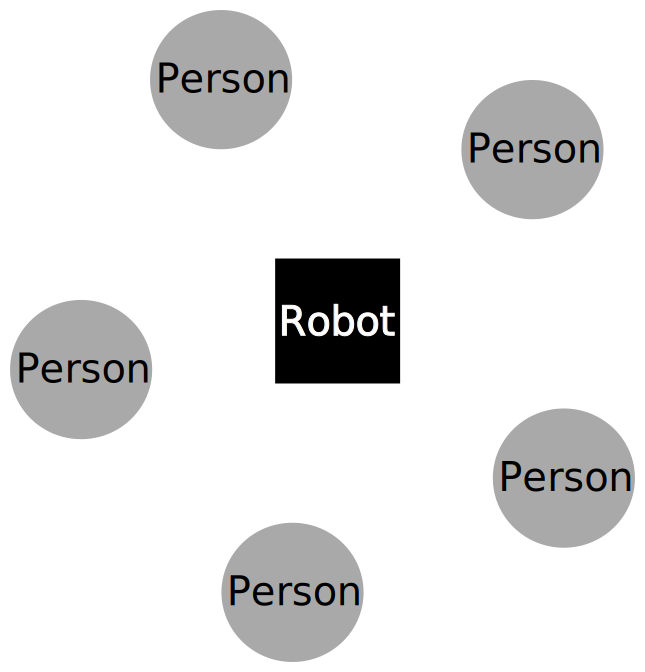
\includegraphics[width=0.5\columnwidth]{images/asrsetup.pdf}
	\caption{Speech recognition test: person setup around the robot for 2nd part.}
	\label{fig:asrsetup}
\end{figure}

% \subsection{Data recording}
% Please record the following data (See~\refsec{rule:datarecording}):
% \begin{itemize}
%     \item Audio
%     \item Commands
%     \item Images
% \end{itemize}

\subsection{Referee instructions}

The referee needs to
\begin{itemize}
    \item avoid shouting to the robot
    \item avoid getting closer to the robot (or even move)
    \item speak to the robot loud and clear with plain standard English
    \item avoid repeating questions for the same robot
    \item distribute the questions among the volunteers
\end{itemize}

\subsection{OC instructions}

\textbf{1 day before the test}
\begin{itemize}
    \item Provide the set of predefined questions
\end{itemize}

\textbf{2 hours before the test}
\begin{itemize}
    \item Announce the placement of the robots
    \item choose the volunteers for the second part of the test, and clearly explain the procedure to them.
    \item When the test is held outside the arena, announce the (way)point through which the robot shall leave
\end{itemize}

\subsection {Audio Data Recollection}
Teams are encouraged to submit to the TC the audio data recorded during the test, specially that which was captured during speech recoginition. If so, teams are urged to provide it with annotation of what the user said and what was recognized. Audio files are expected to be mono, one per microphone (in the case array recordings), of a sample rate equal to or higher than 16 kHz, and with a sample size of at least 16 bits. Depending on the quality of the recordings and their annothations, an official certificate that formalizes these efforts may be provided to submitting teams.

\newpage
\subsection{Score sheet}
The maximum time for this test is 5 minutes.

\begin{scorelist}

	\scoreheading{Crowd} % Max 15 points
	\scoreitem{ 5}{State crowd's size}
	\scoreitem{10}{State crowd's male/female count}

	\scoreheading{Riddle game} % Max 55 points
	\scoreitem[ 5]{5}{Understanding question}
	\scoreitem[ 5]{5}{Correctly answered a question}
	\scoreitem{ 5}{Answering all 5 riddle game question}

\ifDSPL{
	\scoreheading{[DSPL only] Blind man's bluff game} % Max 130
	\scoreitem[10]{ 5}{Understanding question on the first attempt}   % 50
	\scoreitem[10]{ 2}{Understanding question on the second attempt}  % -- (20)
	\scoreitem[10]{ 2}{Correctly answered a question}                 % 20
	\scoreitem[10]{ 5}{Turned towards person asking the question}     % 50
	\scoreitem{10}{Answering all 10 blind man's bluff questions}      % 10
}

\ifNotDSPL{
	\scoreheading{[OPL \& SSPL] Blind man's bluff game} % Max 130
	\scoreitem[ 5]{10}{Understanding question on the first attempt}   % 50
	\scoreitem[ 5]{ 5}{Understanding question on the second attempt}  % -- (25)
	\scoreitem[ 5]{ 5}{Correctly answered a question}                 % 25
	\scoreitem[ 5]{10}{Turned towards person asking the question}     % 50
	\scoreitem{ 5}{Answering all 5 blind man's bluff questions}       %  5	
}

	\setTotalScore{200}	
\end{scorelist}

\ifEvaluationSheet{
\textbf{Crowd setup ground truth}
\begin{figure}[!htb]
	\centering
	\begin{minipage}{.3\textwidth}
		\begin{center}
			\begin{tabular}{|l||l|l|l|l|}
				\hline
				Name & 
				\parbox[t]{2mm}{\rotatebox[origin=c]{90}{Stand}} & \parbox[t]{2mm}{\rotatebox[origin=c]{90}{Sit}} & \parbox[t]{2mm}{\rotatebox[origin=c]{90}{Lay}} & \parbox[t]{2mm}{\rotatebox[origin=c]{90}{Arm pose}}\\\hline
				× & × & × & × & ×\\\hline
				× & × & × & × & ×\\\hline
				× & × & × & × & ×\\\hline
				× & × & × & × & ×\\\hline
				× & × & × & × & ×\\\hline
				× & × & × & × & ×\\\hline
			\end{tabular}
		\end{center}
	\end{minipage}
	\begin{minipage}{.3\textwidth}
		\begin{center}
			\begin{tabular}{|l||l|l|l|l|}
				\hline
				Name & 
				\parbox[t]{2mm}{\rotatebox[origin=c]{90}{Stand}} & \parbox[t]{2mm}{\rotatebox[origin=c]{90}{Sit}} & \parbox[t]{2mm}{\rotatebox[origin=c]{90}{Lay}} & \parbox[t]{2mm}{\rotatebox[origin=c]{90}{Arm pose}}\\\hline
				× & × & × & × & ×\\\hline
				× & × & × & × & ×\\\hline
				× & × & × & × & ×\\\hline
				× & × & × & × & ×\\\hline
				× & × & × & × & ×\\\hline
				× & × & × & × & ×\\\hline
			\end{tabular}
		\end{center}
	\end{minipage}
	\begin{minipage}{.3\textwidth}
		\begin{center}
			\begin{tabular}{|l||l|l|l|l|}
				\hline
				Name & 
				\parbox[t]{2mm}{\rotatebox[origin=c]{90}{Stand}} & \parbox[t]{2mm}{\rotatebox[origin=c]{90}{Sit}} & \parbox[t]{2mm}{\rotatebox[origin=c]{90}{Lay}} & \parbox[t]{2mm}{\rotatebox[origin=c]{90}{Arm pose}}\\\hline
				× & × & × & × & ×\\\hline
				× & × & × & × & ×\\\hline
				× & × & × & × & ×\\\hline
				× & × & × & × & ×\\\hline
				× & × & × & × & ×\\\hline
				× & × & × & × & ×\\\hline
			\end{tabular}
		\end{center}
	\end{minipage}
\end{figure}
}{}
% Local Variables:
% TeX-master: "Rulebook"
% End:


% Local Variables:
% TeX-master: "Rulebook"
% End:


\newpage
\section{Help-me-carry}
The robot's owner went shopping for groceries and needs help carrying the groceries from the car into the home.

\subsection{Goal}
The robot must help bringing some objects into the arena from outside.

\subsection{Focus}
This test focuses on safe, robust navigation, people following and navigation in unknown environments.

\begin{itemize}[leftmargin=3cm]
  \item[DSPL \& OPL] Test focuses also in Object Detection and Manipulation.
  \item[SSPL] Test focuses also in People Detection and Human-Robot Interaction.
\end{itemize}

\subsection{Setup}
The operator (the robot's owner) has a set of bags (and possibly other objects) that need to be carried from a place outside the arena back inside.

\begin{enumerate}
  \item \textbf{Location:} One of the arenas (apartment) and its surroundings. The apartment is in its normal state. Part of the test is performed outside the arena in a public space.
  \item \textbf{Start:} The robot starts waiting inside the arena.
  \item \textbf{Car:} The car is any landmark chosen (but \emph{not} announced) beforehand outside the arena. Several bags (see~\refsec{rule:scenario_objects}) with groceries are located where the car is parked.
  \item \textbf{Doors:} All doors in the apartment are initially open.
  \item \textbf{Operator:} A \enquote{professional} operator is selected by the TC to act as the operator of the robot.
  \item \textbf{Uncontrolled environment:} There are no restrictions on other people walking by or standing around throughout the complete task.
\end{enumerate}

\subsection{Task}
\textbf{Remark:} Obstacles obstructing robot's path can be found anytime. See~\ref{sec:helpmecarry_obstacles} for details.
\begin{enumerate}
  \item \textbf{Start:} The robot starts at a designated starting position in the arena, and waits for the \textit{professional} operator. The operator steps in front of the robot and tells it to follow (e.g.~by saying \enquote{follow me}). The team is \emph{not} allowed to instruct the operator.

  \item \textbf{Memorizing the operator:} The robot has to memorize the operator. During this phase, the robot may instruct the operator to follow a certain setup procedure.

  \item \textbf{Following the operator:} When the robot signals that it is ready to start, the operator starts walking --in a natural way-- towards the car. Upon arrival, the operator will indicate the robot when they have reached their destination as instructed by the robot (e.g.~by saying \enquote{here is the car} or \enquote{stop following me}).

  \newcounter{enumTemp}
  \setcounter{enumTemp}{\theenumi}
  \item {[DSPL \& OPL]} \textbf{Bringing groceries in}
  The operator asks the robot to take a bag to a specific location (e.g.~\enquote{Take this bag to the kitchen table}).
  \begin{enumerate}
    \item \textbf{Bag pick-up:} The robots picks up the bag via natural handover (See remarks).
    \item \textbf{Bag delivery:} The robot takes the bag to the instructed destination. It may place the bag on the floor or onto the placement location.
    \item \textbf{Asking for help:} Close to the delivery location is another person. Facing that person, the robot must kindly request for help carrying groceries into the house.
  \end{enumerate}

  \setcounter{enumi}{\theenumTemp}
  \item {[SSPL only]} \textbf{Look for help} \\
  The robot is asked to find a person in a given room and ask them to assist carrying the groceries (e.g.~\enquote{Look for Louise in the Kitchen and ask her to help us}).
  \begin{enumerate}
    \item \textbf{Entering the house:} While on its way back to the house, the robot deals with different obstacles along it's path.
    \begin{itemize}[leftmargin=3cm]
      \item[\textbf{1st section}] While going back to the house, a person crosses robot's path.
      \item[\textbf{2nd section}] While going back, a person steps in front of the robot and asks it for the time.
    \end{itemize}

    \item \textbf{Find a person:} After reaching the designated room, the robot needs to find a person (there is only one person in the room, the name is meaningless).
  \end{enumerate}

  \item \textbf{Memorizing the \emph{new} operator:} The robot has to memorize the operator that will help. During this phase, the robot may instruct the operator to follow a certain setup procedure.

  \item \textbf{Guiding the operator:} When the robot signals that it is ready to start guiding, the robot guiding the operator to the car. The robot must clearly announce when the destination (the car) is reached.
  \begin{itemize}[leftmargin=3cm]
    \item[DSPL \& OPL] \textbf{Closed door:} Along it's path to the car, the robot will find a closed door (most likely the entrance to the house) that will need to be opened to reach the destination.
    \item[SSPL only] \textbf{Distracted operator:} After leaving the house, the operator is distracted by another person. The robot must re-gain the operator's attention, remind the task, and continue guiding the operator's to the car.
  \end{itemize}

\end{enumerate}

\subsection{Obstacles}
\label{sec:helpmecarry_obstacles}
Several obstacles are placed obstructing the robot's path. This can happen anytime and the robot has to react accordingly.
\begin{itemize}
  \item \textbf{3D Object:} A hard-to-perceive object
  % that requires more than a laser scanner to be detected
  (e.g.~coat rack, rolling chair, lamp, etc).

  \item \textbf{Small object:} Small object
  (e.g.~apple, glass, lego brick, etc).

  \item {[DSPL and OPL]} \textbf{Movable Object:} Something that can be moved or pushed away
  (e.g.~coat rack, rolling chair, lamp, etc).
  The robot must clearly state it is about to push the object.

  \item {[SSPL Only]} \textbf{\textit{Smart} obstacle:} A person to whom the robot may kindly ask to step aside.
  The person can be standing, lying, or sitting (chair or floor).
  The robot must look at the person and make clear who is interacting with.
\end{itemize}
%% Possible extensions:
%% - DONE: allow the operator to tell for each item where it should go
%% - At the destination room, there is a person waving, waiting for the robot to bring the items so (s)he can take them


\subsection{Additional rules and remarks}
\begin{enumerate}
  \begin{minipage}{0.65\textwidth}
  \item \textbf{Asking for passage:} The robot is allowed to (gently) ask individual people to step aside, but it is not allowed to blindly shout at groups of people.

  \item \textbf{Bag handles:} The handles of the bag are always clear and standing up. See Figure~\ref{fig:scenario_container_bag} in~\refsec{rule:scenario_objects} for bag description. \footnotemark

  \item \textbf{Bag pick-up:} The robot should actively try to grasp the bag from the operator's hand.
  If the robot can't take the bag from operator's hand (handover) it may request the operator to place or hang the bag on its manipulator, or place it on the floor for pickup.
  The robot must clearly state whether it has detected the operator's hand, bag release, etc.

  \item \textbf{Calling the operator back:} During the following phase, when the robot has lost the operator, it may call the operator back once.
  \end{minipage}\hfill%
  \begin{minipage}{0.65\textwidth}
  \end{minipage}\hfill
  \begin{minipage}{0.25\textwidth}
    \vspace{-20pt}
    \begin{figure}[H]
      \centering
      \includegraphics[width=2cm]{images/help_me_carry_bag.png}%
      \vspace{-10pt}
      %\caption{Example car with groceries.}
      \caption{Paper bag}
      \label{fig:help_me_carry_paper_bag}
    \end{figure}
    \vspace{-10pt}
    \begin{figure}[H]
      \centering
      \includegraphics[width=\textwidth]{images/help_me_carry_car.png}%
      \vspace{-20pt}
      %\caption{Example car with groceries.}
      \label{fig:help_me_carry_car}
      \caption{Car}
    \end{figure}
  \end{minipage}
  \item \textbf{Disturbances from outside:} If a person from the audience (severely) interferes with the robot in a way that makes it impossible to solve the task, the team may repeat the test immediately.

  \item \textbf{Groceries:} Any kind of objects can be found lying around the location designated as the \textit{Car}, such as boxes, sacs, plastic bags, crates, and the groceries itself to give realism to the test. Regardless what objects are present, the robot shall carry an \textbf{official shopping bag} as described below and in~\refsec{rule:scenario_objects}.

  \item \textbf{Instruction:} The robot interacts with the operator, not the team.

  \item \textbf{Natural walking:} The operator has to walk \enquote{naturally}, i.e., move forward facing forward. If not mentioned otherwise, the operator is not allowed to walk back, stand still, signal the robot or follow some re-calibration procedure.

  \item \textbf{Obstacle avoidance:} The robot is allowed to push (but not crush) the small object indefinitely without damaging it.
  Driving over, squeezing, crushing, breaking, etc., the small object immediately finishes the test.

  \item \textbf{Opening door:} If unable to open the door, the robot may ask the person being guided to open it (no points are scored).

\end{enumerate}
\footnotetext{This may change in the future. Then, a soft handle may be used which folds down}

% \subsection{Data recording}
%   Please record the following data (See~\refsec{rule:datarecording}):
% \begin{itemize}
%  \item Maps
%  \item Plans
% \end{itemize}

\subsection{Referee instructions}

The referee needs to
\begin{itemize}
  \item Distribute some objects over the shopping bags.
  \item Designate a few \enquote{car parking locations} from which the objects must be carried.
\end{itemize}

\subsection{OC instructions}

During setup days
\begin{itemize}
  \item Make bags available.
\end{itemize}

2 hours before the test
\begin{itemize}
  \item Announce the location in which robots will start.
  \item Get and instruct volunteers for the test.
\end{itemize}

\newpage
\subsection{Score sheet}
The maximum time for this test is 5 minutes.

{\footnotesize
\begin{scorelist}
	\scoreheading{Following Phase} % 30 pts
	\scoreitem{10}{Follow operator outside the arena}
	\scoreitem{15}{Follow operator to the car}
	\scoreitem{ 5}{Understand the destination}

\ifNotSSPL{
	% These are mutually exclusive, max score is thus 20
	\scoreheading{Bag pick-up (OPL \& DSPL only)}
	\scoreitem{+0}{Bag hanged. Gripper closes on timeout}
	\scoreitem{ 2}{Bag hanged. Gripper closes on hang}
	\scoreitem{ 5}{Pick up the bag from the floor}
	\scoreitem{10}{Scripted handover (hand/bag detection only)}
	\scoreitem{20}{Natural handover (active grasping + object release detection)}

	\scoreheading{DSPL \& OPL Tasks} % 80 pts
	\scoreitem{10}{Re-enter the arena}
	\scoreitem{ 5}{Deliver the bag at the specified location}
	\scoreitem{10}{Find the person at the specified location}
	\scoreitem{30}{Open door without help}
	\scoreitem{10}{Guide operator outside the arena}
	\scoreitem{15}{Guide operator to the car}
}

\ifSSPL{
	\scoreheading{SSPL only Tasks} % 100 pts
	\scoreitem{10}{Tell the time to the stranger}
	\scoreitem{30}{Re-enter the arena}
	\scoreitem{20}{Find the person at the specified room}
	\scoreitem{10}{Guide operator outside the arena}
	\scoreitem{30}{Guide operator to the car}
}

	\scoreheading{Obstacle avoidance} % 70 pts
	\scoreitem{20}{Avoiding small (box-sized) object}
	\scoreitem{20}{Avoiding 3D (hard-to-see) object}
\ifSSPL{%
	\scoreitem{30}{[SSPL] Asking a person to step aside (\textit{smart} obstacle)}
}%
\ifNotSSPL{%
	\scoreitem{30}{[DSPL \& OPL] Moving away movable object}
}%

	\setTotalScore{200}
\end{scorelist}
}

% Local Variables:
% TeX-master: "Rulebook"
% End:



\newpage
\section{General Purpose Service Robot}

%
% MAURICIO @2017
% Short instructions as in 2012 rulebook
%
This test evaluates the abilities of the robot that are required throughout the set of tests in stage I of this and previous years' RuleBooks. In this test the robot has to solve multiple tasks upon request. That is, the test is not incorporated into a (predefined) story and there is neither a predefined order of tasks nor a predefined set of actions. The actions that are to be carried out by the robot are chosen randomly by the referees from a larger set of actions. These actions are organized in three categories with different complexity. Scoring thereby depends on the complexity class.

%
% MAURICIO @2017
% Same focus as in 2012 rulebook. There should be no problem since this is SOLVED
%
\subsection{Focus}
This test particularly focuses on the following aspects:
\begin{itemize}
	\item No predefined order of actions to carry out (to get away from state machine-like behavior programming).
	\item Increased complexity in speech recognition.
	\item Environmental (high-level) reasoning.
	\item Efficient and fast task execution (speed).
\end{itemize}


%
% MAURICIO @2017
% Test has been shorten based in 2012 one, however, categories have changed
% to bypass NLP and avoid problems agreed by TC.
%
% All extra explanations have been sent to corresponding appendix.
%
\subsection{Task}

\begin{enumerate}
	\item \textbf{Entering and command retrieval:} The robot enters the arena and drives to a designated position where it has to wait for further commands.

	\item \textbf{Command generation:} A command is generated randomly, depending on the command category chosen by the team (see below). Commands are generated by the generator which is made publicly available at https://github.com/kyordhel/GPSRCmdGen. \\

	\item \textbf{Command categories:} The team may choose from the following three categories:
	\begin{enumerate}
		\item \textbf{Category I:} Tasks with a low difficulty degree.
		\item \textbf{Category II:} Tasks with a moderate difficulty degree.
		\item \textbf{Category III:} Tasks with a high difficulty degree or with incomplete/erroneous information.
	\end{enumerate}

	\item \textbf{Task assignment:} The robot is given the command by the operator and may directly start to work on the task assignment.

	\item \textbf{Returning to the operator:} After accomplishing the assigned task, the robot has to move back to the operator to retrieve the next command (i.e., go back to 1. without the need of re-entering the arena). The robot can work on at most three commands. After the third command, it has to leave the arena.

	\item \textbf{Exiting the arena:} After accomplishing the assigned task, the robot has to leave the arena.

	The robot must prove it has understood the given command by repeating it (Please see the remarks about this in section~\ref{sec:gpsr_remarks}).
\end{enumerate}

\subsection{Additional rules and remarks}
\label{sec:gpsr_remarks}
\begin{enumerate}
	\item \textbf{Referees:} Since the score system in this test involves a subjective evaluation of the robot's behavior, the referees are EC/TC members.

	\item \textbf{Category selection:} For every of the three commands given to the robot, the team chooses the desired command category.

	\item \textbf{Operator:}
	\begin{itemize}
		\item The person operating the robot is one of the referees (default operator).
		\item If the robot appears to consistently not be able to understand the operator, the referees ask the team to use a custom operator or bypassing speech recognition (\refsec{rule:asrcontinue}).
	\end{itemize}

	\item \textbf{Retrieving the command:} The robot must show it has understood the given command by repeating the command (i.e.~stating all the required information to accomplish the task).
	\\
	\textit{Note:} Referees must have sufficient evidence proving the robot is actively trying to execute the commanded tasks to score. Robots skipping command execution will not receive points for understanding the command.

	\item \textbf{Incremental scoring:} Scoring depends on the category chosen by the team leader and the previous successfully accomplished command. Thereby, scoring for a second and third command depends on how well the robot solved (not understood) a first and second command respectively. Referees determine how well the command was accomplished and its impact on the incremental scoring of subsequent commands.
\end{enumerate}

\subsection{Referee and OC instructions}
\textbf{2h before test:}
\begin{itemize}
	\item Specify and announce the entrance and exit door
	\item Specify and announce the command retrieval point
\end{itemize}

\subsection {Audio Data Recollection}
Teams are encouraged to submit to the TC the audio data recorded during the test, specially that which was captured during speech recoginition. If so, teams are urged to provide it with annotation of what the user said and what was recognized. Audio files are expected to be mono, one per microphone (in the case array recordings), of a sample rate equal to or higher than 16 kHz, and with a sample size of at least 16 bits. Depending on the quality of the recordings and their annothations, an official certificate that formalizes these efforts may be provided to submitting teams.

\newpage
\subsection{Score sheet}
\begin{scorelist}[timelimit=7]
	\scoreheading{Main Goal}
	\scoreitem[3]{80}{Understand the spoken command}
	\scoreitem[3]{100}{Demonstrate a plan has been generated}
	\scoreitem[3]{250}{Solving the command}
	
	\scoreheading{Bonus Rewards}
	\scoreitem{200}{Interleaved Task Bonus}

	\scoreheading{Penalties}
	\penaltyitem[3]{20}{Using a custom operator}
	\penaltyitem[6]{30}{Request a rephrasing}
	\penaltyitem[3]{50}{Bypassing speech recognition}
	\penaltyitem[3]{250}{Human assistance: will apply a percentage penalty according to similar penalties in other tests.}
\end{scorelist}




% Local Variables:
% TeX-master: "Rulebook"
% End:


\chapter{Tests in Stage II}
\label{chap:stage_II}

\begin{itshape}
All ability and integration tests in \iterm{Stage~II}  are performed only once. Some tests have optional tasks that grant additional points when performed correctly, clean and fast. The \iaterm{Technical Committee}{TC} must be informed if a team is planning to perform any of the optional tasks. Unless explicitly stated otherwise, no additional time is given while performing optional tasks.

In the \iterm{Open Challenge} the robot must be able to show to the \iaterm{Technical Committee}{TC} the achievements on the main research line of its own team. This test grants up to 250 points.

\section{Robot \& team cooperation}
We encourage robots and teams to work together when performing challenges.
For scoring, points are awarded per subtask. The robot (and thus team) performing the subtask gets the points.
For example, in the Restaurant-challenge, if one robot of team A can take the order and another robot of team B delivers the order, then the points for taking the order go to team A, while the points for delivering go to team B. 
Of course, team A \& B can both perform the challenge in their own turn.

\end{itshape}

\newpage
\section{Set a table and clean it up}

Setting up a table for a meal and cleaning it up afterwards is one of the most repetitive tasks in a household environment. How wonderful it would be to have a robot doing it for us. This tasks aims at evaluating the capability of robots at this task.

The task comprises two phases: in phase~I, the robot is asked to set up the table, according to an optional variation given by the referee, and in the phase~II, the robot is supposed to cleanup the table, returning all placed objects to their original location, including detecting and clearningspills with a cleaning cloth.

In phase~I, the operator requests the robot to setup the table for a meal. In this request, the operator may specify one variation of the meal, e.g., milk or coffee, bread or cookies. The robot should then set the table using items stored in various places of the kitchen, and afterwards it must clean it up, including small spills on the table. Some of the items are easly accessible (e.g., over the kitchen counter) while others may require the opening of doors (e.g., inside a cloret). Furthermore, some of these items may contrain the way they are handled by the robot (e.g., avoid pouring contents of a container). These items must be placed on a table reasonably following social conventions in terms of their positions on the table\footnote{Strict adherence to any social convention is out of the scope of the competition, and thus will not be evaluated.}. Midway during placement, the robot owner may change/adjust the position of some of the items; the robot is expected to handle appropriately the situation.

In phase~II, the operator requests the robot to clean up the table. This includes both returning the placed objects to their original location, and cleaning up dirt and spills using a cleaning cloth. This requires the robot ro memorize the location the objects were originally recognized.


\subsection{Example}

The operator requests the robot to set the table for breakfast. Then, the robot replies asking whether the operator prefers bread of cookies, to which the operator replies prefering bread.  Several items are placed on the table: a plate, cutlery, a cup, napkins, a basket with bread, a cereal box, etc. The basket with bread, a napkin, and the cereal box are on the kitchen counter; the plate, the cutlery, and the cup are inside a closet. The robot starts moving these items, one by one, from their original position to the table. Some of these objects pose specific challenges to robot manipulation: the napkin is a flexible object, the bread basket contains bread, thus the robot must hold it with care, the items inside the closet require the closet door to be opened, and the cutlery is non-trivial to grasp. After the bread basket is placed on the table, the robot owner decides to move its place, so the positioning of remaining objects must have this in consideration. Then the robot will await an instruction by the operator to clean up the table. While taking his/her meal, the table gets dirty with a spill. The robot must detect the spill and clean it up using a cleaning cloth. Then, all of the other items are returned to their original locations. The task concludes once the table returns to its original state.

\subsection{Goal}

The robot has to move a list of relevant objects, with a possible variation stated by the operator, onto the a predefined table in the kitchen. Then it should return all placed items to their original locations and cleanup dirt ansd spills from the table.

\subsection{Focus}

This test focuses on HRI, semantic mapping, object perception and manipulation.

\subsection{Setup}

Half of the objects are placed on the kitchen counter, while the remaining ones inside a predefined closet, which is closed before the robot entering the arena. The table should be initially cleared of any object. The robot will start at a predefined location, away from both the kitchen counter and the table. The team may optionally specify to the referees the variations supported by the robot, with at least two options. The referee then selects one of them randomly, not disclosing the choice.

\subsection{Task}
\label{sattu:task}

\begin{enumerate}
\item \textbf{Requesting the task:} The operator requests the robot to set up the table.
\item\label{sattu:s2} \textbf{Asking for variation:} (optional) The robot asks the operator for an option, to which the operator replies with the randomly selected (and undisclosed) option.
\item \textbf{Searching for objects:} The robot must detect which objects are missing on the table and search for them either on the kitchen counter on inside the closet.
\item \textbf{Grasping objects:} The robot must grasp any missing object and move it to the table.
\item \textbf{Placing objects:} Each object must be placed in a socially accepted position, not coliding with any object there.
\item \textbf{Changing objects position:} The operator will change the position of two objects on the table at any time, before the placement of the last one.
\item \textbf{Cleaning up the table:} After the meal, the operator requests the robot to clean up the table. The robot returns the objects to their original location, \textit{i.e.,} where they were found in the first place.
\item \textbf{Cleanup dirt and spills:} The robot must detect dirt and spills on the table and clean them up using a cleaning cloth.
\end{enumerate}

\subsection{Additional rules and remarks}
\begin{enumerate}
\item \textbf{No setup:} The robot must be ready to start the test with a voice command or start button when requested by the referee. There is no setup time.
\item \textbf{Startup:} The robot must be started with a single voice command or via a start button (Section \refsec{rule:start_signal}). If the robot is unable to start it must be removed immediately.
\item \textbf{Single try:} The robot must be able to start from the first attempt. 
`There is no restart for this test. If the robot is unable to start it must be removed immediately.
\item \textbf{Collisions:} Slightly touching the table.
  Driving over the objects or any other form of a major collision is not allowed, and the referees directly stop the robot (Section \refsec{rule:safetyfirst}).
\item \textbf{Object types:} The objects selected from the \textit{Standard Objects Set} will be chosen to be easily detectable and contrasting with the background (kitchen counter or closet). A maximum of 6 objects is considered for this task, where two of them is hard to grasp, e.g., cutlery, and another two must be handled upright, e.g., cup.
\item \textbf{Recognition report:} Robots must create a PDF report file including the list of recognized objects with a picture showing the object and the object name/label.
  This file may be stored on a USB-stick on the robot which is given to the TC after the test. The PDF file name should include the team name and a timestamp. 
  Furthermore, it must be unmistakeable which label belongs to which object. Objects must also be recognizable in the report by a human (TC) so that it can be scored. 
%  An overview of the shelf with bounding boxes and labels attached to the bounding boxes is handy for the TC to score.
False positives in the report (labeling an object which is not an object but e.g. the edge of the shelf) are penalized.
%\item \textbf{QR Codes:} The team may request to use a special set ob objects identified with QR codes if the robot is not able to correctly recognize the objects. The use of this special QR-object-set must be announced to the TC at least on hour before the test starts. When QR Codes are used, no points are given for object recognition.
\item \textbf{Clear area:} The robot may assume that there are no obstacles between the table, the kitchen counter, and the closet.
\item \textbf{Object list:} A total of 6 objects is considered, 3 of them considered easy to grasp (e.g., a cereal box, a cup, and a plate), while the remaining 3 hard to grasp (e.g., cutlery, napkins, and a basket with bread).
\item \textbf{Task variation:} The team may provide the referees a written set of options for setting up the table. These options must be written as possible answers to the robot question (step~\ref{sattu:s2} in section~\ref{sattu:task}). The correct execution of the specified variation should be clearly visible, e.g., choice of an object placed on the table.
\end{enumerate}

\subsection{Data recording}
  Please record the following data (See \refsec{rule:datarecording}):
  \begin{itemize}
   \item Images of recognized objects
   \item List of moved items
  \end{itemize}

\subsection{Referee instructions}

The referee needs to
\begin{itemize}
\item Clean up any remaining object on the table.
\item Place the objects on either the kitchen counter or inside the closet, half of them in each one of these two locations. Each one of these locations must contain at least one easy to grasp and one hard to grasp object.
\item Close the closet door.
\item Ask the team whether they implemented a meal variation, and if yes, choose randomly one of the options, not disclosing the choice.
\end{itemize}

\subsection{Score sheet}

The maximum time for this test is \textbf{10 minutes}. A maximum of 6 objects is
considered in this scoresheet.

\begin{scorelist}
% Grasp (any object): 10
% Place (anywhere in the cupboard): 10
% Place in correct place: 15
% Recognize known object correctly (without grasping/placing something of that class): 10
% Label two unknown objects of the same class with the same label (e.g. ``class0''): 15

% Place known object near known object of same class: 40
% Place unknown object near unknown object of the same class: 50

  \scoreheading{Meal variation}
  \scoreitem[1]{10}{For asking for the meal variation and confirming the choice}

	\scoreheading{Grasping objects}
	\scoreitem[12]{10}{For each successful grasp of any object (lifting it up to at least 5 cm for more than 10 seconds)}
	\scoreitem[12]{20}{For each successful grasp of an hard to
          grasp object (lifting it up to at least 5 cm for more than
          10 seconds)}

	\scoreheading{Placing objects}
	\scoreitem[6]{10}{For each successful placement of any object anywhere on the table (safely stands still for more than 10 seconds)}
	\scoreitem[6]{20}{For each successful placement of an hard to
          grasp object anywhere on the table (safely stands still for
          more than 10 seconds)}
        \scoreitem[1]{100}{For appropriately executing the operator's choice}
	\scoreitem[6]{-5}{For each collision of an object with another
        one on the table}

      \scoreheading{Cleaning up the  table}
	\scoreitem[6]{10}{For each successful placement of any object
          to its original location}
	\scoreitem[6]{20}{For each successful placement of an hard to
          grasp object to its original location(safely stands still for
          more than 10 seconds)}
        \scoreitem[1]{100}{For successfully cleaning up dirt and spill on
          the table}

	\scoreheading{Recognizing objects}
	\scoreitem[6]{10}{Every correctly recognized known object in the report file}
	% ??? \scoreitem[5]{15}{Every correctly label 2 unknown objects of the same class with the same label in the report file}
	\scoreitem[6]{-5}{False positive label}
	
% 	\scoreheading{Total task}
% 	\scoreitem[5]{40}{Place known object near known object of same class}
% 	\scoreitem[5]{50}{Place unknown object near unknown object of same class}

	\scoreheading{Penalty}
	\scoreitem[6]{-15}{Require a human to open the closet door}  % Or make this a bonus, but then there is a time issue as opening the door takes time. I think a penalty provides a better incentive

	% (+ 10 (* 12 (+ 10 20)) (* 6 (+ 10 20)) 100 (* 6 (+ 10 20)) 100 (* 6 10))
	\setTotalScore{990}
\end{scorelist}

% \subsection{Score examples} 

% TODO

% \begin{itemize}
%  \item Robot A fails at all manipulation attemps but makes an excelent report, with the 5 known objects labeled correctly and the 5 pairs of unknown objects correctly, will get 
% $5*10 + 5*15 = 125$ points. 
%  \item Robot B that fails to recognize anything but does move all the objects from the table to anywhere in the cupboard receives $5*10 + 5*10 = 100$ points.
%  \item Robot C grasps a single unknown item (``Cookies''), places it at the correct position near the other ``Cookies'' and also makes the same excelent report as robot A will get 
% 10 points for grasping, 10 foor placing anywhere and an additional 5 for placing at the right location, so 25 for that single object.
% The  total for robot C is then 150 points.
% \end{itemize} 


% Local Variables:
% TeX-master: "Rulebook"
% End:


% Local Variables:
% TeX-master: "Rulebook"
% End:


\newpage
\section{Tour guide [SSPL only]}
The robot guides spectators to the audience area and answer their questions after explaining what's @Home about.

\subsection{Focus}
This test focuses in safe outdoor navigation, people detection, gesture recognition, unconstrained natural language processing, and Human-Robot Interaction

\subsection{Setup}
\begin{itemize}
	\item \textbf{Location:} This test takes place outside the arena in a public space close to the @Home area.

	\item \textbf{Other people:} There are no restrictions on other people walking by or standing around throughout the complete task.

	\item \textbf{In Parallel:} This test can run in parallel, with several teams tested simultaneously.
\end{itemize}

\subsection{Task}

\begin{enumerate}
	\item \textbf{Start:} The robot waits at a designated starting position for the referee to give the start signal. When the referees start the time, the team is allowed to (briefly) provide some remarks about the robot's operation. After the instruction, the referee gives the start signal to the robot.\\

	\item \textbf{Finding spectators:} The robot starts moving to an open area and looks for (preferably large) groups of people. Once located the robot must approach to the spectators while calling for their attention in a \emph{friendly} way.\\

	People trying to call the attention of the robot (e.g.~by waving or shouting) have priority over those just walking by despite the number of the crowd. The robot may also approach to a single person.\\

	\item \textbf{Greeting an spectator:} Once the robot has gained the attention of the spectators, it must introduce itself (i.e.~saying it's name), and greet one of the spectators as customary in the venue's country (e.g.~bowing, handshaking, waving, etc).\\

	Note that all spectators may also want to greet the robot. The robot is expected to be polite and continue greeting on demand.\\

	\item \textbf{Guiding the spectators:} The robot must gently ask the spectators to follow it to any of the @Home audience areas and guide them there. Should the people not be willing to follow the robot, it must thank them and start looking for another group of spectators.\\

	\item \textbf{Explaining the league:} Once at the @Home audience area, the robot must ask the spectators to take seat. The robot proceeds to \textit{briefly} introduce RoboCup@Home and explain the Social Standard Platform League's objectives. \\

	\item \textbf{Answering questions:} At the end of the speech, the robot asks for questions from the spectators regarding what it just explained, answering at least two of them. The robot is allowed to rephrase questions before answering them.\\

\end{enumerate}

\subsection{Additional rules and remarks}
\begin{enumerate}
	\item \textbf{Safety First!} The robot will be stop at the slightest possibility of a human being harmed or molested. The robot must not force interaction with humans, nor scare them or make them feel uncomfortable. \\

	\item \textbf{Referee guard:} During the entire test, a referee will be following the robot from behind for keeping people safe and for scoring purposes.\\

	\item \textbf{Approaching to spectators:} When approaching to people the robot should act in a natural way by reducing its velocity as it approaches to the people. The robot must look safe and friendly.\\

	Shall the people flee, the robot must not chase them.\\

	\item \textbf{Spectators:} Spectators are people attending to the venue to see the competition with no restriction of any kind, therefore, their numbers, grouping, and behaviour are not controlled by the league. Were the case of no spectators available, volunteers can be used instead.\\

	\item \textbf{Bilingual robots:} Robots are allowed (and encouraged) to interact with people in a language other than English. In such cases, the robot must utter the English equivalent right after synthesising the localized sentence. \\

	Notice that spectators may prefer to ask questions in their native language when interacting with a bilingual robot. In such cases, the robot must translate the question for the Referee to understand it and answer the question in both languages.\\

	\item \textbf{Handshaking:} When handshaking, the robot must stay at a safe distance from the people (e.g.~about 1.5m) and reach out its \textit{hand}, but it must be a human, not the robot, who accepts and completes the handshake. If the human refuses to shake hands, the robot must retreat its manipulator immediately.\\

	\item \textbf{Disturbances from outside:} If a person from the audience (severely) interferes with the robot in a way that makes it impossible to solve the task, the team may repeat the test immediately.\\

	\item \textbf{Show must go on:} If the robot has engaged with a group of spectators when the allotted time for the test elapses, the robot is allowed to continue and finish the demonstration. However, no points are scored once the test is over.
\end{enumerate}

\subsection{Referee instructions}

The referees need to
\begin{itemize}
	\item Follow the robot at any time.
	\item Immediately stops the robot when considered necessary.
	\item Verify that the given answers are correct.
\end{itemize}

\subsection{OC instructions}

2h before test:
\begin{itemize}
	\item Recruit volunteers for the test (just in case).
	\item Announce the Start Location for the robots.
\end{itemize}

During the test:
\begin{itemize}
	\item Keep at least one area free in the audience area for robots to perform there.
	\item Send volunteers to join the Q\&A session to ask questions if necessary.
\end{itemize}

\newpage
\subsection{Score sheet}
The maximum time for this test is \textbf{10 minutes}.

\begin{scorelist}
	\scoreheading{Engaging spectators} % Max 50
	\scoreitem{30}{Find an spectator (or group)}
	\scoreitem{20}{Greet an spectator (handshake)}
	\scoreitem{10}{Greet and get greet by an spectator (bowing or waving)}

	\scoreheading{Guiding spectators} % Max 50
	\scoreitem{10}{Convince spectator to follow}
	\scoreitem{40}{Reach the audience area}

	\scoreheading{Q\&A Session} % Max 210
	% \scoreitem{10}{Finish talk without loosing spectators attention}
	\scoreitem{10}{Finish talk without loosing spectators}
	\scoreitem[2]{70}{Each correctly understood question}
	\scoreitem[2]{30}{Each correctly answered question}
	
	\scoreheading{Bilingual interaction} % Max 80
	\scoreitem{10}{Bilingual engaging}
	\scoreitem[2]{25}{Questions in $3^{rd}$ language}
	\scoreitem[2]{10}{Question answered also in $3^{rd}$ language}
	
	\setTotalScore{390}
\end{scorelist}


% Local Variables:
% TeX-master: "Rulebook"
% End:


\newpage
\newcommand{\bonusRobotCoop}{50~}

\section{Open Challenge}
\label{sec:test_open_challenge}

During the Open Challenge teams are encouraged to demonstrate recent research results and the best of the robots' abilities. It focuses on the demonstration of new approaches/applications, human-robot interaction and scientific value.

\subsection{Task}

The Open Challenge consists of a demonstration and an interview part.
It is an open demonstration which means that the teams may demonstrate anything they like.
The performance of the teams is evaluated by a jury consisting of all team leaders, TC and EC.
\OpenDemonstrationTask{seven}{three}

\subsection{Presentation}
During the demonstration, the team can present the addressed problem and the demonstrated approach.
\begin{itemize}
	\item A video projector or screen, if available, may be used to present a brief (max. 2 minute) presentation relevant to the demonstration.
	\item Teams may omit the video, use a more brief video, or have the robot act over the video in order to make more time for the robot demo.
	\item There may be no human presenter. This is intended to be a demonstration of the robot's capabilities and not a research talk. The robot may present for itself (e.g., describing what it is doing or providing a narrative for the presentation on its own).
	\item Humans may interact with the robot during the interaction, but are not to act as presenters. This judgement is left to the jury.
	\item The team can also visualize robot's internals, e.g., percepts.
\end{itemize}

It is important to note that the jury may decide to end the demonstration if there is nothing happening or nothing \emph{new} is happening.

\OpenDemonstrationChanges

\subsection{Jury evaluation}
\begin{enumerate}
	\item \textbf{Jury of team leaders:} All teams have to provide \emph{one} person
	(preferably the team-leader) to follow and evaluate the entire Open Challenge.
	\item \textbf{Evaluation:} Both the demonstration of the robot(s), and the answers of the team in the interview part are evaluated.\\
	For each of the following \emph{evaluation criteria}, each jury member submits a score from $0-100$:
	\begin{enumerate}
	\item Novelty and (scientific) contribution
	\item Difficulty level of the demonstrated task
	\item Success of the demonstration
	\item Overall (demo was convincing, fluent, interesting, etc.)
	\end{enumerate}
	A jury member is not allowed to evaluate and give points for the own team.
	\item \textbf{Normalization and outliers}:
	\begin{enumerate}
		\item The points given by each jury member are scaled to obtain a score from $0.0-1.0$.
		\item The normalized total score for each team is the mean of the jury member scores.
			To neglect outliers, the $N$ best and worst scores are left out:
			$$\mbox{score}_{norm} = \frac{\sum\mbox{team-leader-score}}{\mbox{number-of-teams} - (2N+1)}\times\frac{1}{100},
			\quad N=\begin{cases}2, & \mbox{number-of-teams} \ge 10\\1, & \mbox{number-of-teams} < 10 \end{cases}$$
		\end{enumerate}
		\item The final Open Challenge score for each team is computed at the end of Stage 2. The Open Challenge \scoring{final score} is the product of the normalized score multipled by the highest score achieved in Stage 2:
		$$\mbox{score} = \mbox{score}_{norm} \times \frac{min\Big(250, max\big(\{S_2\}\big)\Big)}{250},
		\quad \{S_2\}=\mbox{All Stage2 scores}
		$$
\end{enumerate}

\subsection{Additional rules and remarks}
\begin{enumerate}
	\item \textbf{Start signal:} There is no standard start-signal for this test.
	\item \textbf{Abort on request:} At any time during the demonstration, the jury may interrupt and abort the demonstration:
	\begin{enumerate}
		\item if nothing is shown: in case of longer delays (more than one minute), e.g., when the robot does not start or when it got stuck;
		\item if nothing new is shown: the demonstrated abilities were already shown in previous tests (to avoid dull demonstrations and push teams to present novel ideas).
	\end{enumerate}
\end{enumerate}

\subsubsection{Team-team-interaction:}
\label{rule:OC-team-team-interaction}
An extra bonus of up to \bonusRobotCoop points can be earned if robots from two teams (4 robots maximum, 2 from each team) successfully collaborate (robot-robot interaction).
\begin{enumerate}
	\item This bonus is earned for both teams.
	\item The robot(s) of the other team must only play a minor role in the total demonstration.
	\item It must be made clear that the demonstrations from the two teams are not similar, otherwise the points cannot be awarded.
	\item In case a team receives two (or more) bonuses, the maximum bonus will be taken.
	\item The collaboration is possible even if one of the two teams has not reached Stage 2.
	\item A team not participating in Stage 2 receives no bonus points for this test.
\end{enumerate}

\paragraph*{Inter-league collaboration}:
\label{rule:OC-inter-league-collaboration}
Inter-league collaboration must be announced to the OC at least one day before the test. Teams participating in multiple @Home Leagues does receive no bonus for cooperation. Standard Platform robots are allowed to take part in the Open Challenge of the Open Platform League, but Open Platform robots can \emph{not} participate in any Standard Platform League's test. In the same sense, DSPL robots are not allowed in SSPL and vice versa.

For sake of clarity, please consider the following example: Let be A, B two teams participating in RoboCup @Home where
\begin{itemize}
	\item Team A participates in SSPL.
	\item Team B participates in both SSPL and OPL.
	\item Team A and B have qualified into Stage II.
\end{itemize}
Then, by applying the \textit{Inter-league collaboration Rule} (See~\refsec{rule:OC-inter-league-collaboration}) the following statements can be concluded:
\begin{itemize}
	\item B OPL can not participate in A SSPL's open challenge.
	\item B OPL can not participate in B SSPL's open challenge.
	\item A SSPL can participate in B OPL's open challenge. Team A and B get a bonus because A <> B.
	\item B SSPL can participate in B OPL's open challenge. There is no bonus because B = B.
\end{itemize}




% Local Variables:
% TeX-master: "Rulebook"
% End:


\newpage
\section{Restaurant}
The robots are tested in a real environment such as a real restaurant or a shopping mall.
There are \emph{two} robots helping clients in the restaurant at the same time.

\subsection{Focus}
This test focuses on online mapping, safe navigation in previously unknown environments, gesture detection, human-robot interaction, and manipulation in a real environment.

The robot will need to create its own map from the environment and then move within it to handle human requests, such as delivering drinks or snacks, while people are walking around.
As this test is performed with 2 robots (2 teams, each with their own 1 robot) in parallel, the robots will also have to avoid each other.

\subsection{Setup}
\begin{enumerate}
	\item \textbf{Location:} A real restaurant fully equipped with a \enquote{Professional Barman} i.e.~the operator and at least three tables with \enquote{Professional Clients}.
\end{enumerate}

\subsection{Task}
\begin{enumerate}
	\item \textbf{Start:} The robot starts at a designated starting position. After the start signal is given, the robot may look around to keep an \textit{eye} on the tables.
	  The location of the tables is not taught to the robot via some training phase.

	\item \textbf{Calling:} A guest will ask for the robot's attention by waving \emph{and} calling it out using voice.
	  The robot must state out loud that it has detected the call.
	  % A robot must also indicate roughly where it has detected the call (e.g.~\enquote{to my left})
	  In case both robots notice the same call, the \textit{Professional Barman} will tell one of the robots to take the order.
	  The barman will say the robot's name followed by \enquote{Take the order} e.g.~\enquote{R2D2, take the order}.
	  The other robot will simply have to wait for another call.
	  If the robot \textit{not} commanded to take the order still goes, it will be commanded to wait (e.g.~\enquote{C3PO, Wait}).
	  In case the robot keeps going after that, the emergency button will be used to stop the robot.

% 	\item \textbf{Parallel orders:} It may occur that two guests want to order something at the same time and thus wave at the same time.
% 	  The referees will arange these two guests such that each is clearly visible to (in front of) one of the robots.

	\item \textbf{Ordering}: The robot must ask the person what he or she wants to order. See Orders below for details about ordering.
	\item \textbf{Avoiding random person:} At any time while going to any of the tables or to the \textit{Kitchen}, a person may step on the robot's path.
	  It is expected of the robot to avoid that person or stop and wait for it to move away.

	\item \textbf{Delivering phase:}
	\begin{enumerate}
		\item \textbf{Repeating the order:} Once again in the kitchen, the robot recites the orders for each table (e.g.~\textit{\enquote{Hamburger with fries for table A and Orange juice for table B}}, to the \textit{Professional Barman}.
		  The \textit{Professional Barman} will serve the order and place it into a tray on the Kitchen-bar.
		  If the barman cannot understand the order that the robot repeats, he cannot hand out the order and no points can be awarded for reciting the order.

		\item \textbf{Grabbing a beverage:} The robot must grab a can of the appropriate drink from a set of cans on the Kitchen-bar.

		\item \textbf{Grabbing a combo:}  The robot must carry a tray with the ordering from the kitchen-bar.
		Teams must indicate beforehand whether the robot is able to grasp the plate itself, whether it needs a tray or whether the plate needs to be handed to the robot.

		\item \textbf{Delivery:} The robot must place the order on the table.
		If the robot is not able to do this, the robot is allowed to hand over the order, but the client is not allowed to shift his/her chair or stand up.
		The robot must help the client, not the other way around.
	\end{enumerate}

	\item \textbf{Next customer, please:} When the robot is in the kitchen, the \textit{Professional Barman} will ask the robot to either find a new client to serve or to stop the test.
	The barman will either tell the robot \enquote{R2D2, Wait} to make it wait for another client or \enquote{R2D2, Stop the test} to end the test for that robot.
\end{enumerate}

\textbf{Orders:} The menu offers Beverages and Combos. An order may be a Beverage or Combo. Some guest(s) will order a Combo while another will order a Beverage.
  A Combo is a combination of two of the food items from the set of objects~\ref{rule:scenario_objects}, e.g.~\enquote{noodles with peanuts} or \enquote{noodles and peanuts}.
  Guests also prefer to state their order in a natural way, as they would in a restaurant operated by humans.

\begin{figure}[tbp]
	\centering
	\includegraphics[width=0.5\columnwidth]{images/restaurant.png}
	\caption{Restaurant test: example setup.}
	\label{fig:restaurant}
\end{figure}

\subsection{Additional rules and remarks}

\begin{itemize}
	\item \textbf{Safety!} This test takes place in a public area. That is, there may be people standing, sitting or walking around the area throughout the test. The robot is expected to not even slightly touch anything and is immediately stopped in case of danger.

	\item \textbf{Referees and guidance:} For safety reasons, the referees in this test are TC members. One of the referees follows the robot and is always in reach of the emergency button.

	\item \textbf{Start:} There is no fixed start signal in this test, it starts when both robots are ready (though within a reasonable time).

	\item \textbf{Order:} The way the user provides information to the robot is up to the robot's team. A natural interaction is preferred.

	\item \textbf{Location:} This test can be arranged in any real restaurant or shopping mall. If this is not possible, the test can be conducted in an arbitrary room containing the appropriate locations.
	  The only requirement is that this room is not part of the arena and that the teams do not know the room beforehand.
	  The exact location, including the object and delivery locations, will be defined by the technical committee on site (and in corporation with the local organization).
	  In addition, to avoid unnecessary time investment for navigation, the distances between tables and the \enquote{Kitchen Bar} will be minimal.

	\item \textbf{Disturbances from outside:} If a person from the audience (severely) interferes with the robot in a way that makes it impossible to solve the task, the teams may repeat the test immediately.

	\item \textbf{Learning tables:} Of course, it can only be sure that a robot correctly remembered where an order is suppposed to be delivered when it is able to go there after grabbing the order.

	\item \textbf{Instruction:} The robot interacts with the operators, not the team. That is, the team is only allowed to (very!) briefly instruct the \textit{Professional Barman}
	\begin{itemize}
		\item How to the tell the robot the order has been served
	\end{itemize}
	It is not allowed to the team to instruct the clients on how to get robot's attention. It shall be done in a natural way like when interacting with a human waiter.

	\item \textbf{Kitchen-bar:} The \textit{Kitchen-bar} will be a table located at the restaurant's kitchen, next to the place where the robot started.
	The robot may ask on which side of the robot the Kitchen-bar is, e.g.~on its left or right side. It may ask this at any time, but it is better if the robot infers this itself.
	It has the following setup.
	\begin{itemize}
		\item \textbf{Barman:} A \textit{Professional Barman} (member of the TC) will be at the other side of the Kitchen-bar to take the order provided by the robot and serve it in the official tray.
		\item \textbf{Beverages:} Beverages will be located on the Kitchen-bar next to the \textit{Professional Barman}.
	\end{itemize}

\end{itemize}

% \subsection{Data recording}
%   Please record the following data (See~\refsec{rule:datarecording}):
%   \begin{itemize}
%    \item Audio
%    \item Commands
%    \item Mapping data
%    \item Images
%    \item Plans
%   \end{itemize}

\subsubsection{Referee instructions}

The referee needs to
\begin{itemize}
  \item Prepare orders for each client in advance, so that there can be no confusion. These orders must also be available at the kitchen.
\end{itemize}

% \subsubsection{OC instructions}

% \textbf{2 hours before the test}
% \begin{itemize}
% \item
% \item
% \end{itemize}
% \textbf{During the test}
% \begin{itemize}
% \item
% \item
% \end{itemize}

\newpage
\subsection{Score sheet}
The maximum time for this test is 15 minutes.

\small\begin{scorelist}
	\scoreheading{Main Goal}
	\scoreitem[2]{500}{Complete an order}

	\scoreheading{Bonus rewards}
	\scoreitem{75}{Detect calling or waving guest}
	\scoreitem{75}{Arrive at table of calling or waving guest without guidance}
\end{scorelist}

% Local Variables:
% TeX-master: "Rulebook"
% End:


% Local Variables:
% TeX-master: "Rulebook"
% End:


\newpage
%%%%%%%%%%%%%%%%%%%%%%%%%%%%%%%%%%%%%%%%%%%%%%%%%%%%%%%%%%%%%%%%%%%%%%%%%%%%%
%
% EEGPSR
%
%%%%%%%%%%%%%%%%%%%%%%%%%%%%%%%%%%%%%%%%%%%%%%%%%%%%%%%%%%%%%%%%%%%%%%%%%%%%%

% Number of concurrent teams
\newcommand{\eegpsrTeams}{2~}
% Maximum number of commands to be given to a robot
\newcommand{\eegpsrMaxCmd}{3~}
% Maximum amount of time given to a team to perform a single command
\newcommand{\eegpsrMaxCmdTime}{5~}
% Maximum amount of time given to a team to perform all commands
\newcommand{\eegpsrMaxTeamTime}{\eegpsrMaxCmd$\times$\eegpsrMaxCmdTime}

\section[EEGPSR]{E\textsuperscript{2}GPSR \\ \normalsize{(Enhanced Endurance General Purpose Service Robot)}}
\label{sec:eegpsr}

This test evaluates the abilities of the robot that are required throughout the set of tests in stages I and II of this (2016) and previous years. In this test the robot has to solve multiple tasks upon request over an extended period of time (30-45 minutes). That is, the test is not incorporated into a (predefined) story and there is neither a predefined order of tasks nor a predefined set of actions. The actions that are to be carried out by the robot are chosen randomly by the referees from a larger set of actions. These actions are organized in three categories with different, incremental, complexity. Scoring thereby depends on the complexity class.

\subsection{Focus}
This test particularly focuses on the following aspects:
\begin{itemize}
	\item No predefined order of actions to carry out (to get away from state machine-like behavior programming).

	\item Increased complexity in speech recognition (possible commands are less restricted in both actions/operators and arguments/objects, commands can include an object and a location, e.g., \quotes{put the apple on the kitchen table}).

	\item More advanced capabilities (e.g. activity detection, unknown object description, pouring, manipulating tray, etc.).

	\item Environmental (high-level) reasoning, including:
  \begin{itemize}
	\item Memory (robot must remember performed actions, e.g. ``where did I leave this thing I grabbed earlier'')
	\item Awareness (events may occur while the robot is waiting for a command).
  \end{itemize}

  \item Robust long-term operation.

\end{itemize}

\subsection{Task}

\begin{enumerate}
	\item \textbf{Entering and command retrieval:} The robot enters the arena and drives to a designated position where it has to wait for further commands. \\

	\item \textbf{Command generation:} A command is generated randomly depending on the abilities chosen by the team (see \refsec{sec:eegpsr-abilities}) and those which haven't been evaluated yet. The command is composed by up to three actions that the robot has to show it has recognized. The robot may repeat the understood command and ask for confirmation. If it can't recognize the command correctly, it can also ask the speaker to repeat the whole command again.

	The command may not include all the information being necessary to accomplish the task. In those cases, the robot can ask a question to retrieve the missing information about the task, but is not required to. In the questions the robot has to make clear what it has already understood, e.g., tell the operator that it has understood to bring a particular beverage can, but not where can is located in the arena. The robot may also simply start searching. \\

	Each new generated command may require information from the previously given ones. Also, the difficulty of the new commands will be increased with respect of the previously generated ones. \\

	\item \textbf{Task assignment:} The robot is given a command by the operator and may directly start to work on the task assignment. If a robot is unable to perform a command, it should get back to the operator, and clearly state \textbf{why} it wasn't able to accomplish the task. \\

	\item \textbf{Answering questions:} After the first command has been (partially) accomplished, the operator may ask the robot to provide information about its actions and the environment, such as: what the robot has just accomplished, the location of a person or object, number of people in a given room, the state of a door, what the robot is holding, etc. \\

	\item \textbf{Task execution:} The robot must stop the execution of a task and return to its designated position within \eegpsrMaxCmdTime minutes. Otherwise the robot must be moved to its designated position immediately. If a restart is still available to the team, it can be restarted at the designated position. \\

	\item \textbf{Returning:} After accomplishing the assigned task, the robot has to move back to its designated position to wait and retrieve the next command (i.e., go back to 1. without the need of re-entering the arena). The robot can work on at most \eegpsrMaxCmd commands. \\

	\item \textbf{Timing:} The total time allotted to the robot for command retrieval and task execution is \eegpsrMaxTeamTime minutes. If the robot is not at its designated position after the time has expired, it must be moved at its designated position immediately. See the section on scheduling below as well.\\

	\item \textbf{Exiting the arena:} When commanded to do so, a robot should leave the arena. \\

\end{enumerate}

\subsection{Tested abilities \& scoring}
\label{sec:eegpsr-abilities}
Each commanded action involves at least one of the following abilities. During the test, all the abilities listed are evaluated. Completing a command within time 

The following abilities will be scored considering the best execution only (e.g.~successfully grasping scores for \textit{grasping}).

\begin{itemize}
	\item Advanced manipulation (pouring, placing in a box, transporting a tray, etc.).
	\item Awareness (see \refsec{sec:eegpsr-awarenes}).
	\item Complex command understanding (natural language).
	\item Count people / objects in a given location.
	\item Feature recognition (color, gender, gesture, pose, size, etc.).
	\item Gesture recognition.
	\item Object grasping.
	\item Object placing.
	\item Object recognition.
	\item People finding / learning / recognizing.
	\item People following / guiding.
	\item Speech recognition.
	\item Memory and answering questions.
\end{itemize}

The following abilities will be scored considering the worst execution only (e.g.~colliding once negates all previous scoring achieved for \textit{navigation}):

\begin{itemize}
	\item Collision-free navigation.
\end{itemize}


The team may choose to be evaluated in the following abilities (one try only):
\begin{itemize}
	\item Activity detection (waking up, reading, dancing, etc.).
	\item Natural handover (take / give).
	\item Open a door/drawer.
	\item Unknown object description / recognition.
\end{itemize}

\subsection{Awareness}
\label{sec:eegpsr-awarenes}
Either, while the robot is executing a task or while the robot is waiting for a command, an \textit{unexpected} event may occur, having the robot to \textbf{properly identify it} and react to it.

These \textit{unexpected} events will only occur within the field of view of the robot, and include:
\begin{itemize}
	\item \textbf{Waving:} The operator waves to the robot expecting the robot to approach to them, prior to give a command.
	\item \textbf{Falling down:} The person being followed by the robot suddenly falls down, robot must offer assistance.
	\item \textbf{Walking away:} One of the people in the crowd being counted suddenly leaves the room. The robot must indicate thi clearly somehow. 
	\item \textbf{Door shutting:} A door is suddenly shut while the robot is on its way to it.
\end{itemize}

\paragraph*{Remark:} for security concerns, team must notify the referees when the robot lacks of awareness.

\subsection{Additional rules and remarks}
\label{sec:eegpsr-remarks}
\begin{enumerate}
	\item \textbf{CONTINUE rule:} Teams are able to use the CONTINUE rule in this test, with all the standard penalties it involves as described in section \refsec{rule:asrcontinue}.
	%The CONTINUE rule can only be used with the custom operator (e.g. both penalties of custom speaker and CONTINUE rule will be applied). \\

	\item \textbf{Number of Teams and Scheduling:} In each test slot multiple teams (preferably \eegpsrTeams teams) may be competing in the arena concurrently. The robots will be tested in an interleaved fashion: The robots will retrieve commands and execute the task one after the other. As stated above, each robot will have a maximum amount of \eegpsrMaxCmdTime minutes per command (including time for retrieving the command and executing it). \\
	
	\item \textbf{Returning to designated position:} To facilitate a fluent and untroubled performance of the robots, they must return (or being returned) to their designated position before the \eegpsrMaxCmdTime minutes command time elapses. \textbf{If a robot moves from its designated position while another robot is working on a command, it must be immediately disabled} and moved to its designated position. If a restart is still available to the team, it can be restarted at its designated position. \\

	\item \textbf{Carrying robots:}	To carry the robot, at most two team members are allowed in the arena, and the robot must be moved as quickly as possible. To start or restart the robot, at most one team member may operate the robot. The team members moving and operating the robots must leave the arena immediately after the robot is placed or started. \\

	\item \textbf{Referees:} Since the score system in this test involves some subjective criteria while evaluating the robot's behavior, the referees are EC/TC members. One referee is assigned to each team to judge performance, to measure the time for working on a command, and to keep track of the overall operating time of the robot. \\

	\item \textbf{Operator:}
	\begin{itemize}
		\item The person operating the robot is one of the referees (default operator).
		\item If the robot appears to consistently not be able to understand the operator, the referees ask the team to apply the CONTINUE rule (\refsec{rule:asrcontinue}).
	\end{itemize}

	\item \textbf{Inoperative robots:} If a robot gets stuck while trying to accomplish a task during a reasonable amount of time (e.g.~30 seconds), the referee may ask the team to move back the robot to its designated position, proceeding with the next robot. \\

	\item \textbf{Restart:} The number of commands to be given to a robot is three regardless if the restart were used or not. 
	If a restart is required during before the first half of the total time allowed for execute that command elapses, a new command will be generated for the robot to perform. 
	If the first half of the time has elapsed, the team may proceed with the restart but no new command will be generated and the robot must wait for the remaining commands (if any).
	E.g.  if the robot fails while executing command 2, it may restart for a new command while retaining the points for command 1 and later getting a command 3 as well.\\

	\item \textbf{Changing/Charging batteries:} The team may install a charging station at the designated position of the robot, if it does not hinder the other robots. However, the robot must connect itself with the charging station after carrying out a command. Changing batteries or manually connecting the robot with the charging station is allowed during a restart. \\

	\item \textbf{Scoring:} Robots are scored by successfully performed ability and full command completion within time. 
	
	\item \textbf{Alternatives: } If a robot is not able to perform some part of a command, it may try to find an alternative to achieve the same goal. 
	  E.g. ask a human to open the door, let a human pour into a bowl etc. 
\end{enumerate}

\subsection{OC instructions}
\textbf{2h before test:}
\begin{itemize}
	\item Specify and announce the entrance/exit door for each robot. 
	\item Specify and announce the waiting position for each robot. 
\end{itemize}
\textbf{During the test:}
\begin{itemize}
	\item Help placing items and arranging people upon referee request.
\end{itemize}

\subsection{Referee instructions}
\textbf{During the test:}
\begin{itemize}
	\item Generate commands beforehand. Commands preferably lead to a single sensible scenario that (if successful) yields the same amount of points to each team. 
	\item Take the command and total time per team.
\end{itemize}


\newpage
\subsection{Score sheet}
The maximum time for this test is 10 minutes.
%
% MAURICIO 2017
% Compact Scoresheet
%
\begin{scorelist}
	\scoreheading{Getting instructions}
	\scoreitem[3]{10}{Understanding the command on the $1^{st}$ attempt}
	\scoreitem[3]{ 5}{Understanding the command on the $1^{st}$ attempt (Custom Operator)}

	\scoreheading{Complete Command Successfully Solved}
	\scoreitem{ 30}{Command Category I}
	\scoreitem{ 50}{Command Category II/III}

	\scoreheading{Incomplete Command Successfully Solved}
	\scoreitem{ 50}{Command Category I}
	\scoreitem{ 80}{Command Category II/III}
	\scoreitem{ 20}{Retrieving missing information}

	\scoreheading{Erroneous Command Successfully Solved}
	\scoreitem{ 70}{Command Category I}
	\scoreitem{100}{Command Category II/III}
	\scoreitem{ 20}{Explain nature of error (regardless command execution)}
	
	% \scoreheading{Leave the arena}
	% \scoreitem{10}{Leave the arena after successfully accomplishing a command}

	\setTotalScore{300}
\end{scorelist}

% Local Variables:
% TeX-master: "Rulebook"
% End:


% Local Variables:
% TeX-master: "Rulebook"
% End:
 


\newpage
\chapter{Finals}

The competition ends with the Finals on the last day, where the four teams with the highest total score compete.
The \iterm{Finals} are conducted as a final open demonstration.
This demonstration does not have to be different from the Open Challenge. 
It does not have to be the same either.

To avoid logistical issues during the last day of the competition, the \iterm{Finals} are divided into two sets of demonstrations: the Bronze Competition and the RoboCup @Home Grand Finale.
The Bronze Competition is a set of demonstrations that are carried out before the RoboCup @home Grand Finale. Here, all the leagues run in parallel, with the fourth and third highest scored teams competing for the bronze.
Finally, the two teams with the highest score in each League present their demonstrations in a serialized manner during the RoboCup @Home Grand Finale.

Even though each league has its own first, second and third place, the RoboCup @Home Grand Finale is meant to show the best of all leagues to the jury members as well as the audience and, thus, warrants a single schedule slot.

\section{Evaluating Juries for Final Demonstrations}
Each set of final demonstrations is evaluated by a different combination of evaluating juries, here described.

\begin{enumerate}
\item\textbf{League-internal jury:} The league-internal jury is formed by the Executive Committee.
The evaluation of the league-internal jury is based on the following criteria:
  \begin{compactenum}
  \item Scientific contribution %(maybe taken from the OC)
  \item Contribution to @Home %(evaluated by Execs/TC)
  \item Relevance for @Home / Novelty of approaches %(evaluated by execs/TC)
  \item Presentation and performance in the finals.
  \end{compactenum}

\item \textbf{League-external jury:} The league-external jury consists of people not being involved in the RoboCup@Home league,
but having a related background (not necessarily robotics).
They are appointed by the Executive Committee.
The evaluation of the league-external jury is based on the following criteria:
  \begin{compactenum}
  \item Originality and Presentation
    (story-telling is to be rewarded)
  \item Usability / Human-robot interaction
  \item Multi-modality / System integration
  \item Difficulty and success of the performance
  \item Relevance / Usefulness for daily life
  \end{compactenum}

\item\textbf{Teams-based jury:} The teams-based jury is formed by members of the league's teams.
The evaluation of the teams-based jury is based on the following criteria:
  \begin{compactenum}
  \item Scientific contribution %(maybe taken from the OC)
  \item Contribution to @Home %(evaluated by Execs/TC)
  \item Relevance for @Home / Novelty of approaches %(evaluated by execs/TC)
  \item Presentation and performance in the finals.
  \end{compactenum}
\end{enumerate}


\section{Bronze Competition (4th and 3rd Highest Scoring Teams)}
The demonstration is evaluated by one member of the league-internal jury, by one member of the league-external jury and by the complete team-based jury.
The final score and ranking are determined by the jury evaluations and by the previous performance (in Stages I and II) of the team, in the following manner:

\begin{enumerate}
  \item The influence of the league-internal jury member to the final ranking is \SI{15}{\percent}.
  \item The influence of the league-external jury member to the final ranking is \SI{15}{\percent}.
  \item The influence of the teams-based jury to the final ranking is \SI{15}{\percent}.
  \item The influence of the total sum of points scored by the team in Stage I and II is \SI{55}{\percent}.
\end{enumerate}

These demonstrations are carried out in parallel, having each League perform their own Bronze Competition in their own arena at the same time to save time.

\section{RoboCup@Home Grand Finale (2nd and 1st Highest Scoring Teams)}
The demonstration is evaluated by the complete league-internal and the complete league-external jury.
The final score and ranking are determined by the jury evaluations and by the previous performance (in Stages I and II) of the team, in the following manner:
  
\begin{enumerate}
  \item The influence of the league-internal jury to the final ranking is \SI{25}{\percent}.
  \item The influence of the league-external jury to the final ranking is \SI{25}{\percent}.
  \item The influence of the total sum of points scored by the team in Stage I and II is \SI{50}{\percent}.
\end{enumerate}

These demonstrations are carried out in a serialized fashion, one League performing after another in one arena.


\section{Common Description of Final Demonstrations}
Teams can choose freely what to demonstrate, however it is expected that teams present the scientific and technical contributions they submitted in both \iterm{team description paper} and the \iterm{RoboCup\char64Home Wiki}.
In addition, teams may provide a printed document to the jury (max 2 pages) that summarizes the demonstrated robot capabilities and contributions.  

\subsection{Task}
The procedure for the demonstration and the timing of slots is as follows:
\OpenDemonstrationTask{ten}{five}

\OpenDemonstrationChanges

%% %%%%%%%%%%%%%%%%%%%%%%%%
\section{Final Ranking and Winner}

The winner of the competition is the team that gets the highest
ranking in the finals.

There will be an award for 1st, 2nd and 3rd place. All teams in the
Finals receive a certificate stating that they made it into the Finals
of the RoboCup@Home competition.


% Local Variables:
% TeX-master: "Rulebook"
% End:


\begin{appendices}
% \addto\captionsenglish{\renewcommand{\chaptername}{Appendix}}
% \renewcommand{\chaptername}{Appendix}
\renewcommand*{\chapterformat}{\LARGE{Appendix \thechapter}}
\renewcommand{\chaptermark}[1]{\markboth{\appendixname \ \thechapter. \ #1}{}}

% \section{Robo-Nurse disease and symptoms list}

The following section presents the list of diseases an their symptoms to be used during the \textit{Robo-Nurse test}. Note that the list of symptoms is not extensive nor has been normalized in order to allow the teams to perform their own research on medical diagnosis.

\subsection{Disease list (by alphabetic order)}

\begin{itemize}

\item \textbf{Acid reflux:} Heartburn (acid indigestion), regurgitation (wet burp), burping, nausea after eating, stomach fullness or bloating, upper abdominal pain and discomfort. Treatment:  anti-acid.

\item \textbf{Anemia:} Easy fatigue and loss of energy, unusually rapid heart beat (particularly with exercise), shortness of breath and headache (particularly with exercise), difficulty concentrating, dizziness, pale skin, leg cramps, insomnia, hunger for strange substances such as paper, ice, or dirt (a condition called pica); upward curvature of the nails (referred to as koilonychias), soreness of the mouth with cracks at the corners; tingling, \quotes{pins and needles} sensation in the hands or feet; lost sense of touch, a wobbly gait and difficulty walking, clumsiness and stiffness of the arms and legs. Treatment: take alimentary supplements, rest.

\item \textbf{Arthritis:} At the joint: pain, stiffness, swelling, redness, decreased range of motion. Treatment: medical advice, ice, pain killers.

\item \textbf{Back Pain:} Persistent aching or stiffness anywhere along your spine (from the base of the neck to the tail bone), sharp, localized pain in the neck, upper back, or lower back (especially after lifting heavy objects or engaging in other strenuous activity); chronic ache in the middle or lower back, especially after sitting or standing for extended periods; back pain that radiates from the low back to the buttock, down the back of the thigh, and into the calf and toes; inability to stand straight without having pain or muscle spasms in the lower back. Treatment: medical advice, pain killers.

\item \textbf{Common Cold:} Runny or stuffy nose, itchy or sore throat, cough, congestion, slight body aches, sneezing, watery eyes, low-grade fever, mild fatigue. Treatment: water, rest, chicken soup.

\item \textbf{Dandruff:} Flakes of skin on the scalp and hair (from small and white to large, greasy and yellow), head may feel tight and itchy, head may feel tingly, head may feel sore, red, flaky, greasy patches of skin. Special shampoo.

\item \textbf{Dehydration:} Dry and sticky mouth, sleepiness or tiredness, thirst, decreased urine output, few or no tears when crying, dry skin, headache, constipation, dizziness or lightheadedness. Treatment: water.

\item \textbf{Diarrhea:} Frequent, loose, watery stools; abdominal cramps, abdominal pain, fever, blood in the stool, bloating. Treatment: water, steamed vegetables, a cork.

\item \textbf{Flu:} Severe aches in joints and muscles, pain and tiredness around eyes, weakness or fatigue, warm, flushed skin and red, watery eyes; headache, dry cough, sore throat and runny nose. Treatment: water, rest, antiviral drug (Tamiflu).

\item \textbf{Headache: } Caused by alcohol (particularly red wine) certain foods (such as processed meats that contain nitrates, berries and nuts), changes in sleep or lack of sleep, poor posture, skipped meals, stress. Treatment: rest, aspirin, pain-killers.

\item \textbf{Heartburn:} Caused by strong drinks (alcohol, caffeine, carbonated water), acidic juices (grapefruit, orange, pineapple), drugs (aspirin, ibuprofen, Naproxen), acidic foods (tomatoes, grapefruit, oranges), fat-rich food (meat, chocolate), and smoking. Treatment: anti-acid.

\item \textbf{Heat Stroke:} Core body temperature above 105°F/45.5°C (Hallmark symptom), throbbing headache, dizziness and light-headedness, lack of sweating despite the heat, red, hot, and dry skin; muscle weakness or cramps, nausea and vomiting, rapid heartbeat, which may be either strong or weak; rapid, shallow breathing; behavioral changes such as confusion, disorientation, or staggering; seizures, unconsciousness. Treatment: Fan air over the patient's wet body, apply ice packs to the patient's armpits, groin, neck, and back, immerse the patient in a shower or tub of cool water, or an ice bath. Call ambulance.

\item \textbf{Hyperglycemia (high blood sugar):} Frequent urination, increased thirst,
blurred vision, fatigue, fruity-smelling breath, nausea and vomiting, shortness of breath, dry mouth, weakness, confusion, abdominal pain, headache. Treatment: medical assistance required, call for ambulance.

\item \textbf{Hypertension (high blood pressure):} Severe headache fatigue or confusion, vision problems, chest pain, difficulty breathing, irregular heartbeat, blood in the urine, pounding in your chest, neck, or ears. Treatment: medical assistance required, call for ambulance.

\item \textbf{Hypoglycemia (low blood sugar):} Sweating (almost always present, check for sweating on the back of neck at your hairline), nervousness, shakiness, and weakness; extreme hunger and slight nausea, dizziness and headache, blurred vision, a fast heartbeat and feeling anxious. Treatment: food.

\item \textbf{Hypotension (low blood pressure):} Dizziness or lightheadedness, unsteadiness, fainting (syncope), lack of concentration, dimming or blurred vision, nausea; cold, clammy skin; pale skin; rapid or shallow breathing, fatigue depression, thirst, weakness.

\item \textbf{Migraine:} One day or two before: depressed or cranky, very happy, very awake, or full of energy; restless or nervous, very sleepy, thirsty or hungry, or may crave certain foods, or may not feel like eating. 30 minutes before: See spots, wavy lines, or flashing lights; have numbness or a \quotes{pins-and-needles} feeling in hands, arms, or face. Once it's started: Throbbing pain on one side (or even both sides) of the head, pain behind one of the eyes, moderate to very bad pain (it may be so bad that can't perform any of the usual activities), pain that gets worse with routine physical activity, nausea, vomiting, or both; pain that gets worse when around light, noise, and sometimes smells. Treatment: Pain-killers.

\item \textbf{Pharyngitis: } Red throat, sore throat, runny or stuffy nose, dry cough, hoarseness, redness of the eyes, fever, headache, joint pain and muscle aches, skin rashes, swollen lymph nodes (glands) in the neck, body ache and a general sick feeling generally sick feeling. Treatment: rest, ibuprofen, warm liquids, medical advice to get antiviral or antibiotic treatment.

\item \textbf{Pneumonia: } Cough (often producing mucus, also called sputum, from the lungs), mucus may be rusty or green or tinged with blood, fever (which may be less common in older adults), Shaking, \quotes{teeth-chattering} chills, fast, often shallow, breathing and the feeling of being short of breath; chest wall pain that is often made worse by coughing or breathing in, fast heartbeat, feeling very tired or weak, nausea and vomiting, shortness of breath, little mucus when coughing, diarrhea.Treatment: rest, ibuprofen, warm liquids. Medical assistance required.

\item \textbf{Premenstrual syndrome: } Tension or anxiety, sad or depressed mood, crying spells, mood swings and irritability or aggression or anger; appetite changes and food cravings, insomnia, social withdrawal, poor concentration, joint or muscle pain, headache, fatigue, weight gain related to fluid retention, abdominal bloating, breast tenderness, acne flare-ups, constipation or diarrhea. Treatment: ibuprofen, antispasmodic, warm liquids.

%\item \textbf{Ringworm: }. Treatment: .

%\item \textbf{Scabies: }. Treatment: .

%\item \textbf{Sinusitis: }. Treatment: . 

%\item \textbf{Sunburn: }. Treatment: .

%\item \textbf{Tuberculosis: }. Treatment: .

\item \textbf{Urticaria:} Swollen, pale red bumps or plaques (wheals) on the skin, itching, burning or stinging. Treatment: Apply cool compresses or wet cloths to the affected areas, antihistamine.

\end{itemize}

% Anemia
% Arthritis
% Back Pain
% Dandruff
% Dehydration
% Diarrhea
% Flu
% Headache
% Gynecomastia
% Heartburn
% Heat Stroke
% Hives
% Hyperglycemia
% Hypertension
% Hypoglycemia
% Hypotension
% Migraine
% Pharyngitis
% Pneumonia
% Premenstrual syndrome
% Reflux
% Ringworm
% Scabies
% Sinusitis
% Sunburn
% Tuberculosis

% Speech and Person Recognition
\chapter{Speech and Person Recognition in detail}
\label{chap:robogame-appendix}

\section{Questions for Speech and Person Recognition}
The questions the robot must answer in the RoboGame test are taken from a small set of predefined trivia questions including information about the arena, the crowd, the list of predefined objects, and the robot's environment.

A generator is publicly available at https://github.com/kyordhel/GPSRCmdGen. The official SPR Command Generator and the official grammars will be made available two months before the competition. However, teams must be aware that the categories, objects and other data is provided for testing purposes only and will adapt to the environment during the setup days.

\subsection{Question distribution}
The questions to be asked in both, the \textit{riddle game} and the \textit{blind man's bluff game} tasks, are distributed in the following proportion:
\begin{itemize}
    \item One is a predefined question
    \item Between one and two are about the arena and its status
    \item Between one and two are about the crowd
    \item Between one and two are about the list of official objects
\end{itemize}
However, it is important to remark that \textbf{questions won't be asked in any specific order}. This is since the robot must be able to answer any type of question at any given time. For instance, the robot may be asked first about the arena, then about object, later on a predefined question, and finally about the crowd.

\subsection{Arena Questions}
The arena-questions are a set of queries about the features of the RoboCup@Home Arena itself, including its furniture and configuration (e.g.~rooms and locations). The arena is considered to be in its normal state and the robot must answer accordingly, without needing to move and verify the state.

Some example arena-questions are:
\begin{enumerate}
    \item Where is the shelf? $\rightarrow$ \textit{The shelf is in the kitchen}
    \item Where is the plant? $\rightarrow$ \textit{The plant is in the living room}
    \item How many chairs are in the dining room? $\rightarrow$ \textit{There are six chairs in the dining room}
\end{enumerate}

\subsection{Crowd \& Operator Questions}
The crowd-questions are a set of queries about the features of the crowd the robot observed at the very beginning of the test.

Some example crowd-questions are:
\begin{enumerate}
    \item Size of the crowd
    \item Number of children
    \item Number of male or female people
    \item Number of people waiving or rising arms
    \item Number of people standing, sitting or lying
    \item How old do you think I am? $\rightarrow$ \textit{I think you are 23 years old}.
    \item The sitting person was a man or woman? $\rightarrow$ \textit{The sitting person was a man}.
    \item Am I a man or a woman? $\rightarrow$ \textit{I couldn't tell.}
\end{enumerate}

\subsection{Object Questions}
The object-questions are built on basis of the features of the predefined objects used during the competition and their categories. Such features include color, shape, size, type, weight, category, predefined location, etc. The arena is considered to be in its normal state and the robot must answer accordingly, without needing to move and verify the state.

Some example object-questions are:
\begin{enumerate}
    \item What's the smallest food? $\rightarrow$ \textit{The egg is the smallest in the food category}.
    \item What's the lightest drink? $\rightarrow$ \textit{The Coke Zero, is lighter than water}.
    \item Where can I find the tray? $\rightarrow$ \textit{The tray is in the shelf}.
    \item Where can I find the beer? $\rightarrow$ \textit{I put it into the fridge for you, master}.
    \item What's the color of the shampoo? $\rightarrow$ \textit{The shampoo is blue}.
    \item What's the color of the sponge? $\rightarrow$ \textit{The sponge is yellow and has square pants}.
    \item What objects are in the closet? $\rightarrow$ \textit{The shampoo, soap, the sponge and a cloth}.
    \item How many objects are in the shelf? $\rightarrow$ \textit{There are five objects in the shelf}.
    \item Do the objects in the cupboard belong to the same category? $\rightarrow$ \textit{Yes. They are all food}.
    % %%% For the next year, maybe %%% %
    % \item What objects are in the closet? $\rightarrow$ \textit{The shampoo, soap, the sponge and a cloth}.
    % \item How many are they? $\rightarrow$ \textit{There are four objects in the closet}.
    % \item Do they belong to the same category? $\rightarrow$ \textit{They are all cleaning stuff}.
\end{enumerate}

Please note that some questions may refer to a previous question or answer.

\subsubsection{Predefined Questions}
In addition to the other questions, 10 predefined trivia-questions will be announced during the setup days.

Some example predefined-questions are:
\begin{enumerate}
    \item What day is today?
    \item What is your name?
    \item What is your team's name?
    \item What time is it?
    \item In which year was RoboCup@Home founded?
    \item What was the last question?
\end{enumerate}

Please note that some questions may refer to a previous question or answer.

\section{People setup in \textit{blind man's bluff game}}
People in the \textit{blind man's bluff game} is arranged by the referees in random fashion, but considering each league's robot capabilities. In every turn, the referee chooses which person will ask the next question. This person can be the same one who asked a question in the previous turn; but no chosen person can be in front of the robot.

\textbf{Standing \textit{in front of} the robot:} A person is considered to be standing \textit{in front of} the robot when is located in the cone of approximately $60^{\circ}$ (approximated range of $\big[-\frac{\pi}{6}, \frac{\pi}{6}\big]$, with zero facing forward) which middle is aligned (and facing) whatever part of the robot that functionally operates as front or face for Human-Robot interaction purposes, and with center in the before mentioned central part of the robot.

\textbf{Standing \textit{behind} the robot:} A person is considered to be standing \textit{behind} the robot when is located in the cone of approximately $60^{\circ}$ (approximated range of $\big[\frac{5\pi}{6}, \frac{7\pi}{6}\big]$, with zero facing forward) which is in direct opposition, i.e.~mirrors, the front of the robot described in the preceding paragraph.

\begin{figure}[H]
    \begin{center}
        \includegraphics[width=0.75\textwidth]{images/spr_ppl_layout.png}
        \vspace{-10pt}
        \caption{Examples of people distribution in the \textit{blind man's bluff game}.}
        \label{fig:spr-ppl-layout}
    \end{center}
\end{figure}

% \begin{wrapfigure}[21]{r}{0.30\textwidth}
%     \vspace{-30pt}
%     \begin{center}
%         \includegraphics[width=0.25\textwidth]{images/spr_ppl_layout.png}
%         \label{fig:spr-ppl-layout}
%         \vspace{-10pt}
%         \caption{Examples of people distribution in the \textit{blind man's bluff game}.}
%     \end{center}
% \end{wrapfigure}

\subsection{People layout in DSPL}
People arrangement for robots competing in the Domestic Standard Platform League will follow a layout similar to B in Figure~\ref{fig:spr-ppl-layout}; however, the number of people can vary.

Please note that after each question people will stay in place and proceed with the game without awaiting for the robot to reposition. This means that people might not be standing anymore facing the robot after it has turned. Also, since the people arrangement is linear, the distance between the robot and the spoken person can be larger than 1 meter.

\subsection{People layout in OPL}
People arrangement for robots competing in the Open Platform League will follow a layout similar to C in Figure~\ref{fig:spr-ppl-layout}; although, the number of people can vary, all of them will be initially encircling and facing the robot. In this layout no person is allowed to be standing straight behind the robot, but slightly to the left or to the right.

Please note that after each question people will stay in place and proceed with the game without awaiting for the robot to reposition. This means that people might be standing straight behind the robot after it has turned. Also, although the referee will try to keep an even distance between the robot and the people, depending on the crowd size the 1 meter limit can be exceeded.

\subsection{People layout in SSPL}
People arrangement for robots competing in the Social Standard Platform League can follow a layout similar to either B or C in Figure~\ref{fig:spr-ppl-layout}, but the number of people can vary.

In B-like (linear) layouts, since the people arrangement is linear, the distance between the robot and the spoken person can be larger than 1 meter.

Regarding C-like (circular) layouts all of them will be initially encircling and facing the robot. In this layout no person is allowed to be standing straight behind the robot, but slightly to the left or to the right.

Please note that after each question people will stay in place and proceed with the game without awaiting for the robot to reposition. This means that people might be standing straight behind the robot after it has turned, or beyond the 1 meter limit.

\chapter{GPSR in detail}
\label{chap:gpsr-appendix}

\section{Command retrieval explained}
The robot has to show it has understood te given command by stating all the required information to accomplish the task. For this purpose, the robot may repeat the understood command and ask for confirmation. It is not required to repeat the command word by word; reprasing the command is allowed. For instance, if the robot is instructed to \quotes{place a coke onto the tray}, the robot may either say: \textit{\quotes{You want me to place a coke on the tray. Is that correct?}} or \textit{\quotes{do you want me to deliver a coke to the tray?}}.

If The robot can't correctly recognize the given command, it is allowed to request the operator to repeat the command up to three times. After three failed attempts, a new command is generated. Th team may opt to use a custom operator or the Continue rule (Section Section 3.8.15).

When a robot has partially understood the command, it is allowed to ask the operator for additional information (e.g. \textit{\quotes{did you say apple juice or pineapple juice?}}).

\subsection{Missing information}
When a given command lacks of information required for accomplishing the task, the robot should request for that missing part. For instance, if the robot is instructed to \textit{\quotes{offer a drink to the person at the door}}, it may ask \textit{\quotes{which drink should I deliver to the person at the door?}} It is also possible that the robot simply confirms the command and takes a random drink from the drinks location, but in those cases, the command will be considered by the jury of an inferior category.

\subsection{Wrong information}
Some Category III commands contains erroneous information. In these cases, the robot should
\begin{itemize}
	\item be able to realize such an error while trying to carry out the task, get back to the operator, and clearly state why it wasn't able to accomplish the task; or
	\item be able to solve the problem by means of an alternative, reasonable solution.
\end{itemize}

For example, lets assume the robot is commanded to \textit{\quotes{move the organge juice from the fridge to the dinner table}}, but in the fridge there are only the apple juice and the milk, while the orange juice lies in the stove. The robot may either explain to the operator that there are no orange juices in the fridge, or search the kitchen for the orange juice, grasp it from the stove and deliver it to the dinner table.

\section{Command categories explained}
All possible actions has been classified previously by the TC according to their difficulty. For each command the team may choose from the following three categories:

\subsection{Category I}
This category comprehends easy-to-solve tasks with a low difficulty degree, involving indoor navigation, grasping known objects, answering questions (from the predefined set of questions), etc.

Some examples are:
\begin{itemize}
	\item \textit{Put the crackers on the kitchen table.}
	\item \textit{Tell the time to Ana at the bedroom.}
	\item \textit{Tell me the name of the person at the door.}
	\item \textit{Bring me the apple juice from the counter.}
\end{itemize}

\subsection{Category II:}
Tasks with a moderate difficulty degree. This category involves following a human, indoor navigation in crowded environments, manipulation and recognition of alike objects, find a calling person (waving or shouting), etc. 

Some examples are:
\begin{itemize}
	\item \textit{Put the banana on the kitchen table.}
	\item \textit{Count the waiving people in the livingroom.}
	\item \textit{Follow Ana at the entrance.}
	\item \textit{Tell me the name of the woman in the kitchen.}
\end{itemize}


\subsection{Category III:}
This category comprehends challenging tasks involving dealing with incomplete information, environmental reasoning, feature detection, natural language processing, outdoors navigation, pouring, opening doors, etc.

The commands generated for this category heavily depends on the sub-League and are detailed as follow.

\subsubsection{Advanced manipulation [DSPL and OP]}
Some examples are:
\begin{itemize}
	\item \textit{Pour some cereals in the bowl.}
	\item \textit{Go to the bathroom} (Bathroom's door is closed).
	\item \textit{Bring me the milk from the microwave} (The milk is inside the microwave)
\end{itemize}

\subsubsection{Incomplete and erroneous information [All sub-Leagues]}
These commands are almost the same as the ones of categories I and II, but either the information given is incorrect or incomplete. This means that executing the command as it has been given is not possible. The robot must come up with an appropriate solution to execute the operators' command.

Some examples are:
\begin{itemize}
	\item \textit{Follow John} (John's location is not specified).
	\item \textit{Bring me a drink} (The exact drink is not specified).
	\item \textit{Bring some snacks to Mary} (Neither Mary's location nor the snack are specified).
	\item \textit{Find Ana at the bedroom and tell her the time} (Ana is lying on the floor or standing under the door frame).
	\item \textit{Bring me a drink from the fridge} (There are no drinks in the fridge, but in the kitchen table).
\end{itemize}

\subsubsection{Other tasks [All sub-Leagues]}
Some examples are:
\begin{itemize}
	\item \textit{Follow me and then go to the kitchen} (Operator takes the robot to the audience area).
	\item \textit{Give me the left most object from the shelf.}
	\item \textit{Count the drinks on the table.}
	\item \textit{Tell me how many girls there are in the livingroom.}
\end{itemize}




\chapter[EEGPSR in detail]{E\textsuperscript{2}GPSR in detail.}
\label{chap:eegpsr-appendix}

\section{Focus explained}
\label{sec:eegpsr-focus-details}
This test particularly focuses on the following aspects:
\begin{itemize}
	\item No predefined order of actions to carry out (to get away from state machine-like behavior programming).

	\item Increased complexity in speech recognition (possible commands are less restricted in both actions/operators and arguments/objects, and can include multiple targets, e.g., \quotes{put \textbf{an apple, a banana, and the milk} on the kitchen table} or \quotes{Ask \textbf{Mary} in the kitchen where is \textbf{John}}).

	\item More advanced capabilities (e.g. pose and activity detection, unknown object description, door opening, pouring, manipulating a tray, following people in crowded environments etc.).

	\item Environmental (high-level) reasoning, including:
	  \begin{itemize}
		\item Memory (robot should be able to remember performed actions and their effects).
		\item Awareness (unexpected events may occur while the robot is waiting for a command).
	  \end{itemize}

  \item Robust long-term operation.

\end{itemize}

%%%%%%%%%%%%%%%%%%%%%%%%%%%%%%%%%%%%%%%%%%%%%%%%%%%%%%%%%%%%%%%%%%%%%%%%%%%%%
%
% Categories explained
%
%%%%%%%%%%%%%%%%%%%%%%%%%%%%%%%%%%%%%%%%%%%%%%%%%%%%%%%%%%%%%%%%%%%%%%%%%%%%%
\section{Categories explained}
\label{sec:eegpsr-categories-explained}
This section explain each of the categories of the test and provides examples on how the abilities are scored.

It is important to remark that there is no script or predefined way to solve the tasks, being most of them of ambiguous nature. It is up to the team to choose how to solve each tasks according with robot capabilities and skills. For instance, consider that the robot is asked to \textbi{serve breakfast}. A simple approach might be to pick up and deliver a single object in the \textit{food} category (scoring for grasp and place only). A more complex approach would be to ask the operator how breakfast must be served, navigating to the kitchen, pouring cereal into a bowl, put the bowl, a fruit and some milk on a tray, and deliver the tray to the operator himself right after closing the kitchen's door (scoring for requesting additional information, grasping, placing, pouring, two-hand transporting, operating a door, and performing natural handover).

%%%%%%%%%%%%%%%%%%%%%%%%%%%%%%%%%%%%%%%%%%%%%%%%%%%%%%%%%%%%%%%%%%%%%%%%%%%%%
%
% Category I explained
%
%%%%%%%%%%%%%%%%%%%%%%%%%%%%%%%%%%%%%%%%%%%%%%%%%%%%%%%%%%%%%%%%%%%%%%%%%%%%%
\subsection{Category I: Advanced Manipulation}
\label{sec:eegpsr-categoryI-explained}
Advanced Manipulation involves two-hand manipulation, eye-hand coordination, and operating knobs, handles, buttons, etc. Most of these tasks require a closed control loop between what the robot sees and its manipulators.

Some advanced manipulation examples are:
\begin{itemize}
	\item Arranging cutlery.
	\item Opening a bottle (twist, uncap, etc.).
	\item Opening a door.
	\item Placing objects inside a box.
	\item Pouring cereal in a bowl.
	\item Transporting a tray.
\end{itemize}

\textbf{Remark:} Teams are allowed (and encouraged) to demonstrate the robot's manipulation skills during this test by performing tasks not mentioned on the rulebook. Such demonstrations, when successfully executed, will be evaluated and scored proportionally by the TC. Please inform a member of such abilities the Technical Committee in advance.

\subsubsection{Category I command examples}
Below, examples of commands involving advanced manipulation are shown:
\begin{itemize}
	\item Bring me something for breakfast.
	\item Bring me some oat, banana and milk in a tray.
	\item Open the entrance door.
	\item Put all the beverages in the dinner table.
	\item Pour the flakes into the bowl and bring it to me.
\end{itemize}

%%%%%%%%%%%%%%%%%%%%%%%%%%%%%%%%%%%%%%%%%%%%%%%%%%%%%%%%%%%%%%%%%%%%%%%%%%%%%
%
% Category II explained
%
%%%%%%%%%%%%%%%%%%%%%%%%%%%%%%%%%%%%%%%%%%%%%%%%%%%%%%%%%%%%%%%%%%%%%%%%%%%%%
\subsection{Category II: Advanced Object Recognition}
\label{sec:eegpsr-categoryII-explained}
Advanced Object Recognition involves affordance/feature detection and classification, untrained object recognition, and far-distance recognition. Feature detection for description and detection may involve color, shape, relative size, relative position, and special characteristics of the object such as text, logos, patterns, etc.

Some advanced object recognition examples are:
\begin{itemize}
	\item Counting objects.
	\item Describing unknown objects.
	\item Finding object from far distance.
	\item Finding objects from a description.
	\item Infer object's class (category) from features.
	\item Object detection and recognition of occluded or hidden objects (behind of, inside of, etc.).
\end{itemize}

\subsubsection{Category II command examples}
Below, examples of commands involving advanced object recognition are shown:
\begin{itemize}
	\item Bring me the biggest pill bottle from the kitchen counter.
	\item Bring me the bookcase's right-most object.
	\item Describe the objects on the drawer to me.
	\item Tell me how many red apples are in the basket on the kitchen table.
	\item Count the snacks in the shelf and tell me how many there are.
\end{itemize}

%%%%%%%%%%%%%%%%%%%%%%%%%%%%%%%%%%%%%%%%%%%%%%%%%%%%%%%%%%%%%%%%%%%%%%%%%%%%%
%
% Category III explained
%
%%%%%%%%%%%%%%%%%%%%%%%%%%%%%%%%%%%%%%%%%%%%%%%%%%%%%%%%%%%%%%%%%%%%%%%%%%%%%
\subsection{Category III: HRI \& Incomplete Information}
\label{sec:eegpsr-categoryIII-explained}
This category focuses in commands not including all required information necessary to accomplish the task, making necessary for the robot to interact with the operator.

\begin{itemize}
	\item \textbf{Retrieving missing information:} The robot can ask questions to retrieve the missing information about the task. In the questions, the robot has to make clear what it has already understood and precisely which information is asking for. It is important to remark that several questions may be necessary to fill the gaps in a command.

	\item \textbf{Bypassing ASR:} This category depends heavily in establishing a natural dialog between the robot and the operator, for this reason is highly advised to change of category instead of using the CONTINUE rule \refsec{rule:asrcontinue}.

	\item \textbf{Commands difficulty:} Although incomplete, commands involve solving \textbf{simple tasks} such as Manipulation, Object Recognition, and Person Recognition.

\end{itemize}

\textbf{Remark:} Robots may also attempt to solve the command on their own without asking for additional information. For instance, if the operator asks for a beverage but not stating which, the robot may proceed to search for a random drink from the drinks location.

\subsubsection{Category III command examples}
Below, examples of commands involving HRI \& Incomplete Information are shown:

\paragraph{Example Scenario 1}
The robot is asked to \textit{Follow Elizabeth and tell the time}. Robot may:
\begin{itemize}
	\item Ask where is Elizabeth and execute the command.
	\item Look for Elizabeth and, once she has been found, follow her for later telling the time.
\end{itemize}

\paragraph{Example Scenario 2}
The robot is asked to \textit{Offer a drink to Ana}. Robot may:
\begin{itemize}
	\item Ask where is Ana, go there, ask Ana which drink does she want, and deliver it.
	\item Ask where is Ana and which drink must be delivered.
	\item Ask where is Ana, fetch a random drink and deliver it.
	\item Find a random drink and start looking for Ana.
\end{itemize}

\paragraph{Example Scenario 3}
The robot is asked to \textit{Guide James to the table}. Robot may:
\begin{itemize}
	\item Ask where is James, to which table should the robot guide him, and execute the command.
	\item Ask where is James, go there, and guide him to the dinner table.
	\item Look for James and, once he has been found, guide him to the dinner table.
\end{itemize}


%%%%%%%%%%%%%%%%%%%%%%%%%%%%%%%%%%%%%%%%%%%%%%%%%%%%%%%%%%%%%%%%%%%%%%%%%%%%%
%
% Category IV explained
%
%%%%%%%%%%%%%%%%%%%%%%%%%%%%%%%%%%%%%%%%%%%%%%%%%%%%%%%%%%%%%%%%%%%%%%%%%%%%%
\subsection{Category IV: Memory and Awareness}
\label{sec:eegpsr-categoryIV-explained}
Memory refers to the robot's ability to remember previous executed tasks and its effects. Directly related with memory, Awareness requires the robot to be aware of changes in the environment as consequence of its actions, as well as being able to detect unexpected events either while idle or during the execution of a task.

\textbf{Memory and questions on past commands:} Unlike other categories, this category cannot be chosen by a team until a command from another category has been (partially) executed. It is up to the referees to decide when a robot is eligible for solving this category. After the first command has been (partially) accomplished, the operator may ask the robot to provide information about its actions and the environment.

Some Memory and Awareness examples are:
\begin{itemize}
	\item Answering questions about the environment status and changes.
	\item Approaching a calling (shouting, waving, etc.) operator while idle.
	\item Detecting the operators fell while guiding the robot.
	\item Detecting the requested object is taken by another person while grasping.
	\item Noticing a door has been shut.
	\item Noticing the operator is not at the designated position.
	\item Noticing a sleeping person wakes up.
\end{itemize}

\textbf{Remark:} Teams are allowed (and encouraged) to demonstrate the robot's XXXXX skills during this test by performing tasks not mentioned on the rulebook. Such demonstrations, when successfully executed, will be evaluated and scored proportionally by the Technical Committee. Please inform a member of such abilities the Technical Committee in advance.

\subsubsection{Category IV command examples}
Below, example scenarios involving Memory and Awareness are shown:

\paragraph{Example Scenario 1}
Consider that the robot just delivered the newspaper to John in the living room, possible commands may include:

\begin{itemize}
	\item Go to the \textit{dinner table}, find \textit{Anna} and tell her who has the newspaper.
	\item Go to the \textit{coach}, find \textit{James} and answer a \textit{question}.
	\begin{itemize} 
		\item[\textbf{Q:}] The question may be \quotes{where is the newspaper?}
		\item[\textbf{A:}] A valid answer is \quotes{The newspaper is in the living room}.
		\item[\textbf{A:}] Another valid answer is \quotes{I gave it to John in the living room}.
	\end{itemize}
\end{itemize}

\paragraph{Example Scenario 2}
The robot has been asked to \textit{Go with the waving person in the dinning room and ask for their name}, which is \textit{Jessica}. Possible commands may include:

\begin{itemize}
	\item Bring an \textit{apple} to \textit{Jessica}.
	\item Go to the \textit{coach}, find \textit{James} and answer a \textit{question}.
	\begin{itemize} 
		\item[\textbf{Q:}] The question may be \quotes{where is Jessica?}
		\item[\textbf{A:}] A valid answer is \quotes{Jessica is in the dinning room}.
	\end{itemize}
\end{itemize}

\paragraph{Example Scenario 3}
The robot has been asked to \textit{Take the biggest flask from the shelf and put it on the kitchen table}. Possible commands may include:

\begin{itemize}
	\item Bring me the flask.
	\item Find John standing next to the \textit{lamp} and answer a \textit{question}.
	\begin{itemize} 
		\item[\textbf{Q:}] The question may be \quotes{How many objects there are in the shelf?} (Assume there were 4 before the robot took one).
		\item[\textbf{A:}] A valid answer is \quotes{There are 3 objects in the shelf}.
	\end{itemize}
\end{itemize}

%%%%%%%%%%%%%%%%%%%%%%%%%%%%%%%%%%%%%%%%%%%%%%%%%%%%%%%%%%%%%%%%%%%%%%%%%%%%%
%
% Category IV explained
%
%%%%%%%%%%%%%%%%%%%%%%%%%%%%%%%%%%%%%%%%%%%%%%%%%%%%%%%%%%%%%%%%%%%%%%%%%%%%%
\subsection{Category V: People Recognition and Navigation}
\label{sec:eegpsr-categoryV-explained}
This category focuses mostly in People Recognition, but considering that guiding and following people involves navigation skills, this ability is also considered. People Recognition involves detecting, remembering, and recognizing people and their characteristics such as gender, age, clothing, size, pose, gestures and activities.

Some People Recognition examples are:
\begin{itemize}
	\item Counting people in a crowd.
	\item Counting people in a crowd with an specific pose, gender, age, etc.
	\item Detecting people pose and gestures.
	\item Finding and recognizing people from far distance.
	\item Finding people matching a description (tallest, sitting, wearing specific color, etc.).
	\item Detecting and recognizing occluded people (behind of, wearing sun glasses, etc.).
	\item Remembering and later recognizing new people.
\end{itemize}

\textbf{Remark:} Teams are allowed (and encouraged) to demonstrate the robot's People Recognition skills during this test by performing tasks not mentioned on the rulebook. Such demonstrations, when successfully executed, will be evaluated and scored proportionally by the Technical Committee. Please inform a member of such abilities the Technical Committee in advance.

\subsubsection{Category V command examples}
Below, examples of commands involving People Recognition are shown:
\begin{itemize}
	\item Bring a coke to the person with black T-shirt in the couch.
	\item Go to the living room and follow the waving person.
	\item Offer something to drink to all the girls in the living room.
	\item Tell me how many girls are in the living room.
	\item Tell me how many standing men are in the dinning room.
\end{itemize}


%%%%%%%%%%%%%%%%%%%%%%%%%%%%%%%%%%%%%%%%%%%%%%%%%%%%%%%%%%%%%%%%%%%%%%%%%%%%%
%
% Category IV explained
%
%%%%%%%%%%%%%%%%%%%%%%%%%%%%%%%%%%%%%%%%%%%%%%%%%%%%%%%%%%%%%%%%%%%%%%%%%%%%%
\subsection{Category VI: Mastering simple skills}
\label{sec:eegpsr-categoryVI-explained}
This category, instead of requiring advanced skills, requires mastering the simple ones, for simple task must be solved as quick as possible. In this category, speed is the key.

\subsubsection{Category VI command examples}
Below, examples of commands involving XXXX are shown:
\begin{itemize}
	\item Look for Jennifer in the couch and tell her how many apples are in the kitchen counter.
	\item Find James in the living room, tell the time, and guide him to the Exit.
	\item Put the chips on the dinner table, go to the entrance, and guide Samantha to the dinning room.
	\item Take the milk, look for a person in the corridor and answer a question.
	\item Grasp the coke from the shelf, bring it to the kitchen table, and follow the person in front of you.
	\item Get the coke from the dinner table and deliver it to Luis at the bathroom.
\end{itemize}

















% \section{Commands in detail}
% \label{sec:eegpsr-commands-details}







% \subsection{Tested abilities \& scoring}
% \label{sec:eegpsr-abilities}
% Each commanded action involves at least one of the following abilities. During the test, all the abilities listed are evaluated. Completing a command within time 

% The following

% \begin{itemize}
% 	\item Advanced manipulation (pouring, placing in a box, transporting a tray, etc.).
% 	\item Awareness (see \refsec{sec:eegpsr-awarenes}).
% 	\item Complex command understanding (natural language).
% 	\item Count people / objects in a given location.
% 	\item Feature recognition (color, gender, gesture, pose, size, etc.).
% 	\item Gesture recognition.
% 	\item Object grasping.
% 	\item Object placing.
% 	\item Object recognition.
% 	\item People finding / learning / recognizing.
% 	\item People following / guiding.
% 	\item Speech recognition.
% 	\item Memory and answering questions.
% \end{itemize}


% The team may choose to be evaluated in the following abilities (one try only):
% \begin{itemize}
% 	\item Activity detection (waking up, reading, dancing, etc.).
% 	\item Natural handover (take / give).
% 	\item Open a door/drawer.
% 	\item Unknown object description / recognition.
% \end{itemize}

% \subsection{Awareness}
% \label{sec:eegpsr-awarenes}
% Either, while the robot is executing a task or while the robot is waiting for a command, an \textit{unexpected} event may occur, having the robot to \textbf{properly identify it} and react to it.

% These \textit{unexpected} events will only occur within the field of view of the robot, and include:
% \begin{itemize}
% 	\item \textbf{Waving:} The operator waves to the robot expecting the robot to approach to them, prior to give a command.
% 	\item \textbf{Falling down:} The person being followed by the robot suddenly falls down, robot must offer assistance.
% 	\item \textbf{Walking away:} One of the people in the crowd being counted suddenly leaves the room. \\ \textbf{Remark: in this case the people count reported by the robot will be valid for both: including and excluding the person who left.}
% 	\item \textbf{Door shutting:} A door is suddenly shut while the robot is on its way to it.
% \end{itemize}

% \paragraph*{Remark:} for security concerns, team must notify the referees when the robot lacks of awareness.

% The following section presents detailed examples and descriptions of the skills to be evaluated during the \textit{EEGPSR} test (see \refsec{sec:eegpsr}). Keep in mind that this is provided only as a guideline to illustrate what teams can expect from the test, but it sets no constrains on how the test will be addressed.

% \section{Ability examples}
% \begin{itemize}
% 	\item \textbf{Advanced manipulation:} The ability of manipulating objects with \textit{two hands} or that require precision and coordination.

% 	\begin{itemize}
% 		\item Open a bottle (twist, uncap, etc.).
% 		\item Pouring cereal in a bowl.
% 		\item Placing objects inside a box
% 		\item Transporting a tray.
% 	\end{itemize}

% 	\item \textbf{Activity detection:} The ability of detecting human activities is evaluated. This may be needed by the robot to accomplish a given task (e.g. detecting wake up after trying to wake someone up) or triggered by an unexpected event, e.g. when a person faints suddenly. 
% 	\begin{itemize}
% 		\item A dormant person wakes up.
% 		\item Someone is reading a book.
% 	\end{itemize}

% 	\item \textbf{Awareness (see \refsec{sec:eegpsr-awarenes}):} The ability of detecting \textit{unexpected} events and reacting accordingly.
% 	\begin{itemize}
% 		\item A door on the robot's path is shut.
% 		\item The operator calls the robot by waving.
% 		\item The person being followed by the robot faints.
% 		\item The person being looked for is sitting on the couch.
% 		\item The person being looked for is found lying on the floor.
% 		\item Someone stands up in front of the robot blocking its path.
% 		\item Someone enters the room and sits down or stands up and walks away while the robot is counting people in a room.
% 	\end{itemize}

% 	\item \textbf{Collision-free navigation:} The ability of navigating safely without colliding (even slightly) with the environment. This ability is not commanded, in the sense that the robot is not asked to avoid collisions, but evaluated by the referees while the robot is moving.
% 	\begin{itemize}
% 		\item Following a person.
% 		\item Guiding a person.
% 		\item Navigating to...
% 	\end{itemize}

% 	\item \textbf{Complex command understanding:} The ability of understanding complex commands at the first attempt and asking as few questions as possible. For instance the commands 
% 		\quotes{\textit{bring me the chips from the kitchen table}} and
% 		\quotes{\textit{go to the kitchen table, take the chips, and bring them to me}}
% 	are equivalent, but the second representation is more complex. \\

% 	\item \textbf{Count:} The ability of counting people and objects that are located close to each other in a given location.
% 	\begin{itemize}
% 		\item Count the snacks in the shelf.
% 		\item Count the red apples in the basket.
% 		\item Count the people in the entrance hall.
% 		\item Count the girls waving in the living room.
% 	\end{itemize}

% 	\item \textbf{Feature recognition:} The ability of properly identifying and describing relevant features in people and objects; as well as finding or interacting with objects or people with the given characteristics.
% 	\begin{itemize}
% 		\item Bring me the biggest pill bottle.
% 		\item Count the red apples in the basket.
% 		\item Describe the objects on the drawer.
% 		\item Ask the standing person to take a seat.
% 		\item Offer something to drink to all the girls in the living room.
% 	\end{itemize}

% 	\item \textbf{Gesture recognition:} the ability of identify and recognize static and dynamic gestures such as pointing or waving.

% 	\item \textbf{Natural handover:} The ability of taking and placing objects from/into other people's hands.
% 	\begin{itemize}
% 		\item Take an item from a human using a natural handover.
% 		\item Give an item to a human using a natural handover.
% 	\end{itemize}

% 	\item \textbf{Object grasping:} Grasping any object (and successfully lifting it up to at least 5 cm for more than 10 seconds). \\

% 	\item \textbf{Object placing:} Placing any object (safely and the objects stands still for more than 10 seconds). \\

% 	\item \textbf{Object recognition:} Properly naming an object or object category. \\

% 	\item \textbf{Open a door/drawer:} The ability of opening doors either for transit or those of furniture.

% 	\item \textbf{People finding / learning / recognizing:} The ability of find people and recognize known people.
% 	\begin{itemize}
% 		\item Find me in the kitchen.
% 		\item Please bring Dirk some beer.
% 		\item Find James and take him outside.
% 		\item Find someone in the bedroom and introduce yourself.
% 		\item Go to the entrance door, find a person and guide her to the kitchen.
% 	\end{itemize}

% 	\item \textbf{People following / guiding:} The ability to follow and guide people as described in the Navigation test (see \refsec{test:navigation})
% 	\begin{itemize}
% 		\item Follow me.
% 		\item Find James and take him outside.
% 		\item Go to the entrance door, find a person and guide her to the kitchen.
% 	\end{itemize}

% 	\item \textbf{Pour into a bowl:} The ability of pouring a fine-grained dry object (cereals, sugar, coffee, popcorn) and pour it into a bowl.
% 	\begin{itemize}
% 		\item Pour the flakes into the bowl and bring it to me.
% 		\item Bring me some oat, banana and milk in a tray.
% 	\end{itemize}

% 	\item \textbf{Memory and question answering:} The ability of remember changes in the environment and actions, answering questions when required.
% 	\begin{itemize}
% 		\item[C:] \textit{Please take the apples from the kitchen table to the dinner table}.
% 		\item[Q:] \textit{Bring me an apple}. (The robot must look for the apples in the dinner table). \\

% 		\item[C:] \textit{Bring this newspaper to John at the sofa}. (The sofa is in the living room).
% 		\begin{itemize}
% 		\item[Q:] \textit{Where is John?}
% 		\item[A:] \textit{John is in the living room}. \\

% 		\item[Q:] \textit{Who has the newspaper?}
% 		\item[A:] \textit{John has it}.
% 		\end{itemize}

% 		\item[C:] \textit{Give Dirk a beer}.
% 		\begin{itemize}
% 		\item[Q:] \textit{What did you just do?}
% 		\item[A:] \textit{I was asked to give Dirk a beer, but I couldn't find him}.
% 		\end{itemize}
% 	\end{itemize}

% 	\item \textbf{Unknown object description:} The ability of properly identifying and describing relevant features in unknown (and previously untrained) objects.

% \end{itemize}

% \section{Additional command examples}
% \begin{enumerate}
% 	\item Go to the kitchen.
% 	\item Go to the bedroom and wake up James.
% 	\item Bring me the newspaper.
% 	\item Give James the newspaper.
% 	\item Pour the cereals in the bowl.
% 	\item Go to James and answer his question.
% 	\item Tell me what items are in the bookcase.
% 	\item Guide me to the kitchen.
% 	\item This is James. Remember him.
% 	\item Follow me.
% 	\item Tell me how many people are in the kitchen.
% 	\item Tell me if the guest in the hallway is a boy or girl.
% 	\item Bring James a drink.
% 	\item Bring a coke to the person in the living room.
% 	\item Is there someone in the hallway?
% \end{enumerate}

% \subsection{A possible test execution}
% TODO


\chapter{Example Skills}
\label{chap:example-skills}

The following section presents a list of \iterm{Example Skills} with an high degree of difficulty which can be exploited during the \textit{Open Demonstrations} (See~\refsec{sec:open-demonstrations}.
Other skills not on this list (yet) may be added as well. If you want to do so, please let the TC know via email (tc@robocupathome.org) for their inclusion on the RuleBook so all teams may also show this skill.

Please note that these examples are to illustrate the level of complexity and applicability that should be shown. For instance, \enquote{Handle a pan} is listed in the category of \textit{Complex manipulation}, but it is extensive to handling pans, pots, woks and any other cookware with handles.

\section{Skills by category}

\subsection{Complex manipulation}
\begin{itemize}
	\item Cook a meal.
	\item Manipulating panels/switches/knobs.
	\item Use/open a fridge/stove/blender/microwave/washing machine.
	\item Iron clothes.
	\item Move a movable object (pole, chair, table).
	\item Pouring liquids/powders.
	\item Operate a water tap.
	\item Handle a pan.
\end{itemize}

\subsection{Complex vision}
\begin{itemize}
	\item Read text from a newspaper.
	\item Handle glass/shiny-metallic objects.
	\item Recognize moods, activities, age, gender.
%	\item Recognize clothes, dressing-styles, fashionable people.
	\item Label unknown objects.
\end{itemize}

\subsection{Complex navigation}
\begin{itemize}
	\item Navigate in (very) crowded environments.
	\item Navigate difficult terrain.
	\item Climb stairs.
	\item Push a wheelchair.
\end{itemize}

\subsection{Robot-Human Interaction}
\begin{itemize}
	\item Collaborative robot-human manipulation.
	\item Maintaining a conversation.
	\item Learning actions on-the-fly.
	\item Learning objects from humans e.g.~\enquote{This object is a ...} with an open vocabulary.
	\item Following a human by grasping its hand.
	\item Explain the robot abstract concepts (why people love sunny days).
	\item Arrange unknown random people for a nice photo (no occlusions).
	% \item ask the robot for the answer to the universe, meaning of life and everything else
\end{itemize}

\subsection{Complex action planning}
\begin{itemize}
	\item Separate clothes for laundry (e.g.~by color)
	\item Arrange a dish-washer.
	\item Take a cup from the cupboard whose location has changed, is closed, or the path to it is blocked (e.g.~by a chair).
	\item Light the way out with a lamp during a general power off.
	\item Arrange unknown random people for a nice photo (no occlusions).
	\item
\end{itemize}

\subsection{Mapping}
\begin{itemize}
	\item Learn/create a (3D) map on the fly.
	\item Semantically annotate a map on the fly
	\item The robot enters a completely changed arena (furniture moved or even changed),
	   explores it and is told to go to e.g.~a table that is moved or added.
\end{itemize}


% Local Variables:
% TeX-master: "Rulebook"
% End:

\newpage
\chapter{Arena decorations}
\label{chap:arena-decorations-appendix}
The following is a list or suggestions, not strict requirements, for decorating a RoboCup@Home arena:
\begin{itemize}
  \item Side table
  \item Table lamp
  \item Bowl
  \item Vase
  \item Plant
  \item Table runner
  \item Coffee/tea maker
  \item Pillows in various colors
  \item Mirror
  \item Paintings
  \item Posters
  \item World map
  \item Towels
  \item Towelhangers
  \item Closet/shelf
  \item Standing lamp
  \item Bedspread
  \item Basket with lid
  \item (Storage)Basket
  \item Serving tray
  \item Cups
  \item Mugs
  \item (Wine)Glasses
  \item Plates
  \item Cutlery
  \item Various utensils
  \item Picture frames
  \item Wallclock
  \item Bedside alarm clock
  \item Candles with holders
  \item Books
\end{itemize}


\end{appendices}

% \renewcommand{\chaptername}{Chapter}
% \addto\captionsenglish{\renewcommand{\chaptername}{Chapter}}
\renewcommand*{\chapterformat}{\LARGE{Chapter \thechapter}}
\renewcommand{\chaptermark}[1]{\markboth{\chaptername \ \thechapter. \ #1}{}}


% Local Variables:
% TeX-master: "Rulebook"
% End:


\printabx
\printidx

\end{document}
